 
%\documentclass{article}
\documentclass[10pt,fleqn]{book}
\usepackage[top=3cm,bottom=3cm,left=3.2cm,right=3.2cm,headsep=10pt,a4paper]{geometry} % Page margins

\usepackage{xcolor} % Required for specifying colors by name
\definecolor{ocre}{RGB}{243,102,25} % Define the orange color used for highlighting throughout the book

% Font Settings
\usepackage{avant} % Use the Avantgarde font for headings
%\usepackage{times} % Use the Times font for headings
%\usepackage{mathptmx} % Use the Adobe Times Roman as the default text font together with math symbols from the Sym­bol, Chancery and Com­puter Modern fonts

\usepackage{microtype} % Slightly tweak font spacing for aesthetics

\usepackage[latin1]{inputenc}
\usepackage[T1]{fontenc}
\usepackage{xspace}
\usepackage{amsmath}
\usepackage{amsfonts}
\usepackage{amssymb}
\usepackage{makeidx}
\usepackage{amsthm}
\usepackage{pifont}
\usepackage{listings}
\usepackage{calc}
\usepackage{subfigure}

\usepackage{flowchart} % also loads tikz
\usepackage{tikz}
\usetikzlibrary{arrows}

\usepackage[explicit]{titlesec}
\usepackage{titletoc}
\usepackage{keystroke}

%----------------------------------------------------------------------------------------
%	VARIOUS REQUIRED PACKAGES
%----------------------------------------------------------------------------------------

\usepackage{titlesec} % Allows customization of titles

\usepackage{graphicx} % Required for including pictures
%\graphicspath{{Pictures/}} % Specifies the directory where pictures are stored


\usepackage{tikz} % Required for drawing custom shapes

\usepackage[english]{babel} % English language/hyphenation

\usepackage{enumitem} % Customize lists
\setlist{nolistsep} % Reduce spacing between bullet points and numbered lists

\usepackage{booktabs} % Required for nicer horizontal rules in tables

\usepackage{eso-pic} % Required for specifying an image background in the title page

%----------------------------------------------------------------------------------------
%	MAIN TABLE OF CONTENTS
%----------------------------------------------------------------------------------------

\usepackage{titletoc} % Required for manipulating the table of contents

\contentsmargin{0cm} % Removes the default margin
% Chapter text styling
\titlecontents{chapter}[1.25cm] % Indentation
{\addvspace{15pt}\large\sffamily\bfseries} % Spacing and font options for chapters
{\color{ocre!60}\contentslabel[\Large\thecontentslabel]{1.25cm}\color{ocre}} % Chapter number
{}  
{\color{ocre!60}\normalsize\sffamily\bfseries\;\titlerule*[.5pc]{.}\;\thecontentspage} % Page number
% Section text styling
\titlecontents{section}[1.25cm] % Indentation
{\addvspace{5pt}\sffamily\bfseries} % Spacing and font options for sections
{\contentslabel[\thecontentslabel]{1.25cm}} % Section number
{}
{\sffamily\hfill\color{black}\thecontentspage} % Page number
[]
% Subsection text styling
\titlecontents{subsection}[1.25cm] % Indentation
{\addvspace{1pt}\sffamily\small} % Spacing and font options for subsections
{\contentslabel[\thecontentslabel]{1.25cm}} % Subsection number
{}
{\sffamily\;\titlerule*[.5pc]{.}\;\thecontentspage} % Page number
[] 

%----------------------------------------------------------------------------------------
%	MINI TABLE OF CONTENTS IN CHAPTER HEADS
%----------------------------------------------------------------------------------------

% Section text styling
\titlecontents{lsection}[0em] % Indendating
{\footnotesize\sffamily} % Font settings
{}
{}
{}

% Subsection text styling
\titlecontents{lsubsection}[.5em] % Indentation
{\normalfont\footnotesize\sffamily} % Font settings
{}
{}
{}
 
%----------------------------------------------------------------------------------------
%	PAGE HEADERS
%----------------------------------------------------------------------------------------

\usepackage{fancyhdr} % Required for header and footer configuration

\pagestyle{fancy}
\renewcommand{\chaptermark}[1]{\markboth{\sffamily\normalsize\bfseries\chaptername\ \thechapter.\ #1}{}} % Chapter text font settings
\renewcommand{\sectionmark}[1]{\markright{\sffamily\normalsize\thesection\hspace{5pt}#1}{}} % Section text font settings
\fancyhf{} \fancyhead[LE,RO]{\sffamily\normalsize\thepage} % Font setting for the page number in the header
\fancyhead[LO]{\rightmark} % Print the nearest section name on the left side of odd pages
\fancyhead[RE]{\leftmark} % Print the current chapter name on the right side of even pages
\renewcommand{\headrulewidth}{0.5pt} % Width of the rule under the header
\addtolength{\headheight}{2.5pt} % Increase the spacing around the header slightly
\renewcommand{\footrulewidth}{0pt} % Removes the rule in the footer
\fancypagestyle{plain}{\fancyhead{}\renewcommand{\headrulewidth}{0pt}} % Style for when a plain pagestyle is specified

% Removes the header from odd empty pages at the end of chapters
\makeatletter
\renewcommand{\cleardoublepage}{
\clearpage\ifodd\c@page\else
\hbox{}
\vspace*{\fill}
\thispagestyle{empty}
\newpage
\fi}

%----------------------------------------------------------------------------------------
%	THEOREM STYLES
%----------------------------------------------------------------------------------------

\usepackage{amsmath,amsfonts,amssymb,amsthm} % For math equations, theorems, symbols, etc

\newcommand{\intoo}[2]{\mathopen{]}#1\,;#2\mathclose{[}}
\newcommand{\ud}{\mathop{\mathrm{{}d}}\mathopen{}}
\newcommand{\intff}[2]{\mathopen{[}#1\,;#2\mathclose{]}}
\newtheorem{notation}{Notation}[chapter]

%%%%%%%%%%%%%%%%%%%%%%%%%%%%%%%%%%%%%%%%%%%%%%%%%%%%%%%%%%%%%%%%%%%%%%%%%%%
%%%%%%%%%%%%%%%%%%%% dedicated to boxed/framed environements %%%%%%%%%%%%%%
%%%%%%%%%%%%%%%%%%%%%%%%%%%%%%%%%%%%%%%%%%%%%%%%%%%%%%%%%%%%%%%%%%%%%%%%%%%
\newtheoremstyle{ocrenumbox}% % Theorem style name
{0pt}% Space above
{0pt}% Space below
{\normalfont}% % Body font
{}% Indent amount
{\small\bf\sffamily\color{ocre}}% % Theorem head font
{\;}% Punctuation after theorem head
{0.25em}% Space after theorem head
{\small\sffamily\color{ocre}\thmname{#1}\nobreakspace\thmnumber{\@ifnotempty{#1}{}\@upn{#2}}% Theorem text (e.g. Theorem 2.1)
\thmnote{\nobreakspace\the\thm@notefont\sffamily\bfseries\color{black}---\nobreakspace#3.}} % Optional theorem note
\renewcommand{\qedsymbol}{$\blacksquare$}% Optional qed square

\newtheoremstyle{blacknumex}% Theorem style name
{5pt}% Space above
{5pt}% Space below
{\normalfont}% Body font
{} % Indent amount
{\small\bf\sffamily}% Theorem head font
{\;}% Punctuation after theorem head
{0.25em}% Space after theorem head
{\small\sffamily{\tiny\ensuremath{\blacksquare}}\nobreakspace\thmname{#1}\nobreakspace\thmnumber{\@ifnotempty{#1}{}\@upn{#2}}% Theorem text (e.g. Theorem 2.1)
\thmnote{\nobreakspace\the\thm@notefont\sffamily\bfseries---\nobreakspace#3.}}% Optional theorem note

\newtheoremstyle{blacknumbox} % Theorem style name
{0pt}% Space above
{0pt}% Space below
{\normalfont}% Body font
{}% Indent amount
{\small\bf\sffamily}% Theorem head font
{\;}% Punctuation after theorem head
{0.25em}% Space after theorem head
{\small\sffamily\thmname{#1}\nobreakspace\thmnumber{\@ifnotempty{#1}{}\@upn{#2}}% Theorem text (e.g. Theorem 2.1)
\thmnote{\nobreakspace\the\thm@notefont\sffamily\bfseries---\nobreakspace#3.}}% Optional theorem note

%%%%%%%%%%%%%%%%%%%%%%%%%%%%%%%%%%%%%%%%%%%%%%%%%%%%%%%%%%%%%%%%%%%%%%%%%%%
%%%%%%%%%%%%% dedicated to non-boxed/non-framed environements %%%%%%%%%%%%%
%%%%%%%%%%%%%%%%%%%%%%%%%%%%%%%%%%%%%%%%%%%%%%%%%%%%%%%%%%%%%%%%%%%%%%%%%%%
\newtheoremstyle{ocrenum}% % Theorem style name
{5pt}% Space above
{5pt}% Space below
{\normalfont}% % Body font
{}% Indent amount
{\small\bf\sffamily\color{ocre}}% % Theorem head font
{\;}% Punctuation after theorem head
{0.25em}% Space after theorem head
{\small\sffamily\color{ocre}\thmname{#1}\nobreakspace\thmnumber{\@ifnotempty{#1}{}\@upn{#2}}% Theorem text (e.g. Theorem 2.1)
\thmnote{\nobreakspace\the\thm@notefont\sffamily\bfseries\color{black}---\nobreakspace#3.}} % Optional theorem note
\renewcommand{\qedsymbol}{$\blacksquare$}% Optional qed square
\makeatother

% Defines the theorem text style for each type of theorem to one of the three styles above
\newcounter{dummy} 
\numberwithin{dummy}{section}
\theoremstyle{ocrenumbox}
\newtheorem{theoremeT}[dummy]{Theorem}
\newtheorem{problem}{Problem}[chapter]
\newtheorem{exerciseT}{Exercise}[chapter]
\theoremstyle{blacknumex}
\newtheorem{exampleT}{Example}[chapter]
\theoremstyle{blacknumbox}
\newtheorem{vocabulary}{Vocabulary}[chapter]
\newtheorem{definitionT}{Definition}[section]
\newtheorem{corollaryT}[dummy]{Corollary}
\theoremstyle{ocrenum}
\newtheorem{proposition}[dummy]{Proposition}

%----------------------------------------------------------------------------------------
%	DEFINITION OF COLORED BOXES
%----------------------------------------------------------------------------------------

\RequirePackage[framemethod=default]{mdframed} % Required for creating the theorem, definition, exercise and corollary boxes

% Theorem box
\newmdenv[skipabove=7pt,
skipbelow=7pt,
backgroundcolor=black!5,
linecolor=ocre,
innerleftmargin=5pt,
innerrightmargin=5pt,
innertopmargin=5pt,
leftmargin=0cm,
rightmargin=0cm,
innerbottommargin=5pt]{tBox}

% Exercise box	  
\newmdenv[skipabove=7pt,
skipbelow=7pt,
rightline=false,
leftline=true,
topline=false,
bottomline=false,
backgroundcolor=ocre!10,
linecolor=ocre,
innerleftmargin=5pt,
innerrightmargin=5pt,
innertopmargin=5pt,
innerbottommargin=5pt,
leftmargin=0cm,
rightmargin=0cm,
linewidth=4pt]{eBox}	

% Definition box
\newmdenv[skipabove=7pt,
skipbelow=7pt,
rightline=false,
leftline=true,
topline=false,
bottomline=false,
linecolor=ocre,
innerleftmargin=5pt,
innerrightmargin=5pt,
innertopmargin=0pt,
leftmargin=0cm,
rightmargin=0cm,
linewidth=4pt,
innerbottommargin=0pt]{dBox}	

% Corollary box
\newmdenv[skipabove=7pt,
skipbelow=7pt,
rightline=false,
leftline=true,
topline=false,
bottomline=false,
linecolor=gray,
backgroundcolor=black!5,
innerleftmargin=5pt,
innerrightmargin=5pt,
innertopmargin=5pt,
leftmargin=0cm,
rightmargin=0cm,
linewidth=4pt,
innerbottommargin=5pt]{cBox}

% Creates an environment for each type of theorem and assigns it a theorem text style from the "Theorem Styles" section above and a colored box from above
\newenvironment{theorem}{\begin{tBox}\begin{theoremeT}}{\end{theoremeT}\end{tBox}}
\newenvironment{exercise}{\begin{eBox}\begin{exerciseT}}{\hfill{\color{ocre}\tiny\ensuremath{\blacksquare}}\end{exerciseT}\end{eBox}}				  
\newenvironment{definition}{\begin{dBox}\begin{definitionT}}{\end{definitionT}\end{dBox}}	
\newenvironment{example}{\begin{exampleT}}{\hfill{\tiny\ensuremath{\blacksquare}}\end{exampleT}}		
\newenvironment{corollary}{\begin{cBox}\begin{corollaryT}}{\end{corollaryT}\end{cBox}}	

%----------------------------------------------------------------------------------------
%	REMARK ENVIRONMENT
%----------------------------------------------------------------------------------------

\newenvironment{remark}{\par\vspace{10pt}\small % Vertical white space above the remark and smaller font size
\begin{list}{}{
\leftmargin=35pt % Indentation on the left
\rightmargin=25pt}\item\ignorespaces % Indentation on the right
\makebox[-2.5pt]{\begin{tikzpicture}[overlay]
\node[draw=ocre!60,line width=1pt,circle,fill=ocre!25,font=\sffamily\bfseries,inner sep=2pt,outer sep=0pt] at (-15pt,0pt){\textcolor{ocre}{R}};\end{tikzpicture}} % Orange R in a circle
\advance\baselineskip -1pt}{\end{list}\vskip5pt} % Tighter line spacing and white space after remark

%----------------------------------------------------------------------------------------
%	SECTION NUMBERING IN THE MARGIN
%----------------------------------------------------------------------------------------

\makeatletter
\renewcommand{\@seccntformat}[1]{\llap{\textcolor{ocre}{\csname the#1\endcsname}\hspace{1em}}}                    
\renewcommand{\section}{\@startsection{section}{1}{\z@}
{-4ex \@plus -1ex \@minus -.4ex}
{1ex \@plus.2ex }
{\normalfont\large\sffamily\bfseries}}
\renewcommand{\subsection}{\@startsection {subsection}{2}{\z@}
{-3ex \@plus -0.1ex \@minus -.4ex}
{0.5ex \@plus.2ex }
{\normalfont\sffamily\bfseries}}
\renewcommand{\subsubsection}{\@startsection {subsubsection}{3}{\z@}
{-2ex \@plus -0.1ex \@minus -.2ex}
{.2ex \@plus.2ex }
{\normalfont\small\sffamily\bfseries}}                        
\renewcommand\paragraph{\@startsection{paragraph}{4}{\z@}
{-2ex \@plus-.2ex \@minus .2ex}
{.1ex}
{\normalfont\small\sffamily\bfseries}}

%----------------------------------------------------------------------------------------
%	HYPERLINKS IN THE DOCUMENTS
%----------------------------------------------------------------------------------------

% For an unclear reason, the package should be loaded now and not later
\usepackage{hyperref}
\hypersetup{hidelinks,backref=true,pagebackref=true,hyperindex=true,colorlinks=false,breaklinks=true,urlcolor= ocre,bookmarks=true,bookmarksopen=false,pdftitle={Title},pdfauthor={Author}}

%----------------------------------------------------------------------------------------
%	PART HEADINGS
%----------------------------------------------------------------------------------------

\titleformat{\part}[display] %[frame]
  {\Huge\color{black}}    % format
  % label: PART I
  { 
    %\tikzexternaldisable\tikz{%
    %\draw[->](0,0) -- (10,-10) -- (5,10);
    %} % end tikz
    %\tikzexternalenable
  }%  
  {1pt}
  {
    \tikz{%
    %\draw[-,color=black] (0,0.3\textheight) -- (\textwidth,0.3\textheight);
    %\draw[-,color=black] (0,0.5\textheight) -- (\textwidth,0.5\textheight);
    \node [fill=white,font=\fontsize{35}{35}\selectfont\color{black}] (mid) at (0.5\textwidth, 0.4 \textheight) 
    {\begin{minipage}{0.8\textwidth}\centering \normalfont\fontsize{35}{35}\sffamily\selectfont #1\end{minipage}};
    \draw[fill=ocre!50!white,color=ocre!50!white,rounded corners=2mm] (0.12\textwidth,0.445\textheight) rectangle ++(1.3cm,1.3cm);
    \draw[fill=ocre!40!white,color=ocre!40!white,rounded corners=2mm] (0.22\textwidth,0.445\textheight) rectangle ++(1.3cm,1.3cm);
    \draw[fill=ocre!30!white,color=ocre!30!white,rounded corners=2mm] (0.32\textwidth,0.445\textheight) rectangle ++(1.3cm,1.3cm);
    \draw[fill=ocre!20!white,color=ocre!20!white,rounded corners=2mm] (0.42\textwidth,0.445\textheight) rectangle ++(1.3cm,1.3cm);
    \draw[fill=ocre!10!white,color=ocre!10!white,rounded corners=2mm] (0.52\textwidth,0.445\textheight) rectangle ++(1.3cm,1.3cm);
    \draw[fill=gray!10!white,color=gray!10!white,rounded corners=2mm] (0.52\textwidth,0.295\textheight) rectangle ++(1.3cm,1.3cm);    
    \draw[fill=gray!20!white,color=gray!20!white,rounded corners=2mm] (0.62\textwidth,0.295\textheight) rectangle ++(1.3cm,1.3cm); 
    \draw[fill=gray!30!white,color=gray!30!white,rounded corners=2mm] (0.72\textwidth,0.295\textheight) rectangle ++(1.3cm,1.3cm); 
    \draw[fill=gray!40!white,color=gray!40!white,rounded corners=2mm] (0.82\textwidth,0.295\textheight) rectangle ++(1.3cm,1.3cm); 
    \draw[fill=gray!50!white,color=gray!50!white,rounded corners=2mm] (0.92\textwidth,0.295\textheight) rectangle ++(1.3cm,1.3cm);                 
    } % end tikz  
  %\partname #1%\IfColorDefined{sectioncolor}{}{}%
  } 

%----------------------------------------------------------------------------------------
%	CHAPTER HEADINGS
%----------------------------------------------------------------------------------------

% The set-up below should be (sadly) manually adapted to the overall margin page septup controlled by the geometry package loaded in the main.tex document. It is possible to implement below the dimensions used in the goemetry package (top,bottom,left,right)... TO BE DONE

\newcommand{\thechapterimage}{}
\newcommand{\chapterimage}[1]{\renewcommand{\thechapterimage}{#1}}

% Numbered chapters with mini tableofcontents
\def\thechapter{\arabic{chapter}}
\def\@makechapterhead#1{
\thispagestyle{empty}
{\centering \normalfont\sffamily
\ifnum \c@secnumdepth >\m@ne
\if@mainmatter
\startcontents
\begin{tikzpicture}[remember picture,overlay]
\node at (current page.north west)
{\begin{tikzpicture}[remember picture,overlay]
%\node[anchor=north west,inner sep=0pt] at (0,0) {\includegraphics[width=\paperwidth]{\thechapterimage}};
%%%%%%%%%%%%%%%%%%%%%%%%%%%%%%%%%%%%%%%%%%%%%%%%%%%%%%%%%%%%%%%%%%%%%%%%%%%%%%%%%%%%%
% Commenting the 3 lines below removes the small contents box in the chapter heading
%\fill[color=ocre!10!white,opacity=.6,rounded corners=2mm] (13cm,-2cm) rectangle (18cm,-6.5cm);
%\node[anchor=north west] at (13.1cm,-2.35cm) {\parbox[t][5cm][t]{4.5cm}{\huge\bfseries\flushleft \printcontents{l}{1}{\setcounter{tocdepth}{2}}}};
%\node[anchor=north west] at (13.1cm,-2.2cm) {\textbf{Content:}};
\draw[anchor=west] (5cm,-9cm) node [rounded corners=20pt,fill=ocre!10!white,text opacity=1,draw=ocre,draw opacity=1,line width=1.5pt,fill opacity=.6,inner sep=12pt]{\huge\sffamily\bfseries\textcolor{black}{\thechapter. #1\strut\makebox[22cm]{}}};
    \draw[fill=ocre!50!white,color=ocre!50!white,rounded corners=2mm] (4,-5) rectangle ++(1.3cm,1.3cm);
    \draw[fill=ocre!40!white,color=ocre!40!white,rounded corners=2mm] (5.5,-6.5) rectangle ++(1.3cm,1.3cm);
    \draw[fill=ocre!30!white,color=ocre!30!white,rounded corners=2mm] (5.5,-5) rectangle ++(1.3cm,1.3cm);
    \draw[fill=ocre!20!white,color=ocre!20!white,rounded corners=2mm] (8.5,-5) rectangle ++(1.3cm,1.3cm);
    \draw[fill=ocre!10!white,color=ocre!10!white,rounded corners=2mm] (10,-6.5) rectangle ++(1.3cm,1.3cm);
    
    \draw[fill=gray!10!white,color=gray!10!white,rounded corners=2mm] (11.5,-6.5) rectangle ++(1.3cm,1.3cm);    
    \draw[fill=gray!20!white,color=gray!20!white,rounded corners=2mm] (7,-3.5) rectangle ++(1.3cm,1.3cm); 
    \draw[fill=gray!30!white,color=gray!30!white,rounded corners=2mm] (4,-3.5) rectangle ++(1.3cm,1.3cm); 
    \draw[fill=gray!40!white,color=gray!40!white,rounded corners=2mm] (7,-6.5) rectangle ++(1.3cm,1.3cm); 
    \draw[fill=gray!50!white,color=gray!50!white,rounded corners=2mm] (4,-6.5) rectangle ++(1.3cm,1.3cm);   

%%%%%%%%%%%%%%%%%%%%%%%%%%%%%%%%%%%%%%%%%%%%%%%%%%%%%%%%%%%%%%%%%%%%%%%%%%%%%%%%%%%%%
\end{tikzpicture}};
\end{tikzpicture}}
\par\vspace*{230\p@}
\fi
\fi}

% Unnumbered chapters without mini tableofcontents (could be added though) 
\def\@makeschapterhead#1{
\thispagestyle{empty}
{\centering \normalfont\sffamily
\ifnum \c@secnumdepth >\m@ne
\if@mainmatter
\begin{tikzpicture}[remember picture,overlay]
\node at (current page.north west)
{\begin{tikzpicture}[remember picture,overlay]
%\node[anchor=north west,inner sep=0pt] at (0,0) {\includegraphics[width=\paperwidth]{\thechapterimage}};
%%%%%%%%%%%%%%%%%%%%%%%%%%%%%%%%%%%%%%%%%%%%%%%%%%%%%%%%%%%%%%%%%%%%%%%%%%%%%%%%%%%%%
% Commenting the 3 lines below removes the small contents box in the chapter heading
%\fill[color=ocre!10!white,opacity=.6,rounded corners=2mm] (13cm,-2cm) rectangle (18cm,-6.5cm);
%\node[anchor=north west] at (13.1cm,-2.35cm) {\parbox[t][5cm][t]{4.5cm}{\huge\bfseries\flushleft \printcontents{l}{1}{\setcounter{tocdepth}{2}}}};
%\node[anchor=north west] at (13.1cm,-2.2cm) {\textbf{Content:}};
\draw[anchor=west] (5cm,-9cm) node [rounded corners=20pt,fill=ocre!10!white,text opacity=1,draw=ocre,draw opacity=1,line width=1.5pt,fill opacity=.6,inner sep=12pt]{\huge\sffamily\bfseries\textcolor{black}{#1\strut\makebox[22cm]{}}};
    \draw[fill=ocre!50!white,color=ocre!50!white,rounded corners=2mm] (4,-5) rectangle ++(1.3cm,1.3cm);
    \draw[fill=ocre!40!white,color=ocre!40!white,rounded corners=2mm] (5.5,-6.5) rectangle ++(1.3cm,1.3cm);
    \draw[fill=ocre!30!white,color=ocre!30!white,rounded corners=2mm] (5.5,-5) rectangle ++(1.3cm,1.3cm);
    \draw[fill=ocre!20!white,color=ocre!20!white,rounded corners=2mm] (8.5,-5) rectangle ++(1.3cm,1.3cm);
    \draw[fill=ocre!10!white,color=ocre!10!white,rounded corners=2mm] (10,-6.5) rectangle ++(1.3cm,1.3cm);
    
    \draw[fill=gray!10!white,color=gray!10!white,rounded corners=2mm] (11.5,-6.5) rectangle ++(1.3cm,1.3cm);    
    \draw[fill=gray!20!white,color=gray!20!white,rounded corners=2mm] (7,-3.5) rectangle ++(1.3cm,1.3cm); 
    \draw[fill=gray!30!white,color=gray!30!white,rounded corners=2mm] (4,-3.5) rectangle ++(1.3cm,1.3cm); 
    \draw[fill=gray!40!white,color=gray!40!white,rounded corners=2mm] (7,-6.5) rectangle ++(1.3cm,1.3cm); 
    \draw[fill=gray!50!white,color=gray!50!white,rounded corners=2mm] (4,-6.5) rectangle ++(1.3cm,1.3cm);   

%%%%%%%%%%%%%%%%%%%%%%%%%%%%%%%%%%%%%%%%%%%%%%%%%%%%%%%%%%%%%%%%%%%%%%%%%%%%%%%%%%%%%
\end{tikzpicture}};
\end{tikzpicture}}
\par\vspace*{230\p@}
\fi
\fi
}
\makeatother 

%
\definecolor{hellgelb}{rgb}{1,1,0.8}
\definecolor{hellgrau}{rgb}{0.9,0.9,0.9}
\definecolor{hellblau}{HTML}{B0FAFF}
\definecolor{hellgruen}{HTML}{C2FFA4}
\definecolor{hellrot}{HTML}{FFA4C2}
\definecolor{colKeys}{rgb}{0,0,1}
\definecolor{colIdentifier}{rgb}{0,0,0}
\definecolor{colComments}{rgb}{1,0,0}
\definecolor{colString}{rgb}{0,0.5,0}

\lstset{%
    float=hbp,%
    basicstyle=\ttfamily\small, %
    identifierstyle=\color{colIdentifier}, %
    keywordstyle=\color{colKeys}, %
    stringstyle=\color{colString}, %
    commentstyle=\color{colComments}, %
    columns=flexible, %
    tabsize=2, %
    frame=single, %
    extendedchars=true, %
    showspaces=false, %
    showstringspaces=false, %
    numbers=left, %
    numberstyle=\tiny, %
    breaklines=true, %
    backgroundcolor=\color{ocre!20!white}, %
    breakautoindent=true, %
    captionpos=b%
}


\newtheorem*{mycomment}{\ding{42}}
\newtheoremstyle{plain}
  {\topsep}   % ABOVESPACE
  {\topsep}   % BELOWSPACE
  {\normalfont}  % BODYFONT
  {0pt}       % INDENT (empty value is the same as 0pt)
  {\bfseries} % HEADFONT
  {}         % HEADPUNCT
  {5pt plus 1pt minus 1pt} % HEADSPACE
  {}          % CUSTOM-HEAD-SPEC

  
\definecolor{MyGray}{rgb}{0.96,0.97,0.98}
\makeatletter\newenvironment{graybox}{%
   \noindent\begin{lrbox}{\@tempboxa}\begin{minipage}{0.95\textwidth}}{\end{minipage}\end{lrbox}%
   \colorbox{MyGray}{\usebox{\@tempboxa}}
}\makeatother  
  
\newcommand\printScreenOutput[1]{
\lstinputlisting[firstline=2]{#1}
{\vspace{-0.3cm}\hfill\tiny{created with \muelu version \input{version.txt}}}
}

\providecommand\printCppListing[1]{
\lstinputlisting[language=C++]{#1}
%{\vspace{-0.3cm}\hfill\tiny{created with \muelu version \input{version.txt}}}
}
\providecommand\printCppListingSkipLine[1]{
\lstinputlisting[language=C++,firstline=2]{#1}
%{\vspace{-0.3cm}\hfill\tiny{created with \muelu version \input{version.txt}}}
}

\providecommand\printError[1]{
\begin{lstlisting}
#1
\end{lstlisting}
}
  
\title{A MueLu hands-on tutorial}
\author{Tobias A. Wiesner  \\
	Institute for Computational Mechanics \\
	Technische Universit\"at M\"unchen  \\
	Boltzmannstr. 15 \\
	85747 Garching
	\and 
Michael W. Gee\\
Mechanics \& High Performance Computing Group \\
	Technische Universit\"at M\"unchen  \\
	Parkring 35 \\
	85748 Garching
	\and 
Andrey Prokopenko \\
Scalable Algorithms \\
Sandia National Laboratories\\
Mailstop 1318 \\
P.O.~Box 5800 \\
Albuquerque, NM 87185-1318\\
\and
Jonathan J. Hu \\
Scalable Algorithms \\
Sandia National Laboratories\\
Mailstop 9159 \\
P.O.~Box 0969 \\
Livermore, CA 94551-0969
	}

\date{\today}

\begin{document}

\newcommand{\JG}[1]{\textcolor{JG: Red}{#1}}
\newcommand{\RST}[1]{\textcolor{RayBlue}{RST: #1}}
\newcommand{\JJH}[1]{\textcolor{jhuGreen}{JJH: #1}}
\newcommand{\CMS}[1]{\textcolor{cmsPurple}{CMS: #1}}

% For displaying class names, computer code, etc.
%\newcommand{\cc}[1]{{\lstinline!#1!}}
\newcommand{\cc}[1]{{\tt #1}}

% Package names.
\newcommand{\amesos}{{\sc Amesos}\xspace}
\newcommand{\anasazi}{{\sc Anasazi}\xspace}
\newcommand{\aztecoo}{{\sc AztecOO}\xspace}
\newcommand{\belos}{{\sc Belos}\xspace}
\newcommand{\epetra}{{\sc Epetra}\xspace}
\newcommand{\ifpack}{{\sc Ifpack}\xspace}
\newcommand{\isorropia}{{\sc Isorropia}\xspace}
\newcommand{\ml}{{\sc ML}\xspace}
\newcommand{\muelu}{{\sc \textsf{{MueLu}}}\xspace}
\newcommand{\muemat}{{\sc \textsl{MueMat}}\xspace}
\newcommand{\nox}{{\sc NOX}\xspace}
\newcommand{\teuchos}{{\sc Teuchos}\xspace}
\newcommand{\tifpack}{{\sc Ifpack2}\xspace}
\newcommand{\tpetra}{{\sc Tpetra}\xspace}
\newcommand{\trilinos}{{\sc Trilinos}\xspace}
\newcommand{\zoltan}{{\sc Zoltan}\xspace}
\newcommand{\xpetra}{{\sc Xpetra}\xspace}

% Miscellaneous.
\newcommand{\be}{\begin{enumerate}}
\newcommand{\ee}{\end{enumerate}}


%----------------------------------------------------------------------------------------
%	TITLE PAGE
%----------------------------------------------------------------------------------------

\begingroup
\thispagestyle{empty}
\AddToShipoutPicture*{\put(6,5){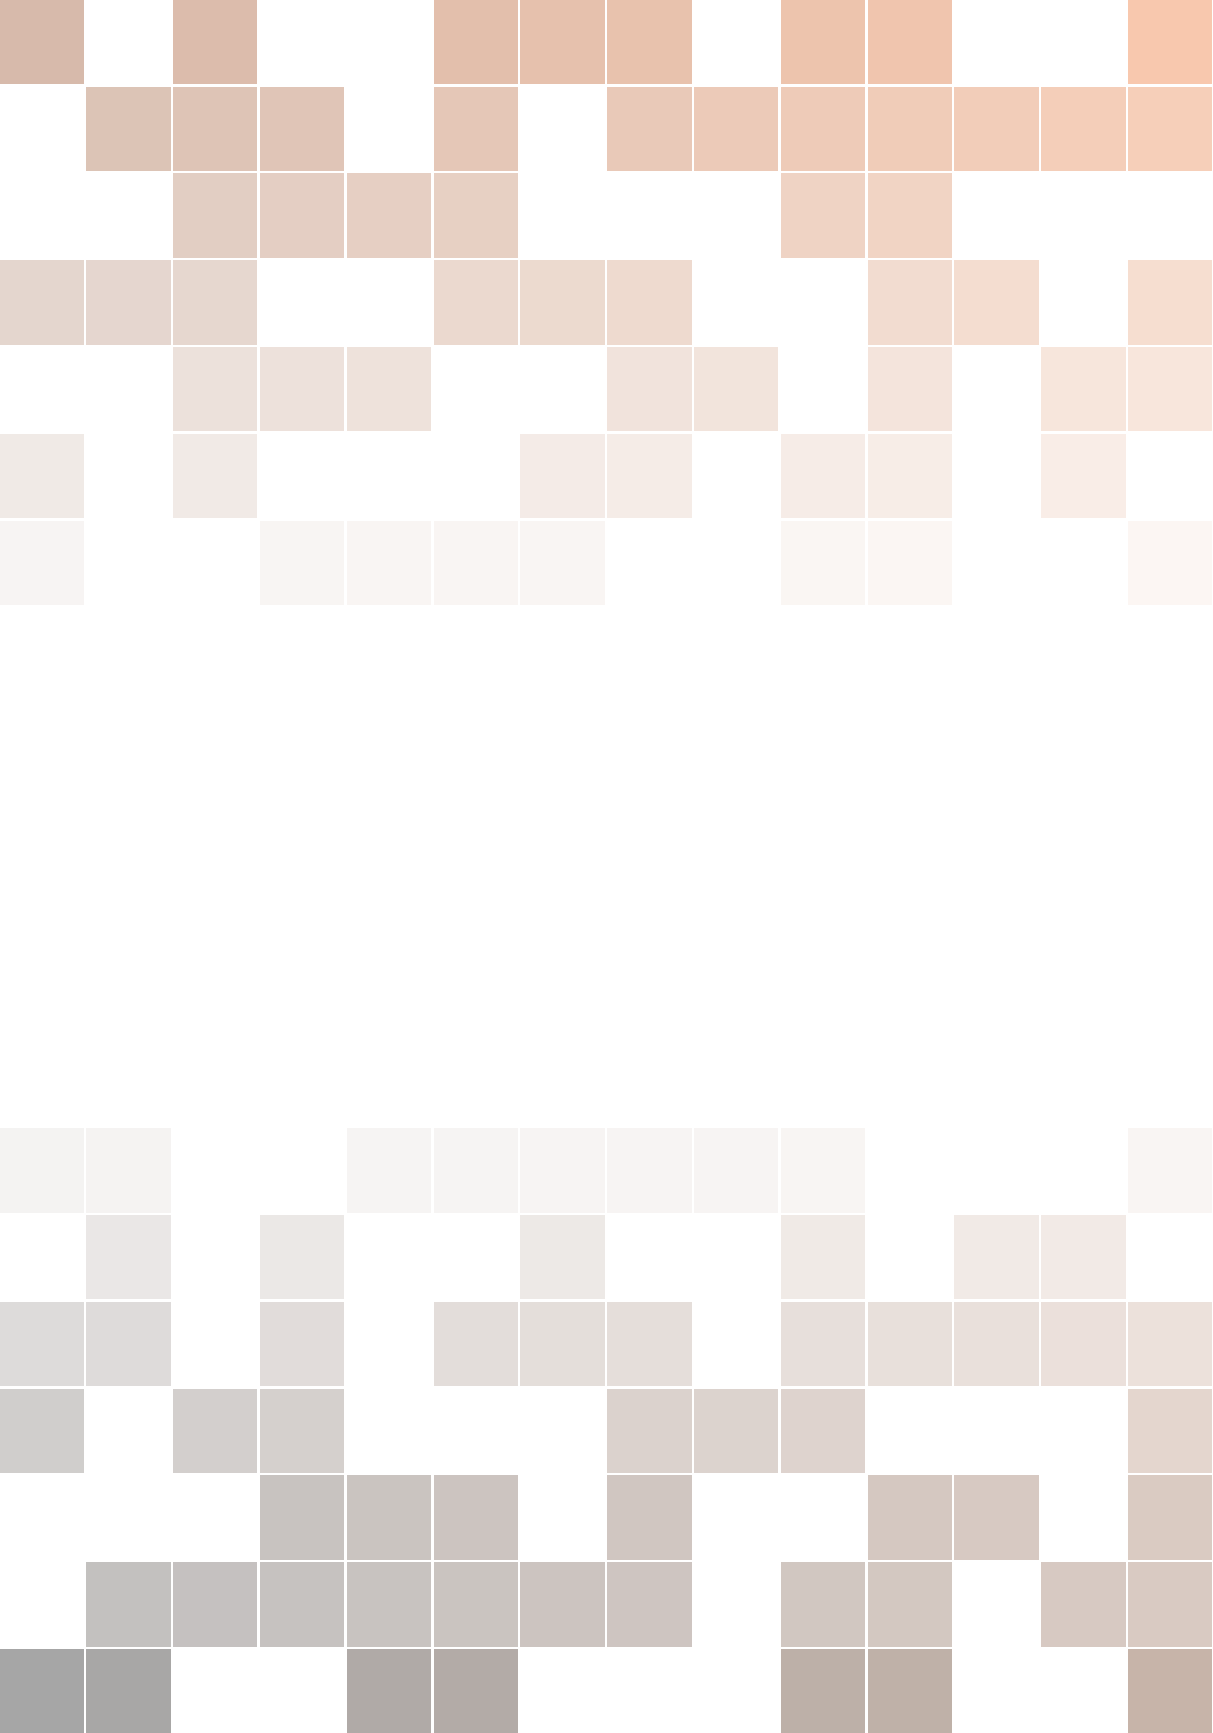
\includegraphics[scale=1]{pics/background}}} % Image background
\centering
\vspace*{9cm}
\par\normalfont\fontsize{35}{35}\sffamily\selectfont
The \muelu tutorial \par % Book title
\vspace*{1cm}
{\Huge \parbox{10cm}{Tobias Wiesner\newline Michael Gee \newline Andrey Prokopenko \newline Jonathan Hu}}\par % Author name
\endgroup

%----------------------------------------------------------------------------------------
%	COPYRIGHT PAGE
%----------------------------------------------------------------------------------------

\newpage
~\vfill
\thispagestyle{empty}

\noindent \textbf{Tobias A. Wiesner}  \\
Institute for Computational Mechanics \\
Technische Universit\"at M\"unchen  \\
Boltzmannstr. 15 \\
85747 Garching\\
Germany\\

\noindent \textbf{Michael W. Gee}\\
Mechanics \& High Performance Computing Group \\
Technische Universit\"at M\"unchen  \\
Parkring 35 \\
85748 Garching\\
Germany\\

\noindent \textbf{Andrey Prokopenko} \\
Scalable Algorithms \\
Sandia National Laboratories\\
Mailstop 1318 \\
P.O.~Box 5800 \\
Albuquerque, NM 87185-1318\\

\noindent \textbf{Jonathan J. Hu} \\
Scalable Algorithms \\
Sandia National Laboratories\\
Mailstop 9159 \\
P.O.~Box 0969 \\
Livermore, CA 94551-0969\\

\noindent Sandia National Laboratories is a multi-program laboratory managed
and operated by Sandia Corporation, a wholly owned subsidiary of Lockheed
Martin Corporation, for the U.S. Department of Energy's National Nuclear
Security Administration under contract DE-AC04-94AL85000 

%\noindent Copyright \copyright\ 2013 John Smith\\ % Copyright notice
%
%\noindent \textsc{Published by Publisher}\\ % Publisher
%

%


%\noindent Licensed under the Creative Commons Attribution-NonCommercial 3.0 Unported License (the ``License''). You may not use this file except in compliance with the License. You may obtain a copy of the License at \url{http://creativecommons.org/licenses/by-nc/3.0}. Unless required by applicable law or agreed to in writing, software distributed under the License is distributed on an \textsc{``as is'' basis, without warranties or conditions of any kind}, either express or implied. See the License for the specific language governing permissions and limitations under the License.\\ % License information

\noindent \textsc{http://trilinos.org/packages/muelu/}\\ % URL

\noindent \textit{SAND2014-18624 R}

\noindent \textit{First printing, September 2014} % Printing/edition date

\noindent {\tiny{\textit{Version: \input{version.txt}}}}

\chapter*{Preface}

\section*{Idea and concept}
The \muelu tutorial is written as a hands-on tutorial for \muelu, the next generation multigrid framework in \trilinos. It covers the whole spectrum from absolute beginners' topics to expert level. Since the focus of this tutorial is on practical and technical aspects of multigrid methods in general and \muelu in particular, the reader is expected to have a basic understanding of multigrid methods and its general underlying concepts. Please refer to multigrid textbooks (e.g. \cite{briggs}) for the theoretical background.

\subsection*{Content}
The tutorial is split into three parts. The first part contains four tutorials for beginners who are interested in using multigrid methods.
No knowledge about C++ is required if the programs are used that come with the tutorial (in the \trilinos repository). If one uses the virtual box image one can even avoid the \trilinos compilation process.
So, the tutorials in the first part can also be used for teaching purposes. One can easily study the smoothing effect of multigrid smoothers and perform some very basic experiments which helps to gain a better understanding of multigrid methods. In the quick start tutorial all steps are documented step by step such that it should be very easy to follow the tutorial. Different exercises may encourage the reader for performing some more experiments and tests. The following tutorials give an overview of the existing level smoothers and transfer operators that can easily be used with the simple XML format \muelu uses for defining the multigrid hierarchies. In addition, it is explained how to visualize the aggregates and export the multigrid levels for a more in-depth analysis.

The second part consists of five tutorials which are for users which are interested in some more background on the underlying techniques that are used in \muelu. The user still does not need explicit knowledge of C++ or any other programming language, but some interest in object-oriented design concepts may be helpful to understand the factory concept. The focus of the second part is on the introduction of the advanced XML interface for \muelu which describes all internal building blocks of the multigrid setup procedures with its internal dependencies. In context of transfer operator smoothing a brief introduction of the theory is given with some in-depth details on the algorithmic design in \muelu. More advanced topics such as rebalancing are handled as well as aggregation strategies. Additional exercises help the reader to perform some experiments in practice.

The third part is meant for expert users who want to use \muelu within their own software. Many detailed C++ examples show how to use \muelu from an user application as preconditioner for a Krylov subspace method or as a standalone multigrid solver. We expect the reader to be familiar with \trilinos, especially with the linear algebra packages \epetra and \tpetra as well as the linear solver packages \aztecoo or \belos. For users who are already using \ml, the predecessor multigrid package of \muelu in \trilinos, we provide a chapter describing the migration process from \ml to \muelu.

\section*{References}

For a complete overview of all features and available parameters in \muelu the reader may refer to the \muelu user guide \cite{Mue}. For the most current version of \muelu it is recommended to visit the homepage 
\begin{verbatim}
http://trilinos.org/packages/muelu/
\end{verbatim}
If you find errors in this tutorial, please contact the \muelu user list 
\begin{verbatim}
muelu-users@software.sandia.gov
\end{verbatim}

\section*{Acknowledgments}
Many people have helped to develop \muelu, and we would like to acknowledge their contributions: Tom Benson, Julian Cortial, Jeremie Gaidamour, Axel Gerstenberger, Chetan Jhurani, Mark Hoemmen, Jonathan Hu, Paul Lin, Eric Phipps, Andrey Prokopenko, Chris Siefert, Paul Tsuji, Ray Tuminaro, and Tobias Wiesner.

\part{Beginners tutorial}

\lstset{
  breaklines=true,                % sets automatic line breaking
}



%\chapterimage{chapter_head_1.pdf} % Table of contents heading image
\chapterimage{pics/ch_bg1_small.png} % Table of contents heading image
\chapter{Quick start}

The first example is meant to quickly get into touch with \muelu. 

\section{Example problem}
\label{lab:examplesym}
We generate a test matrix corresponding to the stencil of a 2D Laplacian operator on a structured Cartesian grid. The matrix stencil is
\begin{equation}
\label{lab:eq1}
\frac{1}{h^2}\begin{pmatrix} & -1 & \\ -1 & 4 & -1 \\ & -1 & \end{pmatrix}.
\end{equation}
The resulting matrix is symmetric positive definite. We choose the right hand side to be the constant vector one and use a random initial guess for the iterative solution process. The problem domain is the unit cube with a Cartesian (uniform) mesh.

\section{User interface}
For this tutorial there is an easy-to-use user interface to perform some experiments with multigrid methods for the given problem as described in \S\ref{lab:examplesym}.
To use the user-interface run
\begin{verbatim}
./hands-on.py
\end{verbatim}
in a terminal in the \texttt{doc/Tutorial/src} folder.

First one has to choose a problem. For this tutorial the right choice is the option 0 for the Laplace 2D problem on a $50\times 50$ mesh.
\begin{center}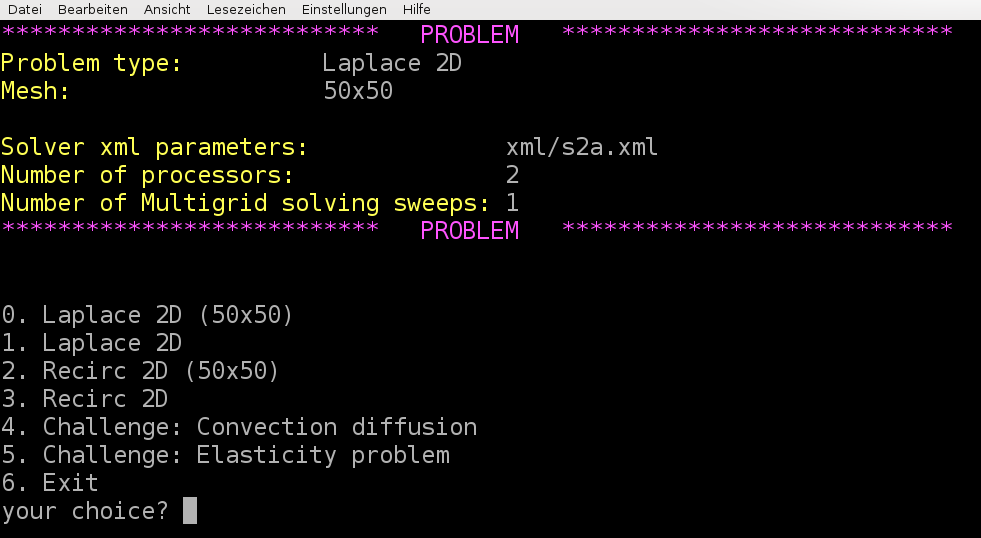
\includegraphics[width=10cm]{pics/tut1_1.png} \end{center}

Next one has to choose a xml file with the multigrid parameters. Choose option 2 and put in \texttt{xml/s1\_easy.xml} as filename for the xml file containing the xml parameters that are used for the multigrid method.
\begin{mycomment}
Please make sure that you enter a filename that actually exists on your hard disk!
\end{mycomment}

\begin{center}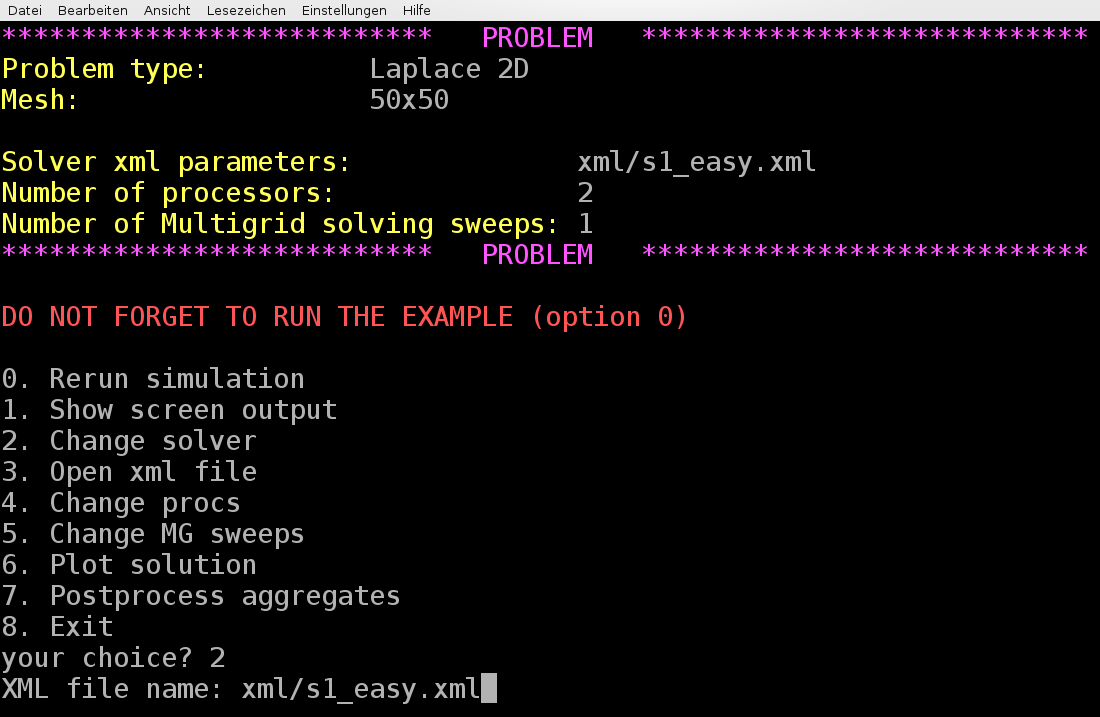
\includegraphics[width=10cm]{pics/tut1_3.png} \end{center}

The \texttt{s1\_easy.xml} file has the following content
\small
\lstinputlisting{../src/xml/s1_easy.xml}
\normalsize
As one can easily find from the xml parameters, a multigrid method with not more than 3 levels and a damped Jacobi method for level smoothing shall be used.

Next, choose option 0 and run the example. That is, the linear system is created and iteratively solved both by a preconditioned CG method (from the \aztecoo package) with a \muelu multigrid preconditioner and a standalone multigrid solver (again using \muelu) with the given multigrid parameters.
\begin{center}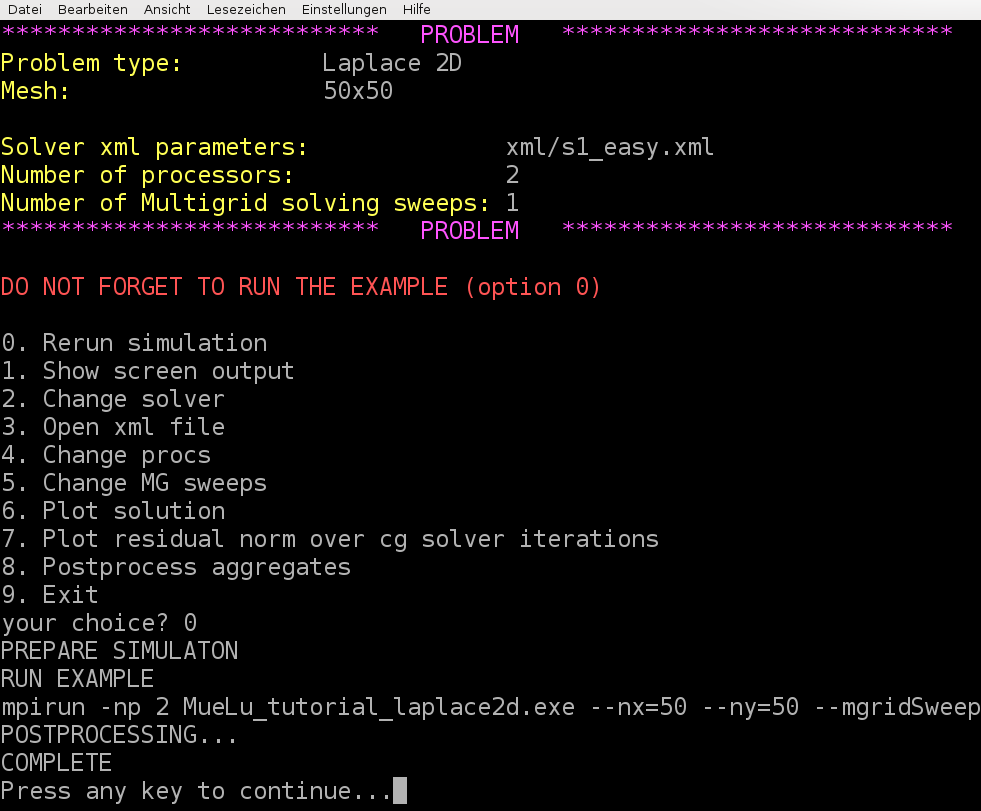
\includegraphics[width=10cm]{pics/tut1_4.png} \end{center}
Note that the line \texttt{mpirun -np 2 MueLu\_tutorial\_laplace2d.exe --nx ...} is the command that is executed in the background. Per default are 2 processors used.

After pressing a key we are ready for a first analysis as it is stated by the green letters \textit{Results up to date!}
\begin{center}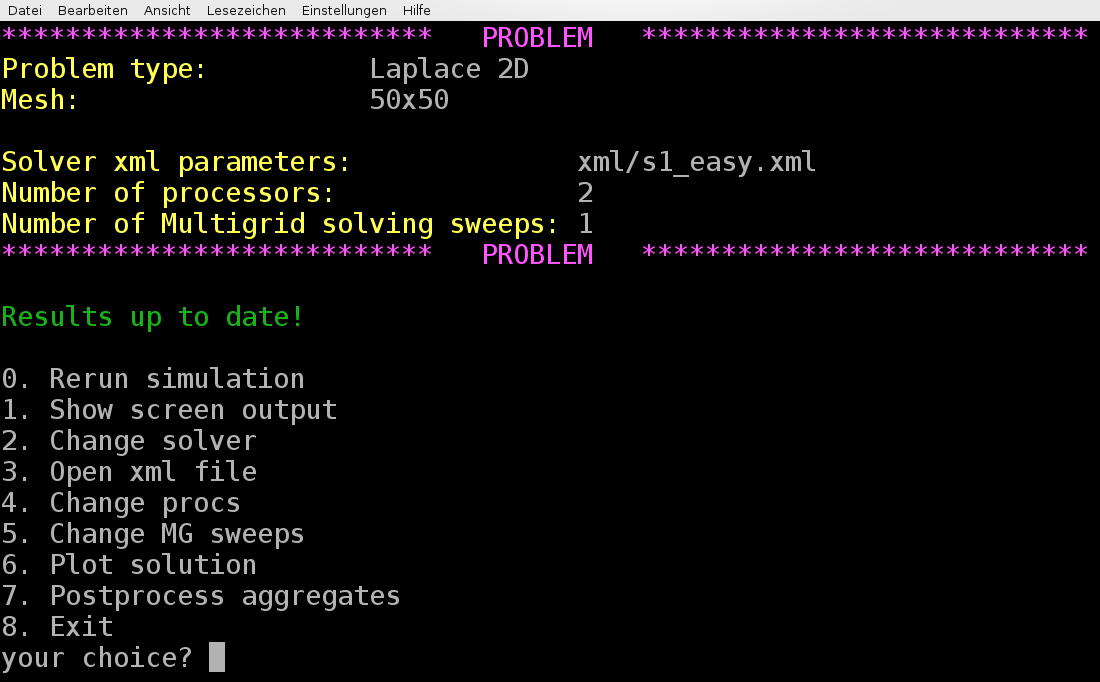
\includegraphics[width=10cm]{pics/tut1_5.png} \end{center}
\begin{mycomment}
If the results are not up to date always choose option 0 first to recalculate the results.
\end{mycomment}

To check the output select option 1 and you should find the following screen output
This should produce the following output on screen.

\printScreenOutput{s1_easy.txt_3.fragment_1.fragment}

\begin{mycomment}
Depending on the number of lines in your terminal you may have to scroll up to the top of the file.
\end{mycomment}

These lines give you some information about the setup process with some details on the aggregation process and the transfer operators. Note that for this example three levels are built (Level 0 for the finest level, level 1 as inter-medium level and level 2 for the coarsest level). Then an overview of the different multigrid levels is given by

\printScreenOutput{s1_easy.txt_3.fragment_3.fragment}

One can see that a three level multigrid method is used with a direct solver on the coarsest level and Jacobi level smoothers on the fine and inter-medium level. Furthermore some basic information is printed such as the operator complexity.

In the end the CG convergence is printed when applying the generated multigrid method as preconditioner within a CG solver from the \aztecoo package in \trilinos.
The numbers give the relative residual after the corresponding number of iterations as well as the solution time in seconds.
\printScreenOutput{s1_easy.txt_5.fragment}

Selecting option 6 gives you four plots.
\begin{center}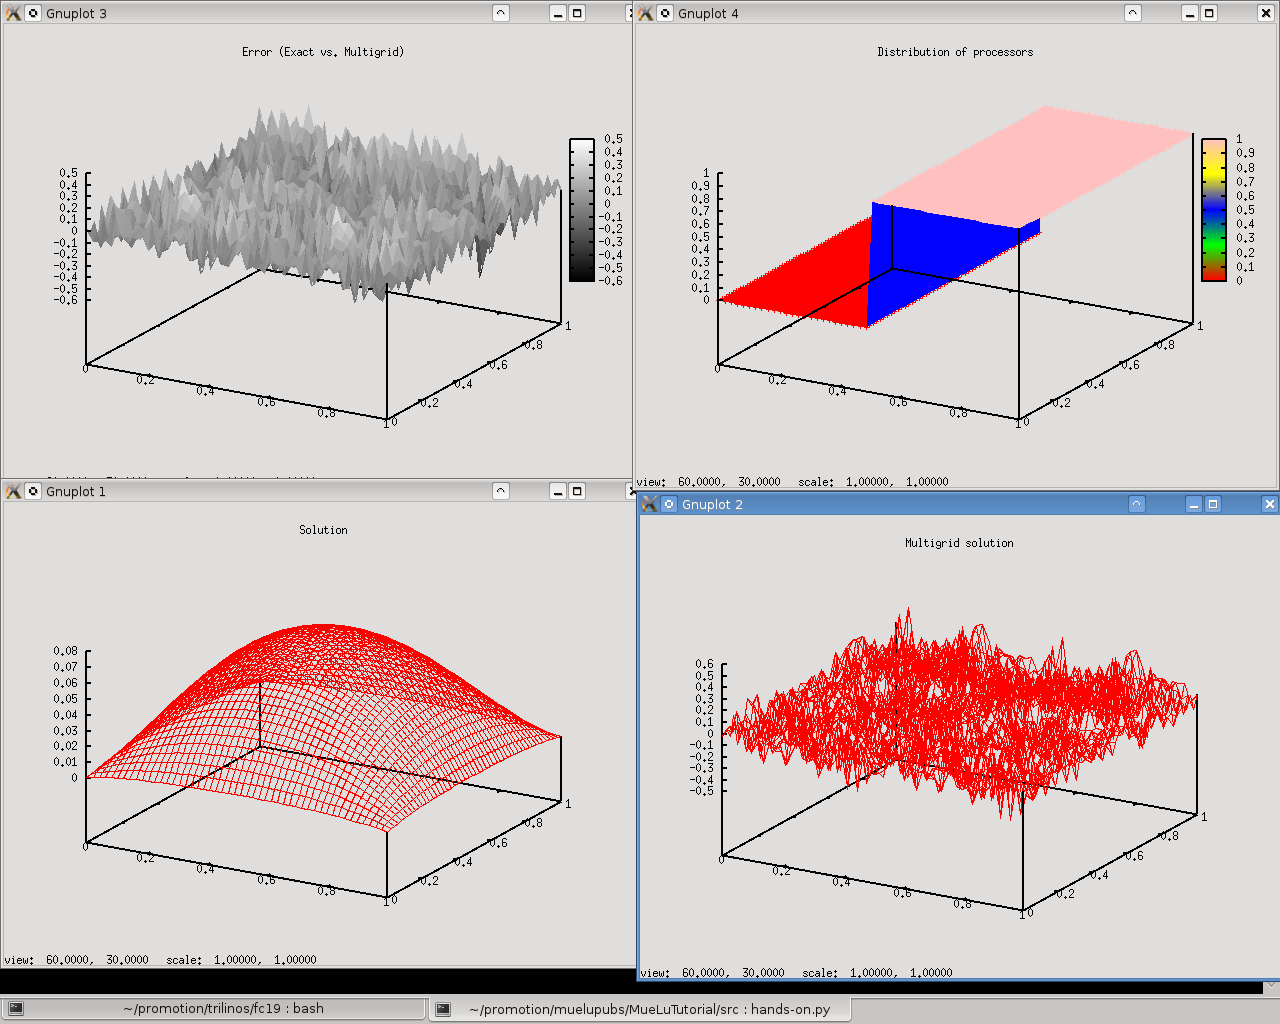
\includegraphics[width=10cm]{pics/tut1_6.png} \end{center}
The lower left plot shows the exact solution of the linear system (using a direct solver from the \amesos package). The lower right plot shows the multigrid solution when 1 sweep with a V-cycle of the multigrid method as defined in the xml parameter file is applied to the linear system as a standalone multigrid solver. As one can see, the multigrid solution with a random initial guess is far away from the exact solution. The upper left plot shows the difference between the multigrid solution and the exact solution. Finally, the upper right plot shows the distribution of the fine level mesh nodes over the processors (in our example we use 2 processors).

\begin{mycomment}
Note, that the plots do not show the solution of the preconditioned CG method! The solution of the CG method is always exact up to a given tolerance as long as the multigrid preconditioner is sufficient. This can be checked by the screen output under option 1.
\end{mycomment}

As a first experiment we change the number of multigrid sweeps for the stand alone multigrid smoother. Let's choose option 5 and use 10 multigrid sweeps.
\begin{center}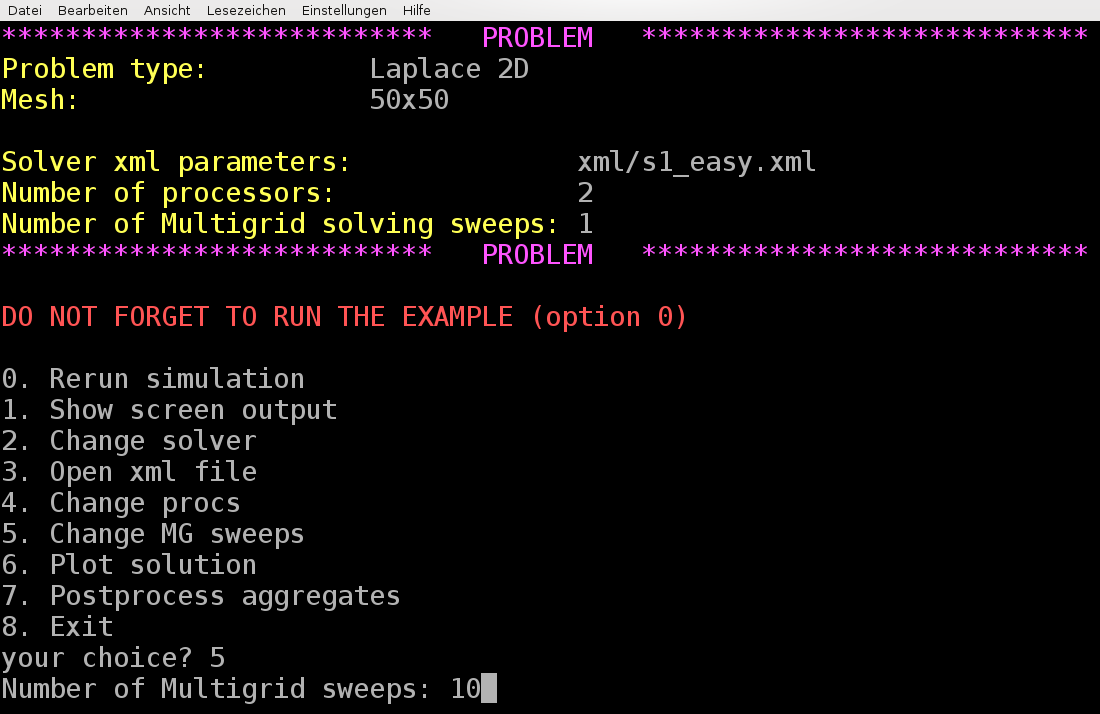
\includegraphics[width=10cm]{pics/tut1_7.png} \end{center}
Then, do not forget to rerun the examples to update the results. That is, choose option 0 and wait for the simulation to finish. Then plot again the results using menu option 6 and you should obtain
\begin{center}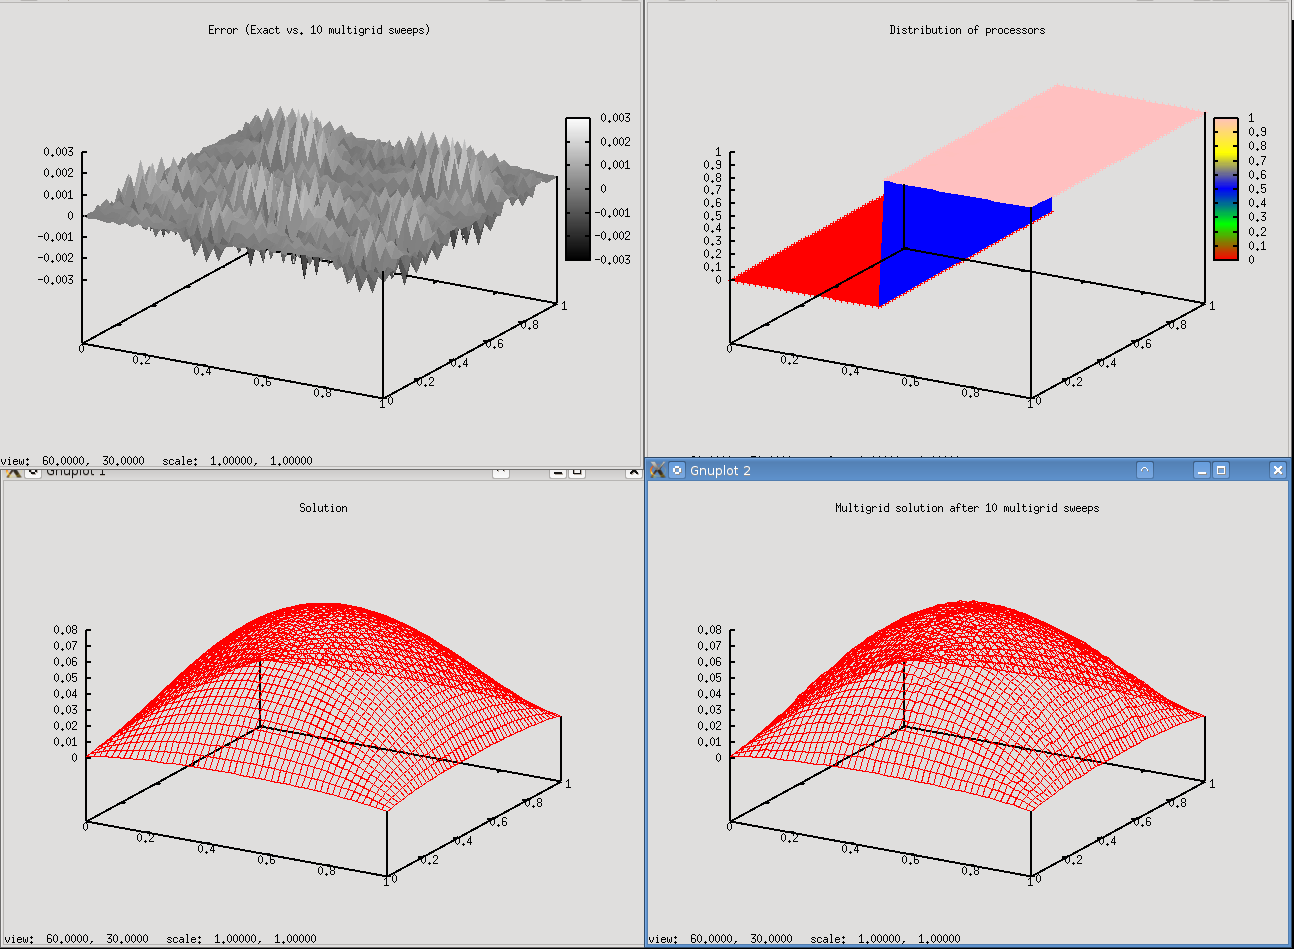
\includegraphics[width=10cm]{pics/tut1_8.png} \end{center}
As one can see is the multigrid solution rather close to the exact solution. In the error plot one finds some low and high frequency error components.

\begin{exercise}
Change the number of processors. Use option 4 and select for example 4 processors (instead of 2). Rerun the example and plot the results.
\begin{center}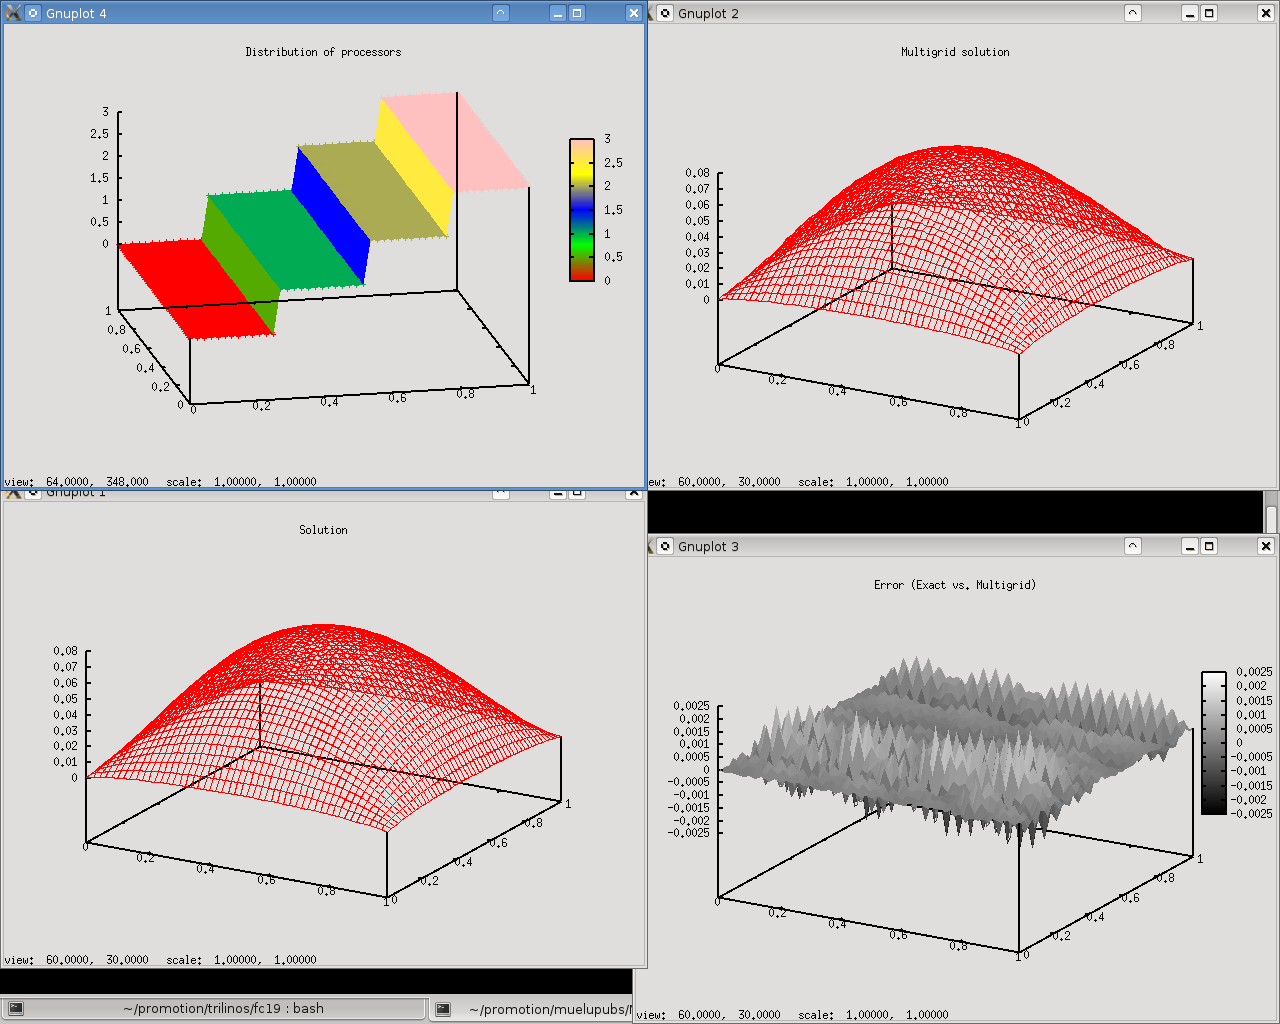
\includegraphics[width=10cm]{pics/tut1_9.png} \end{center}
\end{exercise}
\begin{exercise}
Compare the output when using 4 processors with the output for only 2 processors. Is the number of aggregates changing? Is there some effect on the quality of the multigrid solution. How does the number and convergence history change for the preconditioned CG method?
\end{exercise}
\begin{exercise}
Choose option 8 to close the program.
\end{exercise}

\section{The XML input deck -- multigrid parameters}

After we have learned the basics of the driver program for our experiments we now perform some experiments with our multigrid methods. We again use the simple 2D Laplace problem. First, we create a copy of the solver parameters using 
\begin{verbatim}
cp xml/s1_easy.xml mysolver.xml
\end{verbatim}
Then, we run the driver program again using 
\begin{verbatim}
./hands-on.sh
\end{verbatim}
and choose option 0 for the 2D Laplace example on the $50\times 50$ mesh. Use the xml parameters from the \texttt{mysolver.xml} file, that is, choose option 2 and put in \texttt{mysolver.xml}. Make sure that the problem can be solved with the parameters (option 0) and verify the solver output.

Once that is done it is time for some first experiments. Open you \texttt{mysolver.xml} file in a text editor. You can try option 3 for doing that, but alternatively you can also do it by hand choosing your favorite text editor.

\begin{center}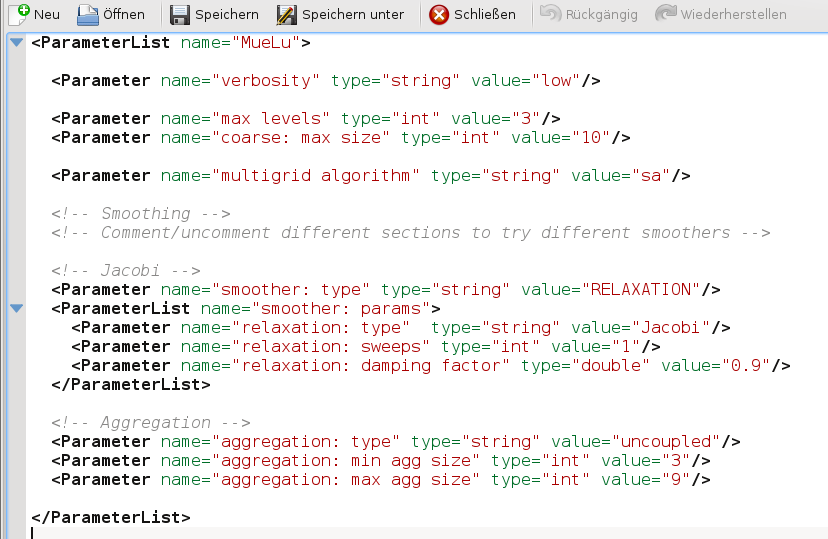
\includegraphics[width=\textwidth]{pics/tut1_10.png} \end{center}

Now, let's change the maximum number of multigrid levels from 3 to 10 in the xml file, that is, change the value of the parameter \textit{max levels} from 3 to 10. Do not forget to save the file and rerun the example by choosing option 0 in the driver program.
The screen output should be the following

\printScreenOutput{s1_easy_10levels.txt_3.fragment_3.fragment}

Note that even though we allow for at maximum 10 multigrid levels the coarsening process stops after level 4. The reason is that the linear operator on multigrid level 4 has only 4 lines and therefore is smaller than the \texttt{coarse: max size} parameter in the xml parameter list which defines the maximum size of the linear operator on the coarsest level.


\begin{exercise}
How do you have to choose the \texttt{coarse: max size} parameter to obtain a 3 level multigrid method again? Increase the parameter accordingly, rerun the simulation and check your results.
\end{exercise}
\begin{exercise}
What happens if you allow only for a 1 level method (i.e., no multigrid)? How does this affect the preconditioned CG method?
\end{exercise}

The option \texttt{sa} for \textit{smoothed aggregation} in the \texttt{multigrid algorithm} parameter can be considered to be optimal for symmetric positive definite problems. We can compare it with the option \texttt{unsmoothed} as a robust but slower alternative. Let's choose a 3 level multigrid method with unsmoothed transfer operators (i.e., \texttt{max levels = 3}, \texttt{multigrid algorithm = unsmoothed}), then we obtain
\printScreenOutput{s1_easy_3levels_unsmoothed.txt_5.fragment}

Compared with the smoothed aggregation method (\texttt{multigrid algorithm = sa}) which uses some smoothed transfer operator basis functions within the multigrid method, the unsmoothed multigrid algorithm needs a significantly higher number of iterations.
The same method with smoothed transfer operator basis functions gives
\printScreenOutput{s1_easy_3levels_smoothed.txt_5.fragment}
\begin{mycomment}
You can find the corresponding xml files also in \texttt{xml/s1\_easy\_3levels\_unsmoothed.xml} and \texttt{xml/s1\_easy\_3levels\_smoothed.xml}.
\end{mycomment}

\begin{exercise}
Compare the screen output of the unsmoothed multigrid method and the smoothed aggregation multigrid method. Which parts are missing in the multigrid setup for the unsmoothed multigrid method? How does the multigrid method affect the aggregates?
\end{exercise}
\begin{exercise}
Performing 10 multigrid sweeps both with the unsmoothed and the smoothed aggregation multigrid method gives the following error plots
 \begin{center}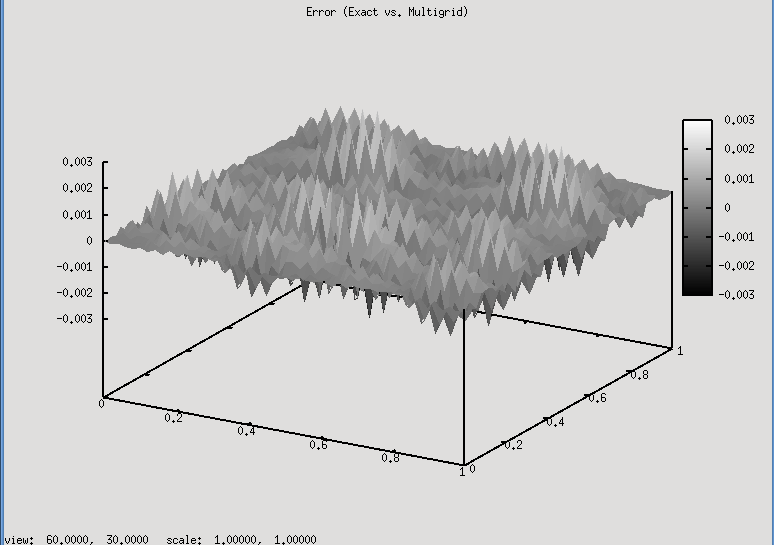
\includegraphics[width=8cm]{pics/tut1_11.png} 
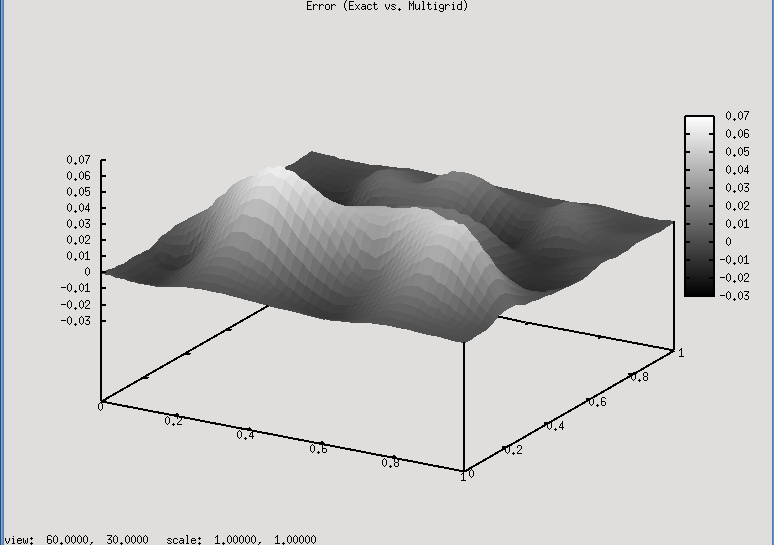
\includegraphics[width=8cm]{pics/tut1_12.png} \end{center}
 Which one belongs to the unsmoothed multigrid method?
\end{exercise}

\chapter{Level smoothers}

From the last tutorial we have learned that the used multigrid algorithm may have a significant influence in the convergence speed. When comparing the error plots for the standalone multigrid smoothers with unsmoothed and smoothed aggregation multigrid one finds also a notable difference in the ``smoothness'' of the error.

\section{Background on multigrid methods}
Obviously there are cases where some highly oscillatory error modes are left and overlaying some low frequency modes. In other cases there are only low frequency error modes left. Theses are basically the two typical cases one might find in practice.

Multigrid methods are based on the fact, that (cheap) level smoothing method often are able to smooth out high oscillatory error components whereas they cannot reduce low frequency error components very well. These low frequency error components then are transferred to a coarse level where they can be seen as high frequency error component for a level smoother on the coarse level.

One should not forget that for an efficient multigrid method both the so-called coarse level correction method and the level smoothers have to work together. That is, one has to choose the right multigrid method (e.g., \texttt{unsmoothed} or \texttt{sa}) in combination with an appropriate level smoothing strategy.

\section{Example}
In context of multigrid level smoothers we have to define both the level smoothers and the coarse solver. Usually, a direct solver is used as coarse solver that is applied to the coarsest multigrid levels. However, it is also possible to apply any other kind of iterative smoothing method or even no solver at all (even though this would be non-standard). The following XML file shows how to use a Jacobi smoother both for level smoothing and as coarse solver.
\lstinputlisting{../src/xml/s1_easy_jacobi.xml}
The corresponding multigrid hierarchy is
\printScreenOutput{s1_easy_jacobi.txt_3.fragment_3.fragment}

Figures \ref{fig:1vcycles} and \ref{fig:5vcycles} show the multigrid effect of different number of Jacobi smoothers on all multigrid levels.

One has even more fine-grained control over pre- and post-smoothing.
\lstinputlisting{../src/xml/s1_easy_jacobi2.xml}
This produces the following multigrid hierarchy
\printScreenOutput{s1_easy_jacobi2.txt_3.fragment_3.fragment}

\begin{mycomment}
Note that the relaxation based methods provided by the \ifpack package are embedded in an outer additive Schwarz method.
\end{mycomment}

Of course, there exist other smoother methods such as polynomial smoothers (Chebyshev) and ILU based methods.
A detailed overview of the different available smoothers can be found in the \muelu users guide. 


\begin{figure}
\subfigure[1 level with 1 Jacobi sweep ($\omega=0.9$)\label{fig:2dlap111}]{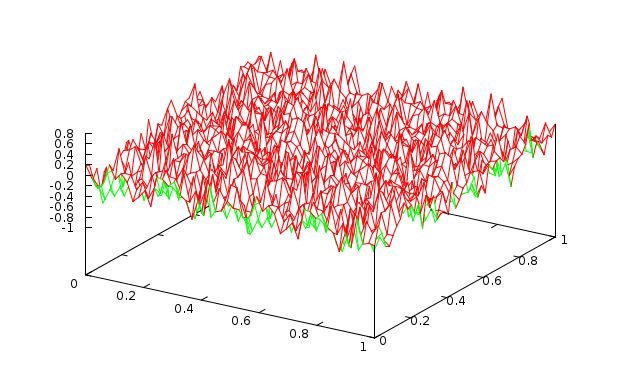
\includegraphics[width=0.3\textwidth]{pics/1level_1jac09.png}}\hspace{0.03\textwidth}
\subfigure[1 level with 10 Jacobi sweeps ($\omega=0.9$)\label{fig:2dlap1110}]{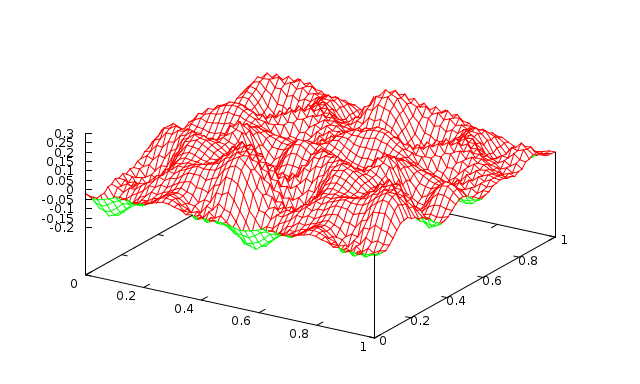
\includegraphics[width=0.3\textwidth]{pics/1level_10jac09.png}}\hspace{0.03\textwidth}
\subfigure[1 level with 100 Jacobi sweeps ($\omega=0.9$)\label{fig:2dlap11100}]{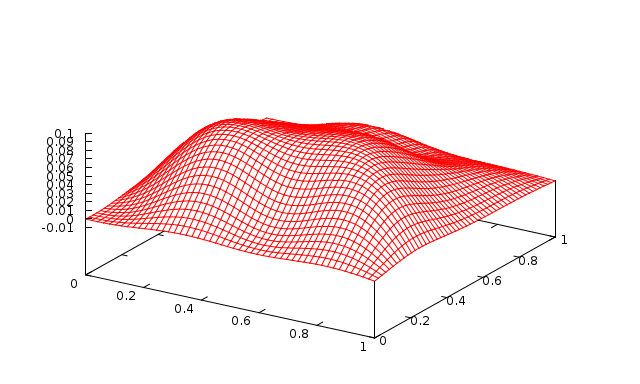
\includegraphics[width=0.3\textwidth]{pics/1level_100jac09.png}} \\
\subfigure[2 level with 1 Jacobi sweep ($\omega=0.9$)\label{fig:2dlap121}]{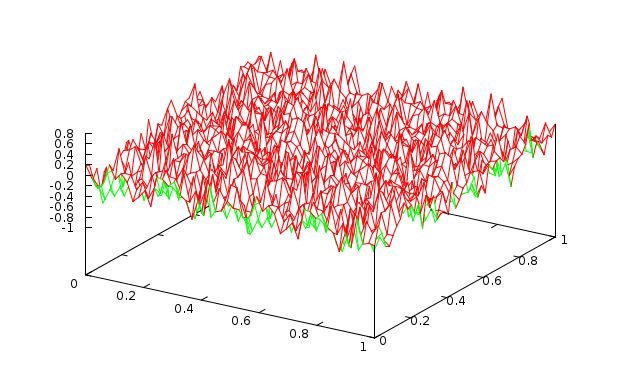
\includegraphics[width=0.3\textwidth]{pics/2level_1jac09.png}}\hspace{0.03\textwidth}
\subfigure[2 level with 10 Jacobi sweeps ($\omega=0.9$)\label{fig:2dlap1210}]{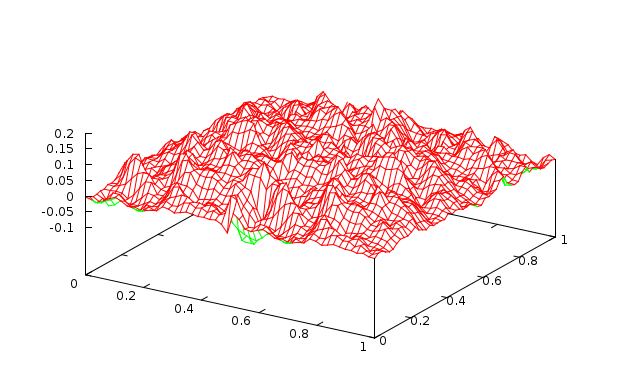
\includegraphics[width=0.3\textwidth]{pics/2level_10jac09.png}}\hspace{0.03\textwidth}
\subfigure[2 level with 100 Jacobi sweeps ($\omega=0.9$)\label{fig:2dlap12100}]{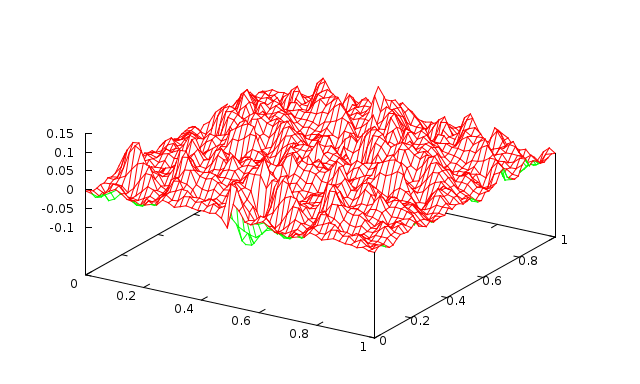
\includegraphics[width=0.3\textwidth]{pics/2level_100jac09.png}} \\
\subfigure[3 level with 1 Jacobi sweep ($\omega=0.9$)\label{fig:2dlap131}]{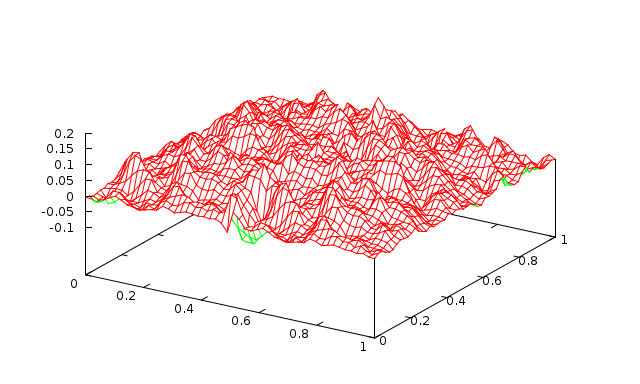
\includegraphics[width=0.3\textwidth]{pics/3level_1jac09.png}}\hspace{0.03\textwidth}
\subfigure[3 level with 10 Jacobi sweeps ($\omega=0.9$)\label{fig:2dlap1310}]{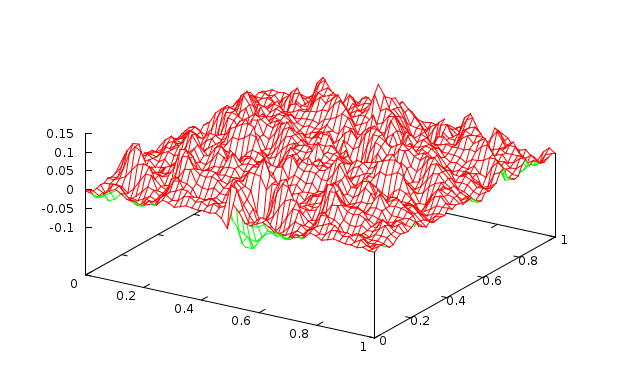
\includegraphics[width=0.3\textwidth]{pics/3level_10jac09.png}}\hspace{0.03\textwidth}
\subfigure[3 level with 100 Jacobi sweeps ($\omega=0.9$)\label{fig:2dlap13100}]{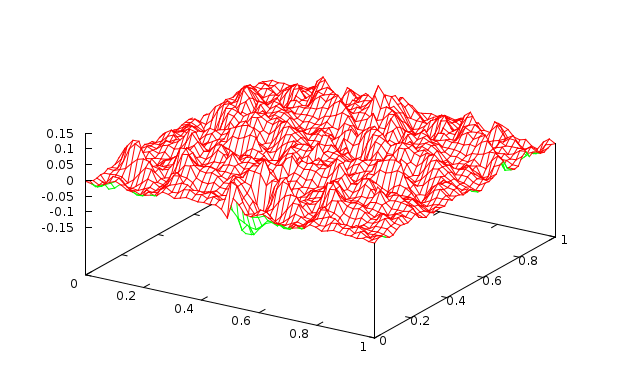
\includegraphics[width=0.3\textwidth]{pics/3level_100jac09.png}} \\
\caption{2D Laplace equation on $50\times 50$ mesh after 1 V-cycle with an AMG multigrid solver and Jacobi smoothers on all multigrid levels. (2 processors)}
\label{fig:1vcycles}
\end{figure}


\begin{figure}
\subfigure[1 level with 1 Jacobi sweep ($\omega=0.9$)\label{fig:2dlap511}]{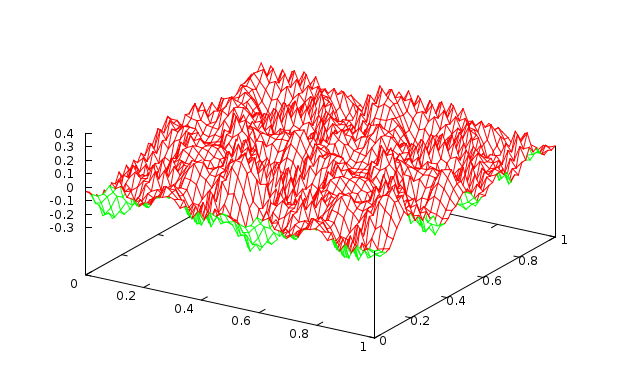
\includegraphics[width=0.3\textwidth]{pics/5sweeps_1level_1jac09.png}}\hspace{0.03\textwidth}
\subfigure[1 level with 10 Jacobi sweeps ($\omega=0.9$)\label{fig:2dlap5110}]{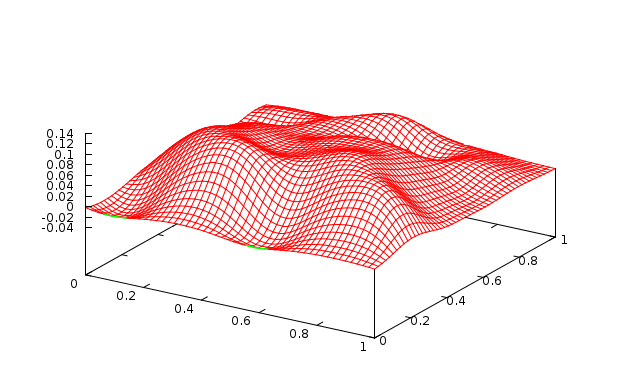
\includegraphics[width=0.3\textwidth]{pics/5sweeps_1level_10jac09.png}}\hspace{0.03\textwidth}
\subfigure[1 level with 100 Jacobi sweeps ($\omega=0.9$)\label{fig:2dlap51100}]{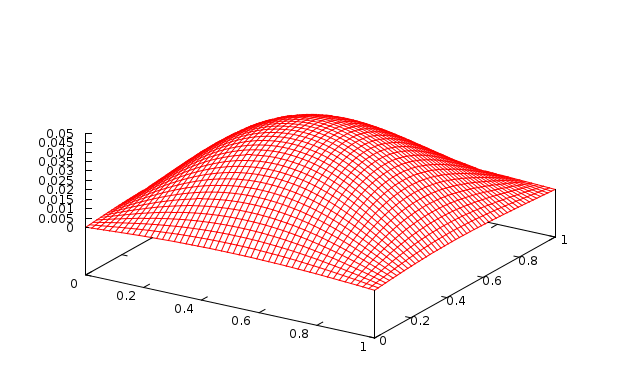
\includegraphics[width=0.3\textwidth]{pics/5sweeps_1level_100jac09.png}} \\
\subfigure[2 level with 1 Jacobi sweep ($\omega=0.9$)\label{fig:2dlap521}]{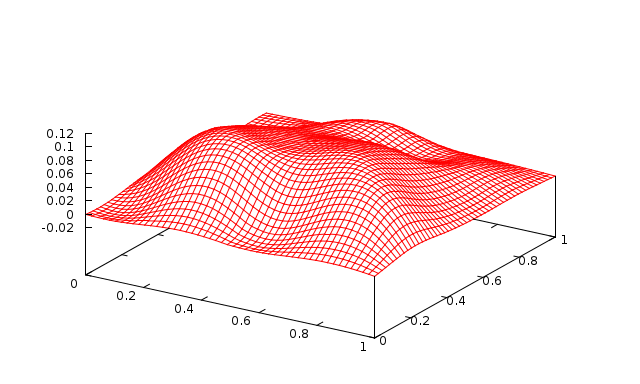
\includegraphics[width=0.3\textwidth]{pics/5sweeps_2level_1jac09.png}}\hspace{0.03\textwidth}
\subfigure[2 level with 10 Jacobi sweeps ($\omega=0.9$)\label{fig:2dlap5210}]{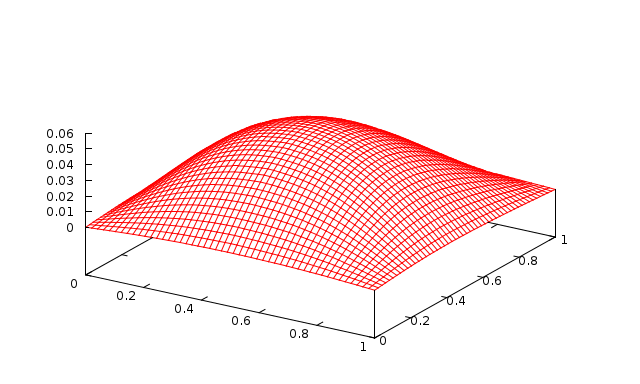
\includegraphics[width=0.3\textwidth]{pics/5sweeps_2level_10jac09.png}}\hspace{0.03\textwidth}
\subfigure[2 level with 100 Jacobi sweeps ($\omega=0.9$)\label{fig:2dlap52100}]{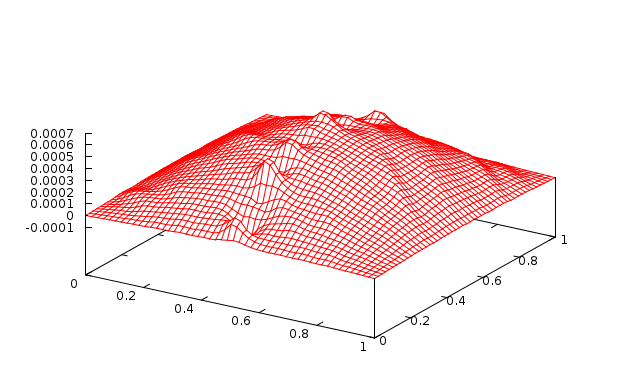
\includegraphics[width=0.3\textwidth]{pics/5sweeps_2level_100jac09.png}} \\
\subfigure[3 level with 1 Jacobi sweep ($\omega=0.9$)\label{fig:2dlap531}]{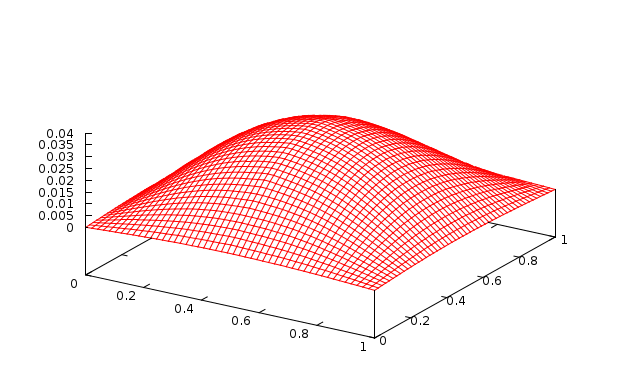
\includegraphics[width=0.3\textwidth]{pics/5sweeps_3level_1jac09.png}}\hspace{0.03\textwidth}
\subfigure[3 level with 10 Jacobi sweeps ($\omega=0.9$)\label{fig:2dlap5310}]{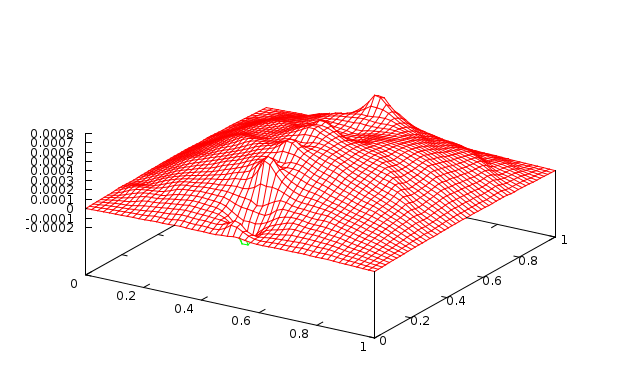
\includegraphics[width=0.3\textwidth]{pics/5sweeps_3level_10jac09.png}}\hspace{0.03\textwidth}
\subfigure[3 level with 100 Jacobi sweeps ($\omega=0.9$)\label{fig:2dlap53100}]{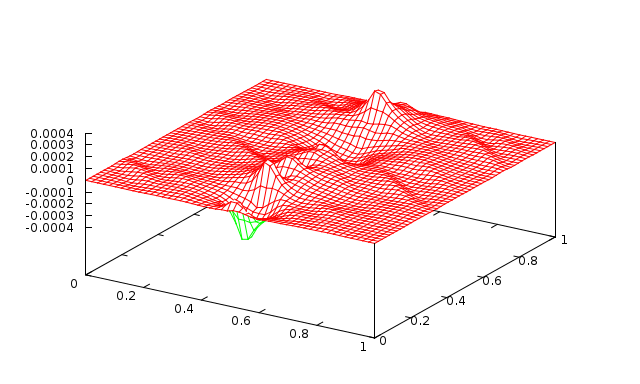
\includegraphics[width=0.3\textwidth]{pics/5sweeps_3level_100jac09.png}} \\
\caption{2D Laplace equation on $50\times 50$ mesh after 5 V-cycle with an AMG multigrid solver and Jacobi smoothers on all multigrid levels. (2 processors)}
\label{fig:5vcycles}
\end{figure}

\begin{exercise}
Play around with the smoother parameters and study their effect on the error plot and the convergence of the preconditioned cg method. For all available smoothing options and parameters refer to the \muelu user guide (\cite{Mue}). Hint: use \texttt{unsmoothed} transfer operator basis functions (i.e., \texttt{multigrid algorithm = unsmoothed}) to highlight the effect of the level smoothers.
\end{exercise}
\begin{exercise}
Use the following parameters to solve the $50\times 50$ Laplace 2D problem on 2 processors
 \lstinputlisting{../src/xml/s1_easy_exercise.xml}
 That is, we change to smoothed aggregation AMG. You can find the xml file also in \texttt{xml/s1\_easy\_exercise.xml}.
 Run the example on 2 processors and check the number of linear iterations and the solver timings in the screen output.
 Can you find smoother parameters which reduce the number of iterations? Can you find smoother parameters which reduce the iteration timings?
\end{exercise}

\chapter{Multigrid for non-symmetric problems}

\section{Test example}
\label{sec:recircexample}
The \texttt{Recirc2D} example uses a matrix corresponding to the finite-difference discretization of the problem
\begin{displaymath}
-\varepsilon\Delta u + (v_x,v_y)\cdot \nabla u=f
\end{displaymath}
on the unit square, with $\varepsilon=1e-5$ and homogeneous Dirichlet boundary conditions. It is $v_x=4x(x-1)(1-2y)$ and $v_y=-4y(y-1)(1-2x)$.
The right hand side vector $f$ is chosen to be the constant vector 1. Due to the convective term the resulting linear system is non-symmetric and therefore more challenging for the iterative solver. The multigrid algorithm has to be adapted to the non-symmetry to obtain good convergence behavior.

\section{User interface}

For this tutorial again we can use the easy-to-use user interface. Run the \texttt{hands-on.py} script in your terminal and choose option 2 for the \texttt{Recirc 2D} example on a $50\times 50$ mesh.
Choose the parameters from the \texttt{n1\_easy.xml} file. If you run the example you might find that the CG method did not converge within 50 iterations.
\begin{center}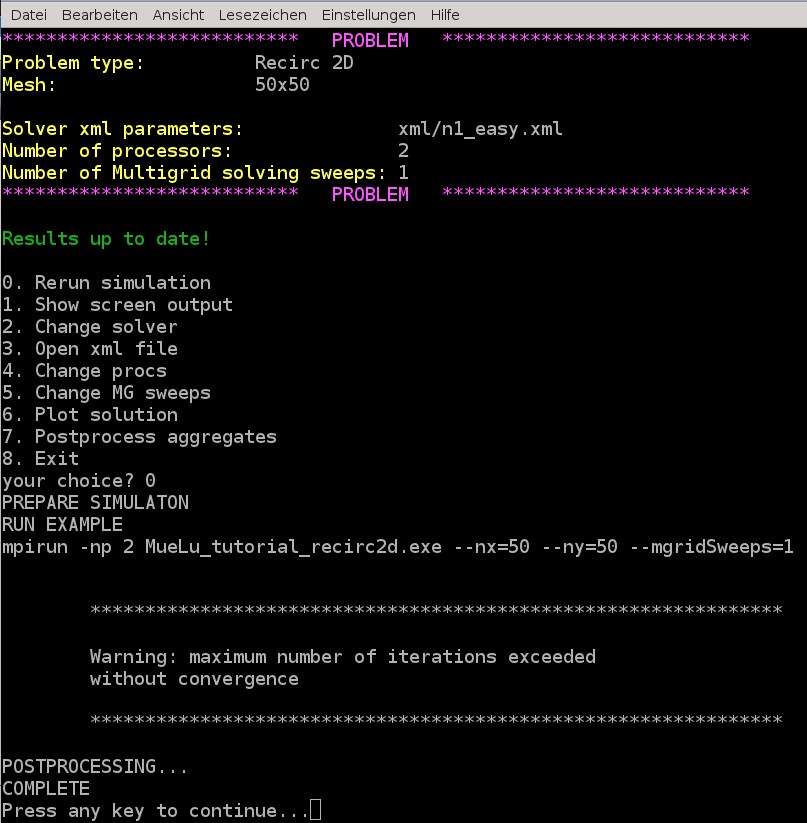
\includegraphics[width=10cm]{pics/tut1_13.png} \end{center}

The convergence of the used unsmoothed transfer operators (\texttt{multigrid algorithm = unsmoothed}) is not optimal. In case of symmetric problems one can reduce the number of iterations using smoothed aggregation algebraic multigrid methods. In context of non-symmetric problems, especially when arising from problems with (highly) convective phenomena, one should use a Petrov-Galerkin approach for smoothing the prolongation and restriction operators more carefully.


\begin{exercise}
Use \texttt{multigrid algorithm = pg} and compare the results with \texttt{multigrid algorithm = unsmoothed}. What is the difference in the number of CG iterations? What is changing in the multigrid setup?
\end{exercise}
\begin{exercise}
For slightly non-symmetric problems the \texttt{sa} method often performs satisfactorily. Change the verbosity to high (\texttt{verbosity = high}) and compare the results of the \texttt{multigrid algorithm = pg} option with the \texttt{multigrid algorithm = sa} option. Try different values between 0 and 1.5 for the damping parameter within the smoothed aggregation method (i.e., try values 0.0, 0.5, 1.0, 1.33 and 1.5 for \texttt{sa: damping factor}). What do you observe?
\end{exercise}

\chapter{Useful tools for analysis}

\section{Visualization of aggregates}

\subsection{Technical prerequisites}
\muelu allows to export plain aggregation information in simple text files that have to be interpreted by some post-processing scripts to generate pictures from the raw data. The post-processing script provided with the \muelu tutorial is written in python and produces VTK output. Please make sure that you have all necessary python packages installed on your machine (including \verb|python-vtk|).

\begin{mycomment}
The visualization script has successfully been tested with VTK 5.x. Note that it is not compatible to VTK 6.x.
\end{mycomment}

\subsection{Visualization of aggregates with \muelu using VTK}
We can visualize the aggregates using the vtk file format and paraview. First add the parameter \texttt{aggregation: export visualization data = true} to the list of aggregation parameters. Use, e.g., the following xml file
\lstinputlisting{../src/xml/n2_easy_agg.xml}
The file is stored in \texttt{xml/n2\_easy\_agg.xml}.

Run the \texttt{hands-on.py} script and select, e.g., the Laplace 2D example on a $50\times 50$ mesh. Select above xml file for the multigrid parameters with the \texttt{aggregation: export visualization data} enabled. Run the program and then choose option 7 for post-processing the aggregates.
\begin{center}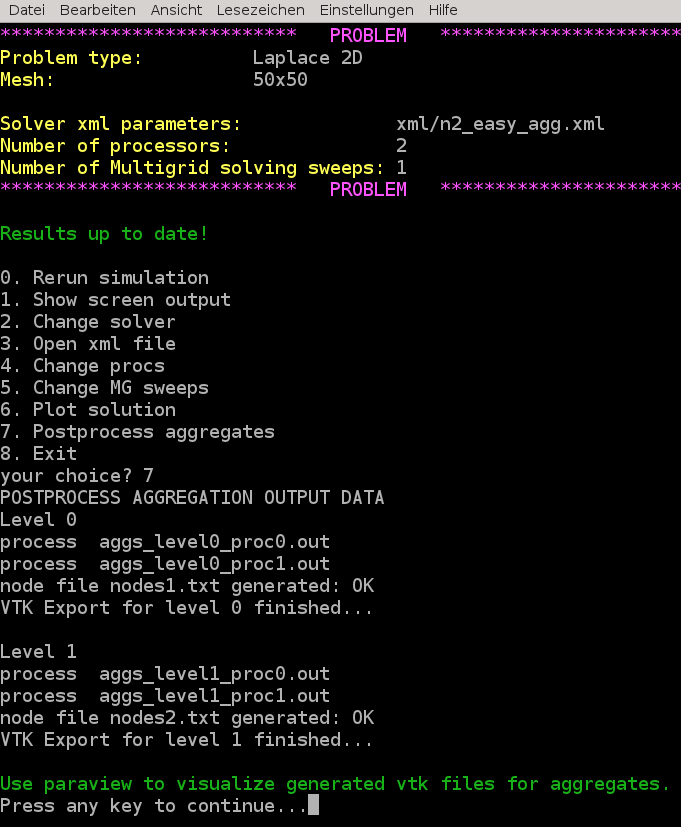
\includegraphics[width=10cm]{pics/tut1_14.png} \end{center}
\begin{mycomment}
Be aware that without \texttt{aggregation: export visualization data = true} the post processing step for the aggregates will fail.
\end{mycomment}

Once the visualization data is exported and post-processed you can run \texttt{paraview} (if it is installed on your machine) and open the files \texttt{aggs0.vtp} and \texttt{aggs1.vtp} for visualization.

Start \verb|paraview| and open the files \texttt{aggs0.vtp} and/or \texttt{aggs1.vtp}. Do not forget to press the \verb|Apply| button to show the aggregates on screen.
\begin{center}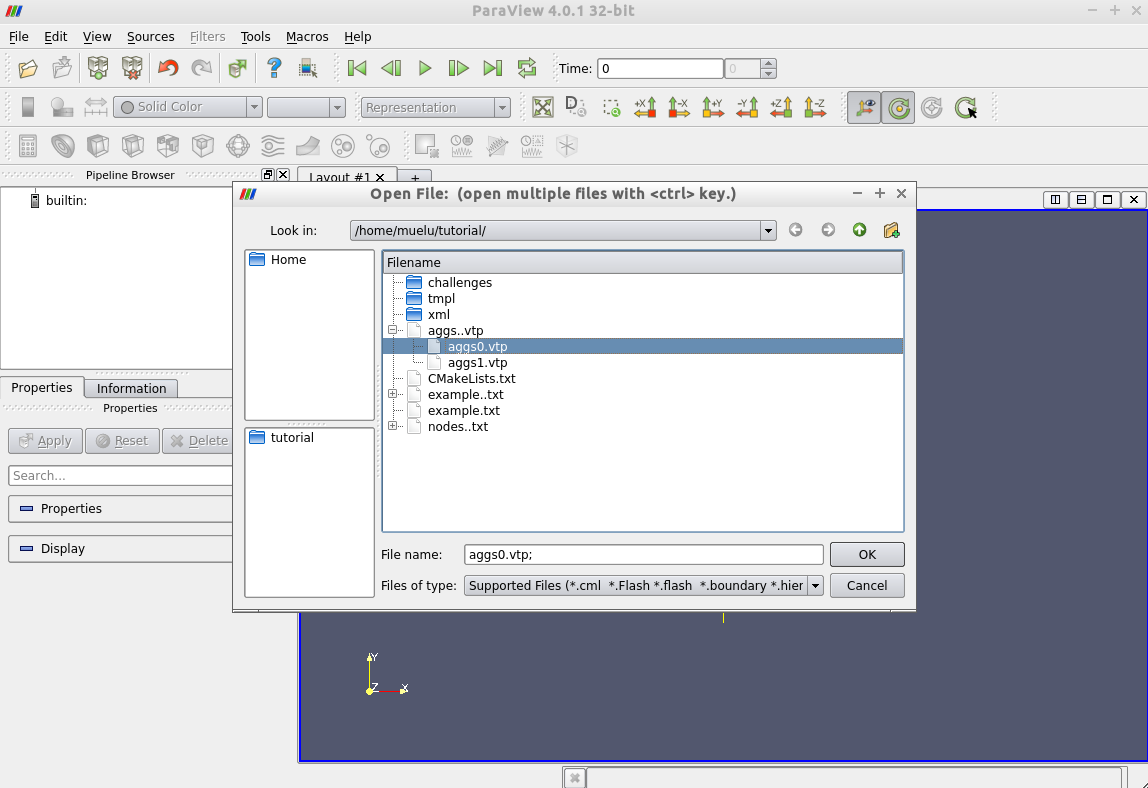
\includegraphics[width=\textwidth]{pics/tut1_17.png} \end{center}
Then the aggregates should be visualized as follows.
\begin{center}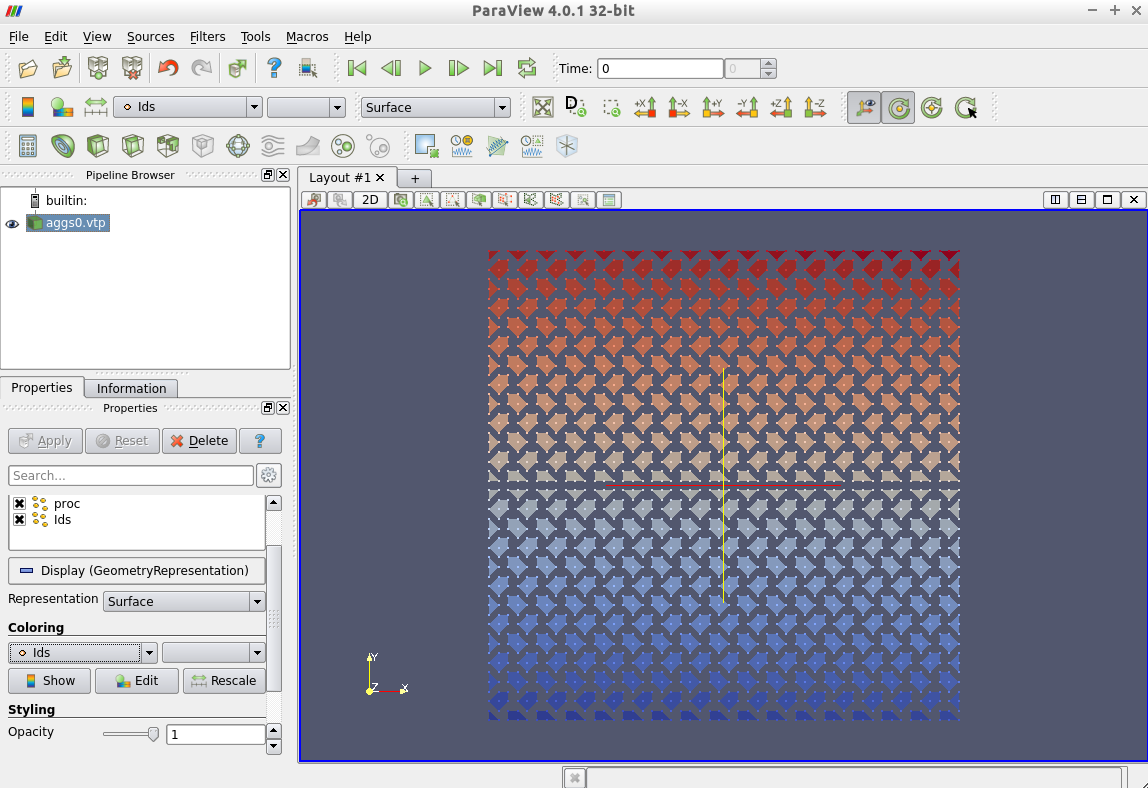
\includegraphics[width=\textwidth]{pics/tut1_18.png} \end{center}
Here the colors represent the unique aggregate id. You can change the coloring in the left column from \verb|Ids| to \verb|proc| which denotes the owning processor of the aggregate.

Figure \ref{fig:symAggs} shows the aggregates for the Laplace2D problem on the different multigrid levels starting with an isotropic $50\times 50$ mesh. No dropping of small entries was used when building the matrix graph (\texttt{aggregation: drop tol=0.0}). For visualization purposes the ``midpoint'' of each aggregate defines the coordinate of the supernode on the next coarser level. Be aware that these supernodes are purely algebraic. There is no coarse mesh for algebraic multigrid methods. As one can see from the colors an uncoupled aggregation strategy has been applied using 2 processors. The aggregates do not cross the processor boundaries.

\begin{figure}
\centering
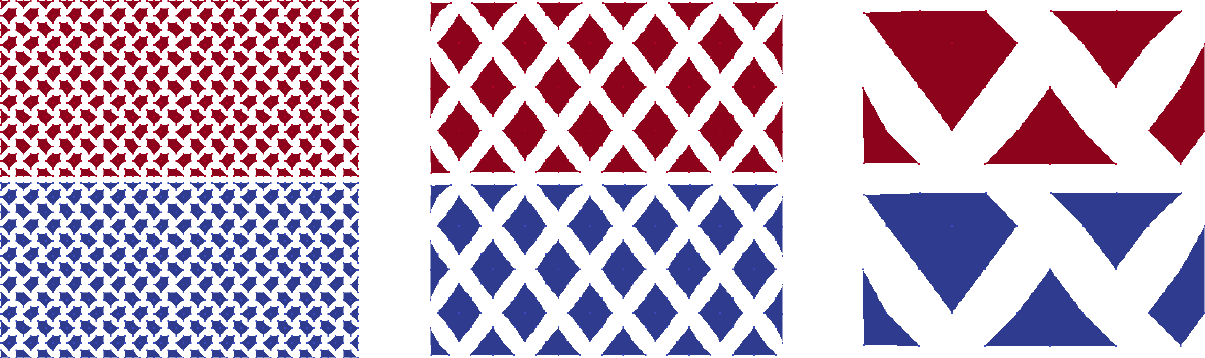
\includegraphics[width=0.7\textwidth]{pics/aggsSymm.png}
\caption{Aggregates for Laplace2D example on $50\times 50$ mesh without dropping.}
\label{fig:symAggs}
\end{figure}

\begin{exercise}
Repeat above steps for the \verb|Recirc2D| example on a $50\times 50$ mesh. Compare the aggregates from the \verb|xml/n2_easy_agg.xml| parameter file with the aggregates when using the \verb|xml/n2_easy_agg2.xml| parameter file, which drops some small entries of the fine level matrix $A$ when building the graph.
\end{exercise}
\begin{exercise}
Vary the number of processors. Do not forget to export the aggregation data (option 7) after the simulation has rerun with a new number of processors. In \verb|paraview| choose the variable \verb|proc| for the coloring. Then the color denotes the processor the aggregate belongs to. How do the aggregates change when switching from 2 to 3 processors?
%  \item Try the solver parameters from \verb|xml/s4c.xml| vor the \verb|Recirc2D| example on a $50\times 50$ mesh and compare them with the results for the \verb|xml/s4a.xml| and \verb|xml/s4b.xml| parameters. Which differences do you observe?
\end{exercise}

Figure \ref{fig:nonsymAggs} shows the aggregates for the Recirc2D problem. When building the matrix graph, entries with values smaller than $0.01$ were dropped. Obviously the shape of the aggregates follows the direction of convection of the example. Using an uncoupled aggregation method (i.e., \texttt{aggregation: type = uncoupled}) as default the aggregates do not cross processor boundaries.
\begin{figure}
\centering
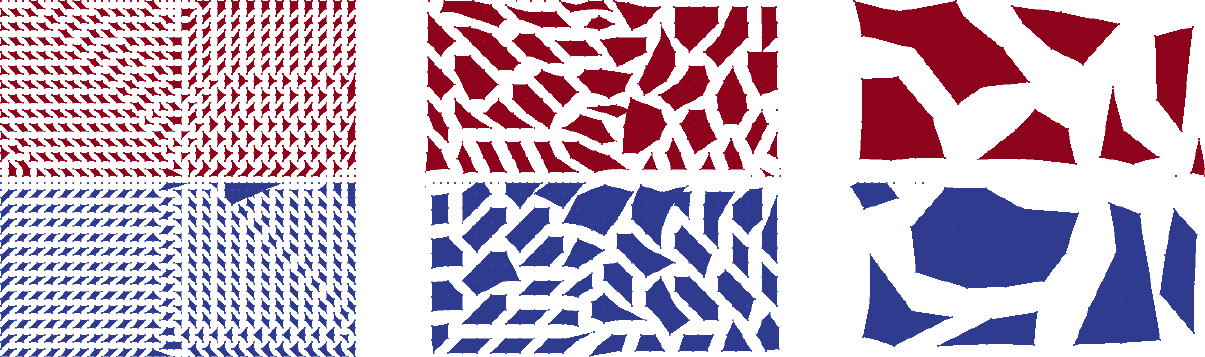
\includegraphics[width=0.7\textwidth]{pics/aggsNonSymm.png}
\caption{Aggregates for Recirc2D example on $50\times 50$ mesh with dropping.}
\label{fig:nonsymAggs}
\end{figure}

\paragraph{Note on coupled aggregation strategy:}
Comparing Figures \ref{fig:symAggs} and \ref{fig:nonsymAggsCoupled} one finds the difference between the \verb|uncoupled| and the \verb|coupled| aggregation method (\texttt{aggregation: type}). For the \verb|coupled| aggregation strategy the aggregates can overlap processor boundaries.
\begin{figure}
\centering
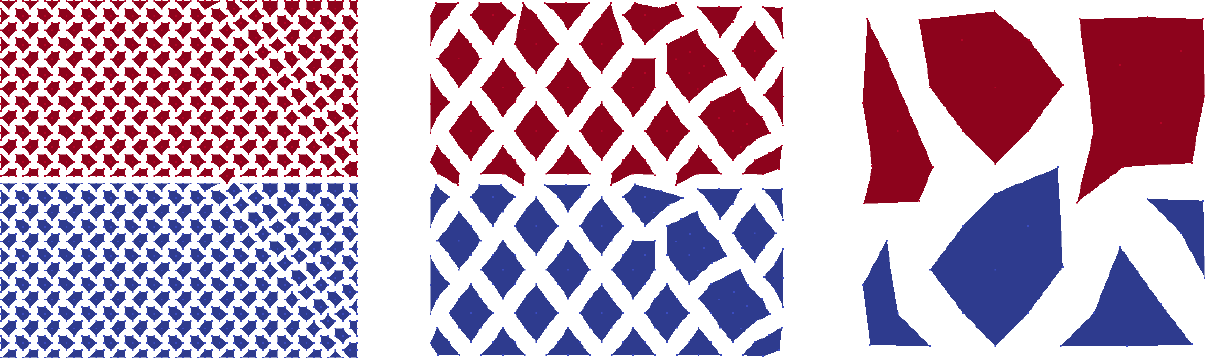
\includegraphics[width=0.7\textwidth]{pics/aggsSymmCoupled.png}
\caption{Aggregates for Laplace2D example on $50\times 50$ mesh without dropping using a coupled aggregation strategy.}
\label{fig:nonsymAggsCoupled}
\end{figure}

\begin{mycomment}
Using the \verb|coupled| aggregation in general is not recommended, since
\begin{itemize}
\item[-] the aggregation routine itself needs some global communication,
\item[-] building the tentative prolongation operator from the aggregates needs some global communication,
\item[-] prolongator smoothing is more expensive due to a higher overlap.
\end{itemize}
The implementation of a \verb|coupled| aggregation method is much more complicated and therefore error-prone and less robust.
\end{mycomment}



\section{Export data}
\label{sec:exportdatasimple}
For debugging purposes it can be very helpful to have a look at the coarse level matrices as well as the transfer operators. \muelu allows to export the corresponding operators to the matrix market format such that the files can be imported, e.g., into MATLAB (or Scilab) for some in-depth analysis.

Using the following xml file writes the fine level operator and the coarse level operator as well as the prolongation and restriction operator to the hard disk using the filenames \texttt{A\_0.m}, \texttt{A\_1.m} as well as \texttt{P\_1.m} and \texttt{R\_1.m}
\lstinputlisting{../src/xml/n2_easy_export.xml}
\begin{mycomment}
Be aware that there is no prolongator and restrictor on the finest level (level 0) since the transfer operators between level $\ell$ and $\ell+1$ are always associated with the coarse level $\ell +1$ (for technical reasons). So, be not confused if there is no \texttt{P\_0.m} and \texttt{R\_0.m}. Only the operators are written to external files which really exist and are requested in the corresponding list in the xml parameters.
\end{mycomment}

The exported files can easily imported into MATLAB and used for some in-depth analysis (determining the eigenvalue spectrum, sparsity pattern,\ldots).

\chapter{Challenge: CD example}

\section{Practical example}

Often one has only very rough information about the linear system that is supposed to be effectively solved using iterative methods with multigrid preconditioners. Therefore, it is highly essential to gain some experience with the solver and preconditioner parameters and learn to optimize the multigrid parameters just by looking at the convergence behavior of the linear solver.

Here, we consider a convection-diffusion example with $16641$ degrees of freedom. No further information is provided (geometry, discretization technique, \ldots).

\section{User-interface}
Run the \verb|hands-on.sh| script and choose the option 4 for the convection-diffusion example. The script automatically generates a XML file with reference multigrid parameters which are far from being optimal.
\begin{center}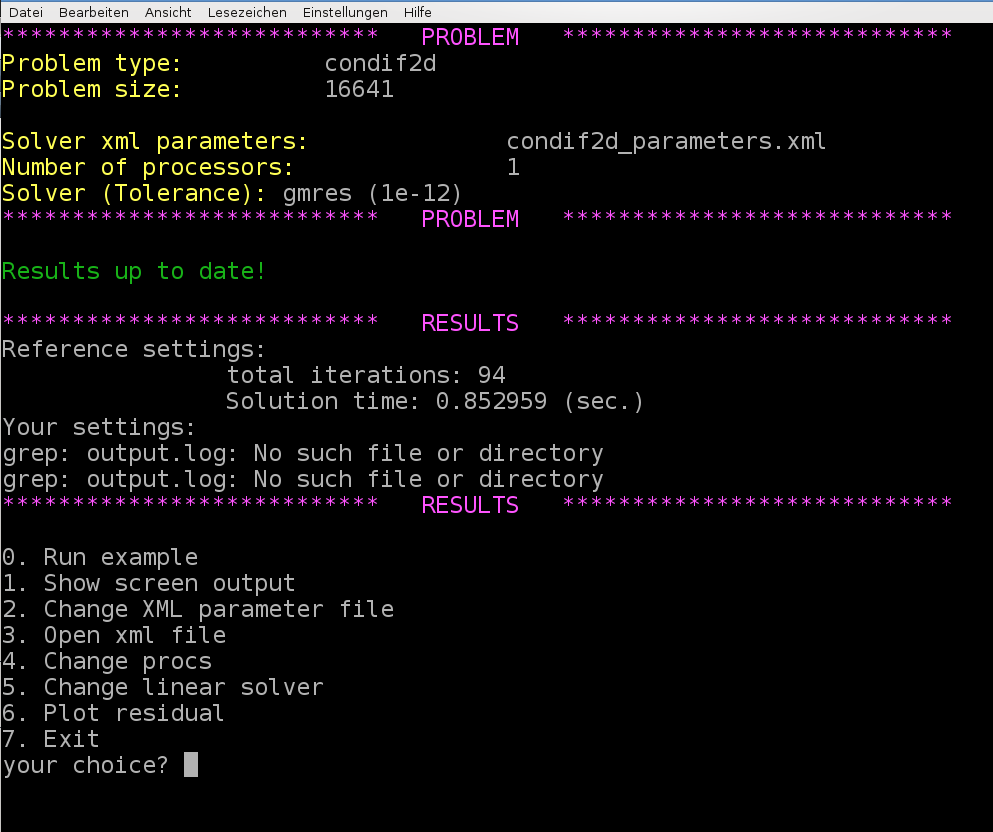
\includegraphics[width=10cm]{pics/tut1_16.png} \end{center}

When using the reference settings for the multigrid preconditioner we need 94 linear iterations. The challenge is to find optimized multigrid settings which results in a significantly lower number of linear iterations and -- even more important -- a lower computational time.

\begin{mycomment}
Please notice that we have automatically chosen GMRES as solver as the linear systems arising from convection-diffusion problems are non-symmetric (due to the convective term). A CG methods would not converge.
\end{mycomment}

\begin{exercise}
Open the \verb|condif2d_parameters.xml| file by pressing option 3. Try to find optimized multigrid settings using your knowledge from the previous tutorials. Save the file and rerun the example (using option 0). Compare your results with the reference results. With option 6 you can plot the convergence of the relative residual of the iterative solver (for comparison).
\end{exercise}

\section{General hints}
\label{sec:generalhings}
There is a very simple strategy for optimizing the solver and preconditioner parameters iteratively that works for many examples surprisingly well.

\subsection{Linear solver settings}
The parameters for the linear solver usually are fixed. Just make sure that you consider the non-symmetry in the choice of your iterative method and choose the solver tolerance in a reasonable way. Before you think about finding good preconditioner parameters you should be absolutely sure that your linear solver is chosen appropriately for your problem.

\subsection{General multigrid settings}
Next, one should choose the multigrid settings. This includes the desired number of multigrid levels and the stopping criterion for the coarsening process. An appropriate choice here is mainly dominated by the size of the problem and the discretization. The multigrid parameters should be chosen such that one obtains a reasonably small problem on the coarsest level which is solved directly.

\subsection{Transfer operators}
Then, one should think about the transfer operators. In the symmetric case one can try smoothed aggregation transfer operators. If unsure, the non-smooth transfer operators always should be a safe and robust starting point.

\subsection{Level smoothers}
Once the multigrid skeleton is fixed by the choice of transfer operators one can start with optimizing the level smoothers. When using relaxation based level smoothers one should first try different smoothing parameters and increase the number of smoothing sweeps only when necessary.

\subsection{Fine tuning}
Sometimes it is very helpful to have a look at the multigrid matrices. 
First of all, one should check whether the aggregation is working properly. This can be done by checking the screen output for the coarsening rate and the aggregation details (this is often the only way to do it if aggregates cannot be visualized due to missing node coordinates). If there is some problem with the aggregation one should try to adapt the aggregation parameters. Here it might make sense to export the coarse level matrices first and study their properties. For finding aggregation parameters one should, e.g., check the number of non-zeros in each row and choose the minimum aggregation size accordingly.

\part{Advanced topics}

\chapter{XML interface for advanced users}

This tutorial introduces the more advanced (and more flexible) XML interface that can be used for setting up multigrid hierarchies in \muelu.
Again we use the 2D Laplace problem on a $50\times 50$ mesh as introduced in \S\ref{lab:examplesym}. That is, in the \verb|hands-on.py| script  you have to choose option 0 for the problem type.


\section{One-level method} 
Before applying a multigrid method as solver, we start with a simple Jacobi iteration as solver and look at the error. By setting the maximum number of multigrid levels to 1 and using a Jacobi smoother as coarse solver we obtain a pseudo multigrid method which corresponds to a simple Jacobi iteration.

\lstinputlisting{../src/xml/s2_adv_a.xml}

The advanced XML format is more hierarchical in the structure. Each XML file in the advanced format consists of two major blocks. First there is a set of ``Factory'' blocks which describe the building blocks within your multigrid methods. In above example there is only one building block specified for the Jacobi method. Each building block needs a (unique) name. In above example the building block has the name \textit{myJacobi}. It is a factory of type \verb|TrilinosSmoother| and describes a damped Jacobi method as declared by the internal parameters.

Later we will see examples for other building blocks describing transfer operators or the aggregation strategy.
In the ``Factories'' list, the user has to declare all building blocks of the multigrid method that are used for the setup. The user cannot specify all building blocks involved in the setup process. \muelu will take care of that and use default building blocks for all parts of the setup process where the user makes no explicit statement. This way the user only has to describe what he explicitly needs.

It is not sufficient just to declare some building blocks. One also has to register them in the setup process. This is done in the second part of the XML file. The so-called \textit{Hierarchy} block describes the setup process. First there are some basic multigrid parameters that are well-known from the easy XML interface (cf. the previous tutorials). Then, there is an additional list of parameters \textit{All} which encapsulates the information which factory block is responsible to provide certain data. In above example you can see, that the building block \textit{myJacobi} shall be used both for the level smoother and the coarse solver. Since it is only a 1 level problem it would be sufficient to define a coarse solver only.
The name of the parameter list \textit{All} can be chosen by the user. It basically describes the user-specified parts of the setup process for all multigrid levels. In this case we just overwrite the internal default factories both for the level smoother and the coarse solver by our Jacobi smoother.
\begin{mycomment}
Be aware that we can have different parameter list sets for different levels, that is, we can use different factories on certain levels.
\end{mycomment}

\begin{exercise}
Run the \verb|hands-on.py| script and choose the XML file \texttt{xml/s2\_adv\_a.xml} which contains above XML parameters. Use only 1 processor and visualize the error for an increasing number of multigrid cycles (e.g. 1, 5, 10, 30, 100). What do you observe?
\end{exercise}
\begin{exercise}
Note that the relaxation based smoothers are based on a Schwarz method (see \ifpack documentation). Repeat above steps using 2 processors. What do you observe in the error plots?
\end{exercise}

\section{Multigrid method} 
The next step is to introduce a full multigrid algorithm. First one should increase the number of multigrid levels. Second, we switch to a direct solver on the coarsest level.\\

\begin{exercise}
Create your own copy of the \texttt{xml/s2\_adv\_a.xml} parameter file. Adapt it to obtain a 3 level multigrid method. Check how this affects the error plots.
\end{exercise}
\begin{exercise}
Change to a direct solver on the coarsest level. You can do this by using \texttt{<Parameter name="CoarseSolver" type="string" value="DirectSolver"/>} in the \textit{Hierarchy} block of the xml file. Check the output of the multigrid hierarchy.
\end{exercise}

\section{Level smoothers} 
Next, we give some building blocks for different types of level smoothers that you can use. Note that all these xml blocks can be put into the \textit{Factories} block of the advanced \muelu XML file format. Then you can use them by adding the corresponding link into the \textit{Hierarchy} block using the name of the parameter block.

\begin{itemize}

\item Chebyshev smoother: 
\begin{lstlisting}
    <ParameterList name="Chebyshev">
      <Parameter name="factory"                     type="string" value="TrilinosSmoother"/>
      <Parameter name="type"                               type="string" value="CHEBYSHEV"/>

      <ParameterList name="ParameterList">
        <Parameter name="chebyshev: degree"                 type="int"     value="2"/>>
        <Parameter name="chebyshev: ratio eigenvalue"       type="double"  value="20"/>
        <Parameter name="chebyshev: min eigenvalue"         type="double"  value="1.0"/>
        <Parameter name="chebyshev: zero starting solution" type="bool"    value="true"/>
      </ParameterList>
    </ParameterList>
\end{lstlisting}
\item Jacobi smoother:
\begin{lstlisting}
    <ParameterList name="myJacobi">
      <Parameter name="factory"                       type="string" value="TrilinosSmoother"/>
      <Parameter name="type"                                type="string" value="RELAXATION"/>
      <ParameterList name="ParameterList">
        <Parameter name="relaxation: type"                  type="string" value="Jacobi"/>
        <Parameter name="relaxation: sweeps"                type="int"    value="1"/>
        <Parameter name="relaxation: damping factor"        type="double" value="0.9"/>
      </ParameterList>
    </ParameterList>   
\end{lstlisting}
\item Gauss--Seidel smoother variants:
\begin{lstlisting}
    <ParameterList name="SymGaussSeidel">
      <Parameter name="factory"                       type="string" value="TrilinosSmoother"/>
      <Parameter name="type"                                type="string" value="RELAXATION"/>
      <ParameterList name="ParameterList">
        <Parameter name="relaxation: type"                  type="string" value="Symmetric Gauss-Seidel"/>
        <Parameter name="relaxation: sweeps"                type="int"    value="1"/>
        <Parameter name="relaxation: damping factor"        type="double" value="1.0"/>
      </ParameterList>
    </ParameterList>
\end{lstlisting}

\begin{lstlisting}
    <ParameterList name="ForwardGaussSeidel">
      <Parameter name="factory"                        type="string" value="TrilinosSmoother"/>
      <Parameter name="type"                                type="string"  value="RELAXATION"/>

      <ParameterList name="ParameterList">
        <Parameter name="relaxation: type"                  type="string"  value="Gauss-Seidel"/>
        <Parameter name="relaxation: backward mode"         type="bool"    value="false"/>
        <Parameter name="relaxation: sweeps"                type="int"     value="2"/>
        <Parameter name="relaxation: damping factor"        type="double"  value="1"/>
      </ParameterList>
    </ParameterList>
\end{lstlisting}

\begin{lstlisting}
    <ParameterList name="BackwardGaussSeidel">
      <Parameter name="factory"                        type="string" value="TrilinosSmoother"/>
      <Parameter name="type"                                type="string"  value="RELAXATION"/>

      <ParameterList name="ParameterList">
        <Parameter name="relaxation: type"                  type="string"  value="Gauss-Seidel"/>
        <Parameter name="relaxation: backward mode"         type="bool"    value="true"/>
        <Parameter name="relaxation: sweeps"                type="int"     value="2"/>
        <Parameter name="relaxation: damping factor"        type="double"  value="1"/>
      </ParameterList>
    </ParameterList>
\end{lstlisting}
\end{itemize}

Beside above level smoothers there are more level smoothers such as ILU methods.\\

\begin{exercise}
Pick out one level smoother from above and use them for your problem. Note that you may have to adapt the \texttt{relaxation: damping factor} for reasonable results.
\end{exercise}

\section{Advanced features} 
\muelu allows full control over the behavior of the multigrid levels. Here, we demonstrate the capabilities of \muelu using the level smoothers.
Take a look at the following example XML parameter list
\lstinputlisting{../src/xml/s2_adv_b.xml}

You can find the parameters in \texttt{xml/s2\_adv\_b.xml}. We have one building block \textit{BackwardGaussSeidel} representing the level smoother that we want to use in our multigrid hierarchy. As one can see from the \textit{Hierarchy} block we request a 4 level multigrid method. There are two blocks called \textit{Finest} and \textit{Remaining} describing the behavior of the different multigrid levels. Note the \texttt{startLevel} parameter in the block \textit{Remaining}. This parameter is missing in the \textit{Finest} block (where it is assumed to be the default value which is zero). That is, in this example we use the backward Gauss--Seidel method as pre-smoother on the finest level (note the keyword \textit{NoFactory} for \texttt{PostSmoother}). The parameter \texttt{startLevel=1} in the \textit{Remaining} block means that for level 1 and all coarser levels (unless there is another block with \texttt{startLevel > 1}) the building blocks from \textit{Remaining} shall be used for the multigrid setup. That is, on the multigrid levels 1 and 2 the backward Gauss--Seidel method is used for post smoothing only. The corresponding multigrid hierarchy has the form
\printScreenOutput{s2_adv_b.txt_3.fragment_3.fragment}

\begin{exercise}
  Create an XML file in advanced format which produces the following multigrid layout
  \printScreenOutput{s2_adv_c.txt_3.fragment_3.fragment}. 
  
  Hint: create a copy of the file \texttt{xml/s2\_adv\_b.xml} and extend it accordingly. A possible solution can be found in \texttt{xml/s2\_adv\_c.xml}.
\end{exercise}


\chapter{\muelu factories for transfer operators}

For this example we reuse the \verb|Recirc2D| example as introduced in \S\ref{sec:recircexample}. The resulting linear systems are (slightly) non-symmetric and classical smoothed aggregation methods may be able to solve the problem but are not optimal in sense of convergence.

\section{Multigrid setup phase -- algorithmic design}

Smoothed aggregation based algebraic multigrid methods originally have not been designed for non-symmetric linear systems. Inappropriately smoothed transfer operators may significantly deteriorate the convergence rate or even break convergence completely.

\subsection{Unsmoothed transfer operators}
Before we introduce smoothed aggregation methods for non-symmetric linear systems we first go back one step and demonstrate how to use non-smoothed transfer operators which are eligible for non-symmetric linear systems. Figure \ref{fig:simpledesignnonsmoothed} gives a simplified example how to build the coarse level matrix $A_c$ using the fine level matrix $A$ only. First, we ``somehow'' build aggregates using the information of the fine level matrix $A$. The aggregates are then used to build the tentative non-smoothed prolongation operator. The restrictor is just the transpose of the (tentative) prolongator and finally the coarse level matrix $A_c$ is calculated by the triple product $A_c=RAP$.

In Figure \ref{fig:simpledesignsaamg} the \verb|SaPFactory| has been added after the \verb|TentativePFactory|. Therein the non-smoothed transfer operator from the \verb|TentativePFactory| is smoothed using information of the fine level matrix $A$. This transfer operator design is used per default when the user does not specify its own transfer operator design. The default settings are optimal for symmetric positive definite systems. However for our non-symmetric problem they might be problematic.

\begin{figure}
\subfigure[Non-smoothed aggregation based AMG\label{fig:simpledesignnonsmoothed}]{
\scalebox{0.5}{
\begin{tikzpicture}[>=latex',font={\sf \small}, node distance=2cm]
\def\datawidth{2cm}
\def\dataheight{0.5cm}
\def\factorywidth{4cm}
\def\factoryheight{0.75cm}
%\draw[help lines] (-10,-10) grid (10,10);
\begin{scope}[>=triangle 60]
\node(A) at (-3,10) [draw, terminal, minimum width=\datawidth, minimum height=\dataheight]{$A$};
\node(nothing) at (-3,8) [draw, process, minimum width=\factorywidth, minimum height=\factoryheight]{...};
\node [draw, process, minimum width=\factorywidth, minimum height=\factoryheight, below of=nothing] (AggregationFactory) {AggregationFactory};
\node [draw, process, minimum width=\factorywidth, minimum height=\factoryheight, below of=AggregationFactory] (TentativePFactory) {TentativePFactory};
\node [draw, process, minimum width=\factorywidth, minimum height=\factoryheight, right of=TentativePFactory,node distance=6cm] (TransPFactory) {TransPFactory};
\node [draw, process, minimum width=\factorywidth, minimum height=\factoryheight, below of=TentativePFactory] (RAPFactory) {RAPFactory};
\node(A2) at (-3,0) [draw, terminal, minimum width=\datawidth, minimum height=\dataheight]{$A_c$};
\draw[->] (A) -- (nothing);
\draw[->] (nothing) -- (AggregationFactory);
\draw[->] (A) to[out=180,in=180] node [near start, left] {} (TentativePFactory);
\draw[->] (A) to[out=180,in=180] node [near start, left] {} (RAPFactory);
\draw[->] (AggregationFactory) -- node [near start, left] {Aggregates} (TentativePFactory);
\draw[->] (TentativePFactory) -- node [near start, below] {P} (TransPFactory);
\draw[->] (TentativePFactory) -- node [near start, left] {P} (RAPFactory);
\draw[->] (TransPFactory) -- node [near start, below] {R} (RAPFactory);
\draw[->] (RAPFactory) -- node [near start, below] {} (A2);
\end{scope}
\end{tikzpicture}
} % end scalebox
} % end subfigure 1
\subfigure[Smoothed aggregation AMG (SA-AMG)\label{fig:simpledesignsaamg}]{
\scalebox{0.5}{
\begin{tikzpicture}[>=latex',font={\sf \small}, node distance=2cm]
\def\datawidth{2cm}
\def\dataheight{0.5cm}
\def\factorywidth{4cm}
\def\factoryheight{0.75cm}
%\draw[help lines] (-10,-10) grid (10,10);
\begin{scope}[>=triangle 60]
\node(A) at (-3,10) [draw, terminal, minimum width=\datawidth, minimum height=\dataheight]{$A$};
\node(nothing) at (-3,8) [draw, process, minimum width=\factorywidth, minimum height=\factoryheight]{...};
\node [draw, process, minimum width=\factorywidth, minimum height=\factoryheight, below of=nothing] (AggregationFactory) {AggregationFactory};
\node [draw, process, minimum width=\factorywidth, minimum height=\factoryheight, below of=AggregationFactory] (TentativePFactory) {TentativePFactory};
\node [draw, process, minimum width=\factorywidth, minimum height=\factoryheight, below of=TentativePFactory] (SaPFactory) {SaPFactory};
\node [draw, process, minimum width=\factorywidth, minimum height=\factoryheight, right of=SaPFactory,node distance=6cm] (TransPFactory) {TransPFactory};
\node [draw, process, minimum width=\factorywidth, minimum height=\factoryheight, below of=SaPFactory] (RAPFactory) {RAPFactory};
\node(A2) at (-3,-2) [draw, terminal, minimum width=\datawidth, minimum height=\dataheight]{$A_c$};
\draw[->] (A) -- (nothing);
\draw[->] (nothing) -- (AggregationFactory);
\draw[->] (A) to[out=180,in=180] node [near start, left] {} (TentativePFactory);
\draw[->] (A) to[out=180,in=180] node [near start, left] {} (SaPFactory);
\draw[->] (A) to[out=180,in=180] node [near start, left] {} (RAPFactory);
\draw[->] (AggregationFactory) -- node [near start, left] {Aggregates} (TentativePFactory);
\draw[->] (TentativePFactory) -- node [near start, left] {P} (SaPFactory);
\draw[->] (SaPFactory) -- node [near start, below] {P} (TransPFactory);
\draw[->] (SaPFactory) -- node [near start, left] {P} (RAPFactory);
\draw[->] (TransPFactory) -- node [near start, below] {R} (RAPFactory);
\draw[->] (RAPFactory) -- node [near start, below] {} (A2);
\end{scope}
\end{tikzpicture}
} % end scalebox
} % end subfigure 2
\caption{Simple factory design for aggregation based algebraic multigrid methods.}
\label{fig:simpledesign}
\end{figure}


\subsection{Smoothed transfer operators for non-symmetric systems}
In case of non-symmetric linear systems it is $A\neq A^T$. Therefore it is a bad idea just to use the transposed of the smoothed prolongation operator for the restrictor. Let $\widehat{P}$ be the non-smoothed tentative prolongation operator. Then the smoothed prolongation operator $P$ is built using
\begin{displaymath}
P = \bigl(I-\omega A\bigr) \widehat{P},
\end{displaymath}
with some reasonable smoothing parameter $\omega>0$.
The standard restrictor is
\begin{displaymath}
R = P^T = \widehat{P}^T - \omega \widehat{P}^T A^T = \widehat{P}^T\bigl(I-\omega A^T\bigr).
\end{displaymath}
That is, the restrictor would be smoothed using the information of $A^T$. However, for non-symmetric systems we want to use the information of matrix $A$ for smoothing the restriction operator, too. The restriction operator shall we built by the formula
\begin{displaymath}
R = P^T = \widehat{P}^T - \omega \widehat{P}^T A.
\end{displaymath}
This corresponds to apply the same smoothing strategy to the non-smoothed restriction operator $\widehat{R}=\widehat{P}^T$ which is applied to the (tentative) prolongation operator with using $A^T$ as input instead of matrix $A$. Figure \ref{fig:simpledesignpgamg} shows the changed factory design. The dashed line denotes, that the same smoothing strategy is used than for the prolongation operator. The concept is known as Petrov-Galerkin smoothed aggregation approach in the literature.
A more advanced transfer operator smoothing strategy for non-symmetric linear systems that is based on the Petrov-Galerkin approach is described in \cite{sala2008}. Another approach based on SchurComplement approximations can be found in \cite{wiesner2013}.

\begin{figure}
\begin{center}
\scalebox{0.5}{
\begin{tikzpicture}[>=latex',font={\sf \small}, node distance=2cm]
\def\datawidth{2cm}
\def\dataheight{0.5cm}
\def\factorywidth{4cm}
\def\factoryheight{0.75cm}
%\draw[help lines] (-10,-10) grid (10,10);
\begin{scope}[>=triangle 60]
\node(A) at (-3,10) [draw, terminal, minimum width=\datawidth, minimum height=\dataheight]{$A$};
\node(nothing) at (-3,8) [draw, process, minimum width=\factorywidth, minimum height=\factoryheight]{...};
\node [draw, process, minimum width=\factorywidth, minimum height=\factoryheight, below of=nothing] (AggregationFactory) {AggregationFactory};
\node [draw, process, minimum width=\factorywidth, minimum height=\factoryheight, below of=AggregationFactory] (TentativePFactory) {TentativePFactory};
\node [draw, process, minimum width=\factorywidth, minimum height=\factoryheight, below of=TentativePFactory] (SaPFactory) {SaPFactory};
\node [draw, process, minimum width=\factorywidth, minimum height=\factoryheight, right of=SaPFactory,node distance=6cm] (GenericRFactory) {GenericRFactory};
\node [draw, process, minimum width=\factorywidth, minimum height=\factoryheight, below of=SaPFactory] (RAPFactory) {RAPFactory};
\node(A2) at (-3,-2) [draw, terminal, minimum width=\datawidth, minimum height=\dataheight]{$A_c$};
\draw[->] (A) -- (nothing);
\draw[->] (nothing) -- (AggregationFactory);
\draw[->] (A) to[out=180,in=180] node [near start, left] {} (TentativePFactory);
\draw[->] (A) to[out=180,in=180] node [near start, left] {} (SaPFactory);
\draw[->] (A) to[out=180,in=180] node [near start, left] {} (RAPFactory);
\draw[->] (A) to[out=0,in=90] node [near end, right] {$A^T$} (GenericRFactory);
\draw[->] (AggregationFactory) -- node [near start, left] {Aggregates} (TentativePFactory);
\draw[->] (TentativePFactory) -- node [near start, left] {P} (SaPFactory);
\draw[->,dashed] (SaPFactory) -- node [near start, below] {} (GenericRFactory);
\draw[->] (SaPFactory) -- node [near start, left] {P} (RAPFactory);
\draw[->] (GenericRFactory) -- node [near start, below] {R} (RAPFactory);
\draw[->] (RAPFactory) -- node [near start, below] {} (A2);
\end{scope}
\end{tikzpicture}
} % end scalebox
\end{center}
\caption{Simple factory design for smoothed aggregation based algebraic multigrid methods for non-symmetric systems.}
\label{fig:simpledesignpgamg}
\end{figure}

\section{XML interface}

\subsection{Unsmoothed transfer operators} 
To construct a multigrid hierarchy with unsmoothed transfer operators one can use the following XML file (stored in \texttt{xml/s3a.xml})

\lstinputlisting{../src/xml/s3a.xml}

Beside the \verb|TentativePFactory| which is responsible to generate the unsmoothed transfer operators we also introduce the \verb|UncoupledAggregationFactory| with this example. In the \textit{Factories} section of the XML file you find both an entry for the aggregation factory and the prolongation operator factory with its parameters. In the \textit{Hierarchy} section the defined factories are just put in into the multigrid setup algorithm. That is, the factory with the name \verb|UncoupledAggregationFact| is used to generate the \verb|Aggregates| and the \verb|myTentativePFact| is responsible for generating both the (unsmoothed) prolongation operator \verb|P| and the (coarse) near null space vectors \verb|Nullspace|.\\

\begin{mycomment}
Be aware that it is highly important not to forget to register the \verb|myTentativePFact| object for generating null space \verb|Nullspace|. It is not visualized in the dependency trees, but the \verb|TenativePFactory| factory both generates the unsmoothed prolongation operator and the set of near null space vectors for the coarse level. So, if you declare your own explicit instance of a \verb|TentativePFactory| you always have to register it for the near null space, too. In general it is a good idea to register a factory in the \textit{Hierarchy} sublist for all output variables of the factory.
\end{mycomment}

\begin{mycomment}
Note that one can also use the \verb|Ptent| variable for registering a \verb|TentativePFactory|. This makes the \verb|TentativePFactory| somewhat special in its central role for generating an aggregation based multigrid hierarchy. \muelu is smart enough to understand that you want to use the near null space vectors generated by the factory registered as \verb|Ptent| for setting up the transfer operators.

That is, the following code would explicitly use the \verb|TentativePFactory| object that is created as \verb|myTentativePFact|. Since no factory is specified for the prolongation operator \verb|P| \muelu would decide to use a smoothed aggregation prolongation operator (represented by the \verb|SaPFactory|) which correctly uses the factory for \verb|Ptent| for the unsmoothed transfers with all its dependencies.
\begin{lstlisting}
<ParameterList name="MueLu">
  <ParameterList name="Factories">   
    <ParameterList name="myTentativePFact">
      <Parameter name="factory"   type="string" value="TentativePFactory"/>
    </ParameterList>
  </ParameterList>

  <ParameterList name="Hierarchy">
    <ParameterList name="Levels">
      <Parameter name="Ptent"     type="string" value="myTentativePFact"/>
    </ParameterList>
  </ParameterList>
</ParameterList>
\end{lstlisting}

\end{mycomment}

\begin{exercise}
  Create a sublist in the \textit{Factories} part of the XML file for the restriction operator factory. Use a \verb|TransPFactory| which builds the transposed of \verb|P| to generate the restriction operator \verb|R|. Register your restriction factory in the \textit{Hierarchy} section to generate the variable \verb|R|.
\end{exercise}

\subsection{Smoothed aggregation for non-symmetric problems}

Next, let's try smoothed transfer operators for the non-symmetric linear system and compare the results of the transfer operator designs. Take a look at the XML file (in \texttt{xml/s3b.xml}).

\lstinputlisting{../src/xml/s3b.xml}

The interesting part is the \textit{Factories} section where several different factories for the restriction operator are defined
\begin{description}
\item[\textit{myTentRestrictorFact:}] just uses the transposed of the unsmoothed prolongator for restriction.
\item[\textit{mySymRestrictorFact:}] uses the transposed of the smoothed prolongator for restriction.
\item[\textit{myNonsymRestrictorFact:}] uses the special non-symmetric smoothing for the restriction operator (based on the \verb|SaPFactory| smoothing factory).
\end{description}

\begin{mycomment}
The \muelu framework is very flexible and allows for arbitrary combinations of factories. However, be aware that the \verb|TentativePFactory| cannot be used as input for the \verb|GenericRFactory|. That is no problem since this combination not really makes sense. If you are using the \verb|TentativePFactory| as your final prolongation operator you always have to use the \verb|TransPFactory| for generating the restriction operators.
\end{mycomment}

\begin{exercise}
Run the \verb|Recirc2D| example with the different restriction operator strategies and compare the results for the iterative solver. What do you observe? What is the best choice for the transfer operators in the non-symmetric case?
\end{exercise}
\begin{exercise}
Change the \verb|myProlongatorFact| from type \verb|SaPFactory| to \verb|PgPFactory| which uses automatically calculated local damping factors instead of a global damping factor (with some user parameter \texttt{sa: damping factor}). Note that the \verb|PgPFactory| might not accept the \verb|sa: damping factor| parameter such that you have to comment it out (using \texttt{<!-- ... -->}).
\end{exercise}
\begin{exercise}
Try to set up a multigrid hierarchy with unsmoothed transfer operators for the transition from the finest level to level 1 and then use smoothed aggregation for the coarser levels (starting from level 1).
\end{exercise}

% results
%\printScreenOutput{s3b1.txt_5.fragment}
%\printScreenOutput{s3b2.txt_5.fragment}
%\printScreenOutput{s3b3.txt_5.fragment}

\chapter{Rebalancing - Hypergraph repartitioning}

\section{Basic concepts and parameters}
It's a natural thing to use lesser processors for the coarse level problem than for the fine level problem. This is an elegant way to avoid the problems of the coupled aggregation strategy, by just using the uncoupled aggregation strategy with rebalancing on the coarser levels.

In this tutorial we use a hypergraph based repartitioning for the coarse level matrices $A_c$ to rebalance the problem. The repartitioning algorithm is implemented in the \zoltan package of \trilinos. The advantage of the hypergraph based repartitioning methods is, that they do not need additional information such as node coordinates and therefore are the consequent choice within algebraic multigrid preconditioners.

\begin{mycomment}
Hypergraph partitioning algorithms as PHG are not available in the new \zoltantwo package of \trilinos, yet. Therefore we can use this type of repartitioning only in context of \epetra based applications. If you use the new templated \tpetra stack you have to use repartitioning algorithms which are available in \zoltantwo such as RCB.
\end{mycomment}

Repartitioning algorithms are a very wide field of research and can be very complicated. Here, we cannot go into details and just focus on how to use them. Basically there are only a few really important parameters that the user has to set properly:
\begin{description}
\item \texttt{repartition: min rows per proc} the minimum number of rows each processor shall handle. This parameter is used to reduce the number of involved processors on the coarser levels. If for example the parameter value is chosen to be 1000 and the fine level problem has 10000 rows whereas the coarse level problem has 2000 rows, then the fine level problem is solved on not more than 10 processors at maximum and for the coarse level problem there are not more processors than at maximum 2 being used.
\item \texttt{repartition: max imbalance} This parameter defines the maximum allowed imbalance ratio of nonzeros on all processors. If the value is set to 1.2, and there is one processor with more than 20\% nonzeros compared to another processor, than the problem will be rebalanced.
\item \texttt{repartition: start level} start rebalancing on given level and coarser levels. This allows to avoid the costs of rebalancing on the finer levels (where it is not really necessary).
\end{description}

\section{Transfer operator design}

Figure \ref{fig:rebalanceddesignpgamg} gives the extended factory design for smoothed aggregation based AMG for non-symmetric linear systems with rebalancing enabled. Nothing has changed in the upper part where the non-rebalanced Galerkin product has been calculated using the \verb|RAPFactory|. The coarse level matrix $A_c$ as output from the \verb|RAPFactory| then is checked for its partition and rebalanced.

The \verb|AmalgamationFactory| amalgamates the matrix, i.e. it generates some mapping between the actual degrees of freedom and the corresponding nodes or supernodes. In fact the \verb|AmalgamationFactory| is only important if there are more than one degree of freedom per node. Otherwise the mappings are trivial to build.

The \verb|IsorropiaInterface| class first builds internally the graph of the coarse level matrix $A_c$ using the information from the \verb|AmalgamationInformation| and then calls the repartitioning algorithm from \zoltan through the \isorropia interface\footnote{\isorropia is a \trilinos package which provides an easy-to-use interface to many partitioning algorithms in \zoltan.}. The output is an amalgamated repartitioning information. Then the \verb|RepartitionInterface| factory resembles the un-amalgamated repartitioning information which is put into the \verb|RepartitionFactory|.

The \verb|RepartitionFactory| is the most important factory and responsible for the repartitioning. Therein the decision is made whether repartitioning is necessary at all. It creates the communication ``plan'' that is used to rebalance the transfer operators and the coarse level matrix.

\begin{figure}
\begin{center}
\scalebox{0.8}{
\begin{tikzpicture}[>=latex',font={\sf \small}, node distance=2cm]
\def\datawidth{2cm}
\def\dataheight{0.5cm}
\def\factorywidth{4cm}
\def\factoryheight{0.75cm}
%\draw[help lines] (-10,-10) grid (10,10);
\begin{scope}[>=triangle 60]
\node(A) at (0,10) [draw, terminal, minimum width=\datawidth, minimum height=\dataheight]{$A$};
\node(nothing) at (-3,8) [draw, process, minimum width=\factorywidth, minimum height=\factoryheight]{...};
\node [draw, process, minimum width=\factorywidth, minimum height=\factoryheight, below of=nothing] (AggregationFactory) {AggregationFactory};
\node [draw, process, minimum width=\factorywidth, minimum height=\factoryheight, below of=AggregationFactory] (TentativePFactory) {TentativePFactory};
\node [draw, process, minimum width=\factorywidth, minimum height=\factoryheight, below of=TentativePFactory] (SaPFactory) {PgPFactory};
\node [draw, process, minimum width=\factorywidth, minimum height=\factoryheight, right of=SaPFactory,node distance=6cm] (GenericRFactory) {GenericRFactory};
\node(RAPFactory) at(0,0) [draw, process, minimum width=\factorywidth, minimum height=\factoryheight]  {RAPFactory};

\node [draw, process, minimum width=\factorywidth, minimum height=\factoryheight, below of=RAPFactory] (RebAmalgFactory) {AmalgamationFactory};
\node [draw, process, minimum width=\factorywidth, minimum height=\factoryheight, below of=RebAmalgFactory] (IsorropiaInterface) {IsorropiaInterface};
\node [draw, process, minimum width=\factorywidth, minimum height=\factoryheight, below of=IsorropiaInterface] (RepartitionInterface) {RepartitionInterface};
\node [draw, process, minimum width=\factorywidth, minimum height=\factoryheight, below of=RepartitionInterface] (RepartitionFactory) {RepartitionFactory};
\node(RebalanceTransferFactory) at(-3,-10) [draw, process, minimum width=\factorywidth, minimum height=\factoryheight]  {RebalanceTransferFactory};
\node [draw, process, minimum width=\factorywidth, minimum height=\factoryheight, right of=RebalanceTransferFactory,node distance=6cm] (RebalanceTransferFactory2) {RebalanceTransferFactory};
\node(RebalanceAcFactory) at (0,-12) [draw, process, minimum width=\factorywidth, minimum height=\factoryheight]  {RebalanceAcFactory};

\node(A2) at (0,-14) [draw, terminal, minimum width=\datawidth, minimum height=\dataheight]{$A_c$};
\node(P2) [draw, terminal, minimum width=\datawidth, minimum height=\dataheight,node distance=3cm, left of=A2]{$P$};
\node(R2) [draw, terminal, minimum width=\datawidth, minimum height=\dataheight,node distance=3cm, right of=A2]{$R$};
\draw[->] (A) -- (nothing);
\draw[->] (nothing) -- (AggregationFactory);
\draw[->] (A) to[out=270,in=25] node [near start, left] {} (TentativePFactory);
\draw[->] (A) to[out=270,in=25] node [near start, left] {} (SaPFactory);
\draw[->] (A) to[out=270,in=90] node [near start, left] {} (RAPFactory);
\draw[->] (A) to[out=0,in=90] node [near end, right] {$A^T$} (GenericRFactory);
\draw[->] (AggregationFactory) -- node [near start, left] {Aggregates} (TentativePFactory);
\draw[->] (TentativePFactory) -- node [near start, left] {P} (SaPFactory);
\draw[->,dashed] (SaPFactory) -- node [near start, below] {} (GenericRFactory);
\draw[->] (SaPFactory) -- node [near start, below] {P} (RAPFactory);
\draw[->] (GenericRFactory) -- node [near start, below] {R} (RAPFactory);
%\draw[->] (RAPFactory) -- node [near start, below] {} (A2);
\draw[->] (RAPFactory) -- node [near start, left] {$A_c$} (RebAmalgFactory);
\draw[->] (RAPFactory) to[out=190,in=180] node [near end, left] {$A_c$} (IsorropiaInterface);
\draw[->] (RAPFactory) to[out=190,in=180] node [near end, left] {$A_c$} (RepartitionInterface);
\draw[->] (RAPFactory) to[out=190,in=180] node [near end, left] {$A_c$} (RepartitionFactory);
%\draw[->] (RAPFactory) to[out=190,in=180] node [near end, left] {$A_c$} (RebalanceAcFactory);
\draw[->] (RebAmalgFactory) -- node [near start, left] {UnAmalg.Info} (IsorropiaInterface);
\draw[->] (RebAmalgFactory) to[out=0,in=0] node [near start, right] {UnAmalg.Info} (RepartitionInterface);
\draw[->] (IsorropiaInterface) -- node [near start, left] {Amalg.Partition} (RepartitionInterface);
\draw[->] (RepartitionInterface) -- node [near start, left] {Partition} (RepartitionFactory);
\draw[->] (RepartitionFactory) -- node [near start, left] {Importer} (RebalanceTransferFactory);
\draw[->] (RepartitionFactory) -- node [near start, right] {Importer} (RebalanceTransferFactory2);
\draw[->] (RepartitionFactory) -- node [near end, left] {Importer} (RebalanceAcFactory);
\draw[->] (RebalanceAcFactory) -- node [near end, left] {} (A2);
\draw[->] (SaPFactory) to[out=230,in=130] node [near end, left] {P} (RebalanceTransferFactory);
\draw[->] (GenericRFactory) to[out=310,in=50] node [near end, left] {R} (RebalanceTransferFactory2);
\draw[->] (RebalanceTransferFactory) -- (P2);
\draw[->] (RebalanceTransferFactory2) -- (R2);
\end{scope}
\end{tikzpicture}
} % end scalebox
\end{center}
\caption{Factory design for smoothed aggregation based algebraic multigrid methods for non-symmetric systems with rebalancing.}
\label{fig:rebalanceddesignpgamg}
\end{figure}

\section{XML interface}
The corresponding XML parameter file looks as 

\lstinputlisting{../src/xml/s5a.xml}

It is stored in \texttt{xml/s5a.xml}. In this example we define a smoothed aggregation transfer operator strategy (using the \verb|PgPFactory|) for non-symmetric systems. The level smoother is chosen to be an over-relaxed symmetric Gauss--Seidel method. A direct solver is applied on the coarsest level. Please compare the building blocks in the xml file with Figure \ref{fig:rebalanceddesignpgamg}. Be aware that the \textit{Nullspace} variable now is also generated by the \texttt{myRebalanceProlongatorFact}.

\begin{exercise}
Choose option 1 in the problem menu of \verb|hands-on.py| to run the \verb|Laplace 2D| example on a $300\times 300$ mesh.
Change the solver to \verb|xml/s5a.xml|.
Use a reasonable number of processors. For demonstration purposes 4 processors should be fine for the $300\times 300$ mesh.
Run the example and check the screen output to see the effect of rebalancing. Try to visualize the ownership of the aggregates.
\begin{mycomment}
The XML parameters in \verb|xml/s5a.xml| write out the aggregation data for debugging. See the next tutorial for some more background information on aggregation and debugging.
\end{mycomment}
\end{exercise}

You should observe a multigrid hierarchy as follows

\printScreenOutput{s5a.txt_3.fragment_3.fragment}

\chapter{Aggregation}

This tutorial provides some background information about the aggregation process in \muelu. A very detailed description of the aggregation algorithms with all internal details can be found in \cite[Chapter 3.3]{wiesner2014}.

\section{Building aggregates}

The aggregates are built using the graph of the fine level matrix $A$. The graph is generated by the \verb|CoalesceDropFactory|. Since we still only restrict ourselves to scalar problems with one degree of freedom per node (\texttt{DofsPerNode=1}), the graph of the fine level matrix is trivial to build.
Figure \ref{fig:simpledesignaggregates} shows the extended transfer operator design with the additional \verb|CoalesceDropFactory|.

\begin{figure}
\begin{center}
\scalebox{0.6}{
\begin{tikzpicture}[>=latex',font={\sf \small}, node distance=2cm]
\def\datawidth{2cm}
\def\dataheight{0.5cm}
\def\factorywidth{4cm}
\def\factoryheight{0.75cm}
%\draw[help lines] (-10,-10) grid (10,10);
\begin{scope}[>=triangle 60]
\node(A) at (-3,10) [draw, terminal, minimum width=\datawidth, minimum height=\dataheight]{$A$};
\node(CoalesceDropFactory) at (-3,8) [draw, process, minimum width=\factorywidth, minimum height=\factoryheight]{CoalesceDropFactory};
\node [draw, process, minimum width=\factorywidth, minimum height=\factoryheight, below of=nothing] (AggregationFactory) {AggregationFactory};
\node [draw, process, minimum width=\factorywidth, minimum height=\factoryheight, below of=AggregationFactory] (TentativePFactory) {TentativePFactory};
\node [draw, process, minimum width=\factorywidth, minimum height=\factoryheight, below of=TentativePFactory] (SaPFactory) {SaPFactory};
\node [draw, process, minimum width=\factorywidth, minimum height=\factoryheight, right of=SaPFactory,node distance=6cm] (TransPFactory) {TransPFactory};
\node [draw, process, minimum width=\factorywidth, minimum height=\factoryheight, below of=SaPFactory] (RAPFactory) {RAPFactory};
\node [draw, process, minimum width=\factorywidth, minimum height=\factoryheight, right of=RAPFactory,node distance=9cm] (AggExportFactory) {AggregationExportFactory};
\node(A2) at (-3,-2) [draw, terminal, minimum width=\datawidth, minimum height=\dataheight]{$A_c$};
\draw[->] (A) -- (CoalesceDropFactory);
\draw[->] (CoalesceDropFactory) -- node [near start, left] {Graph} (AggregationFactory);
\draw[->] (A) to[out=180,in=180] node [near start, left] {} (TentativePFactory);
\draw[->] (A) to[out=180,in=180] node [near start, left] {} (SaPFactory);
\draw[->] (A) to[out=180,in=180] node [near start, left] {} (RAPFactory);
\draw[->] (AggregationFactory) -- node [near start, left] {Aggregates} (TentativePFactory);
\draw[->] (TentativePFactory) -- node [near start, left] {P} (SaPFactory);
\draw[->] (SaPFactory) -- node [near start, below] {} (TransPFactory);
\draw[->] (SaPFactory) -- node [near start, left] {P} (RAPFactory);
\draw[->] (TransPFactory) -- node [near start, below] {R} (RAPFactory);
\draw[->] (RAPFactory) -- node [near start, below] {} (A2);
\draw[o->] (RAPFactory) -- (AggExportFactory);
\draw[->] (AggregationFactory) to[out=0,in=100] node [near start, right] {Aggregates} (AggExportFactory);
\draw[->] (CoalesceDropFactory) to[out=0,in=80] node [near start, right] {DofsPerNode} (AggExportFactory);
\end{scope}
\end{tikzpicture}
} % end scalebox
\end{center}
\caption{Simple factory design for building aggregates.}
\label{fig:simpledesignaggregates}
\end{figure}


Especially for anisotropic or non-symmetric problems it may be advantageous to drop small entries from the graph of $A$ and use a filtered graph for generating aggregates.

The following listing shows the definition of the \verb|myCoalesceDropFactory| which drops all values of the fine level matrix $A$ with the absolute value smaller than $0.01$. Of course, the \verb|myCoalesceDropFactory| has to be registered to generate the variable \verb|Graph|, which is used by the aggregation factory. 
The \verb|Graph| and the variable \verb|DofsPerNode| generated by the \verb|myCoalesceDropFactory| are needed as input by the \verb|UncoupledAggregationFact|. Note that the aggregation routine always works on the node-based information instead of DOF-based information. Therefore, we first have to build the graph of $A$ which then can be processed by the aggregation algorithm.

\lstinputlisting{../src/xml/s4a.xml}

The listing shows how the \verb|Graph| and the variable \verb|DofsPerNode| generated by the coalescing factory \verb|myCoalesceDropFact| are explicitly used as input for the aggregation routine. This is an example for a direct link of variables from output to the corresponding input. In addition, the \verb|myCoalesceDropFact| is registered to produce the variable \verb|Graph| in the \textit{Hierarchy} section of the XML file. One should also register \verb|myCoalesceDropFact| to produce the \verb|DofsPerNode| information. In our case it is not really necessary, since all factories which rely on information from \verb|DofsPerNode| get the information directly in the XML file (see also \verb|myAggExportFact| in above listing). So, one has in general two possibilities to declare inter-factory dependencies. One can either explicitly describe the input for each factory (as demonstrated for the \verb|Graph| in \verb|UncoupledAggregationFact|) or use the default factories (provided either by \muelu or explicitly set by the user in the \textit{Hierarchy} section). \muelu uses the following ordering: first, the explicit input dependencies within the factories are used by \muelu. If a user does not define input variables (e.g., there is no input for \verb|Aggregates| in \verb|myTentativePFact|), \muelu checks whether there is a default factory for the data variable set in the \textit{Hierarchy} section (in above listing it will find \verb|UncoupledAggregationFact| to be responsible to provide the \verb|Aggregates|). Otherwise \muelu will use some internal default factory.

For demonstration purposes we also introduced a \verb|RAPFactory| which makes use of the user-defined transfer factories \verb|myProlongatorFact| as well as \verb|myRestrictorFact|. The full XML file can be found in \verb|xml/s4a.xml|.\\



\section{Visualization of aggregates}

For debugging purposes it can be very useful to visualize the aggregates. In \muelu there is a helper factory named \verb|AggregationExportFactory| which can be used to export the aggregates for visualization purposes.

The \verb|AggregationExportFactory| acts as a small helper factory within the \verb|RAPFactory| which writes out some aggregation information to files on the hard disk (see figure \ref{fig:simpledesignaggregates}). In a post-processing step one can use these files together with some mesh information to generate pictures of the aggregates on each level. For post-processing we use the \verb|MueLu_Agg2VTK.py| python script which is stored in the \texttt{src} folder of this tutorial. It works both for 2D and 3D problems. You have to provide the output files from the \verb|AggregationExportFactory| as well as a list of node coordinates, that are needed to produce the output in the vtk format which can be opened in paraview.

\begin{mycomment}
The visualization script has successfully been tested with VTK 5.x. Note that it is not compatible to VTK 6.x.
\end{mycomment}

\begin{exercise}
Run the \verb|Laplace 2D| example on a $50\times 50$ mesh using the XML file \verb|xml/s4a.xml|. Visualize the aggregates.
\end{exercise}
\begin{exercise}
In the \verb|xml/s4a.xml| file an uncoupled aggregation factory has been explicitly defined using with some user-chosen aggregation parameters. Make a copy of \verb|xml/s4a.xml| and use the default (uncoupled) aggregation routine that is provided by \muelu if no user-specified aggregation algorithm with parameters is prescribed. Which line in the XML file do you have to remove to obtain this behavior? Compare the results (screen output of aggregates, multigrid hierarchy). Try to visualize the aggregates.
\end{exercise}

Before we close this tutorial there are some general remarks that might help in setting up valid XML files.
\begin{mycomment}
In general it is a good idea to use the \textit{Hierarchy} section to register the factories to generate the variables. It is very hard to declare all dependencies in the factory sections itself. In the worst case you declare, e.g., a \verb|UncoupledAggregationFactory| and use it as input for the \verb|TentativePFactory| but forget to declare it also explicitly as input for the aggregation export factory \verb|AggregationExportFactory|. If you \verb|UncoupledAggregationFactory| is not declared as default for \verb|Aggregates| in the \verb|AggregationExportFactory|, the \verb|AggregationExportFactory| will use default aggregates provided by \muelu which are not identical to the aggregates used for building the transfer operators! Missing or wrong dependencies in the factory list are very hard to debug. Therefore one should always start with the \textit{Hierarchy} section and only locally overwrite the dependencies where necessary.
\end{mycomment}


\begin{figure}
\centering
\subfigure[Aggregates with settings from \texttt{xml/s4a.xml}]{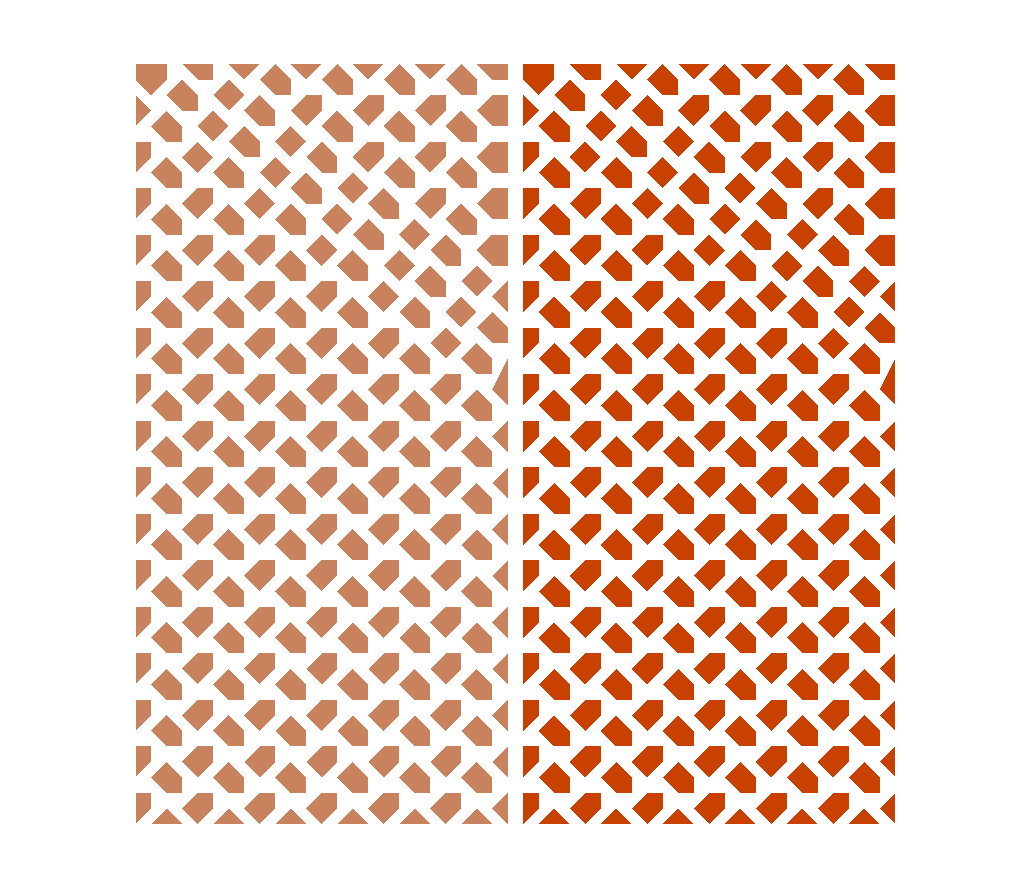
\includegraphics[width=0.3\textwidth]{pics/s4al1.png}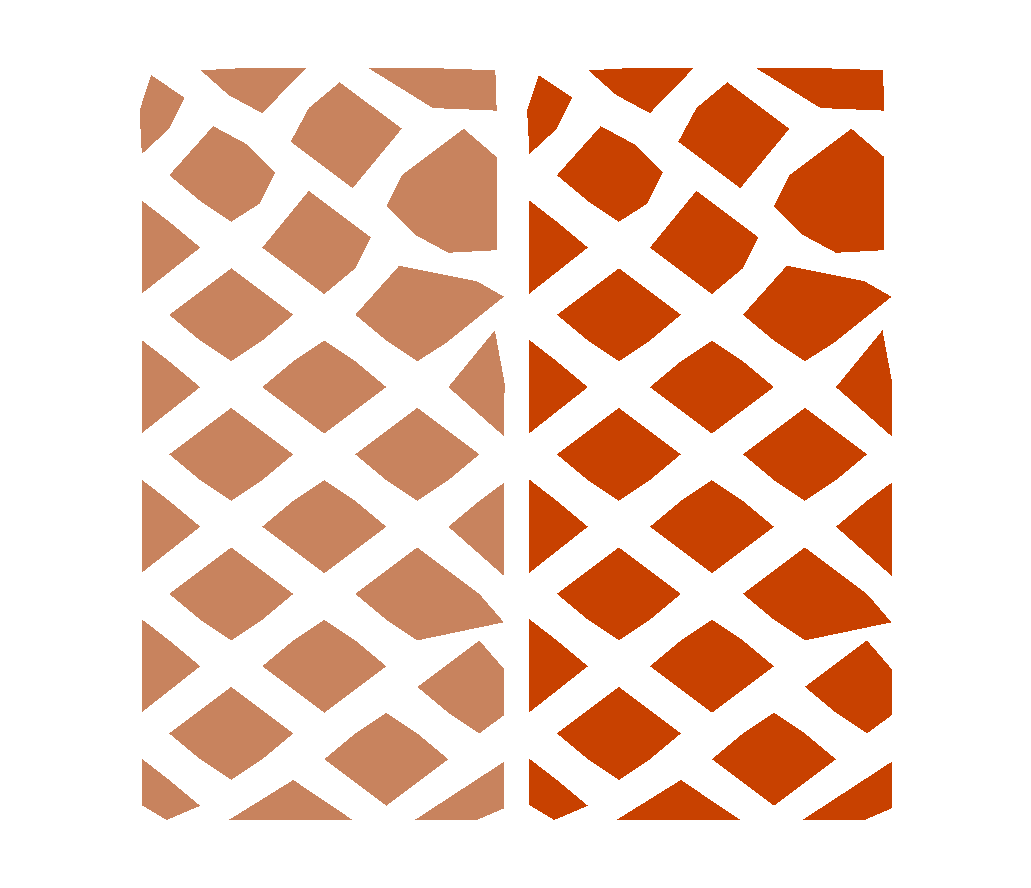
\includegraphics[width=0.3\textwidth]{pics/s4al2.png}
\includegraphics[width=0.3\textwidth]{pics/s4al3.png}}
\subfigure[Aggregates with settings from \texttt{xml/s4b.xml} (default parameters)]{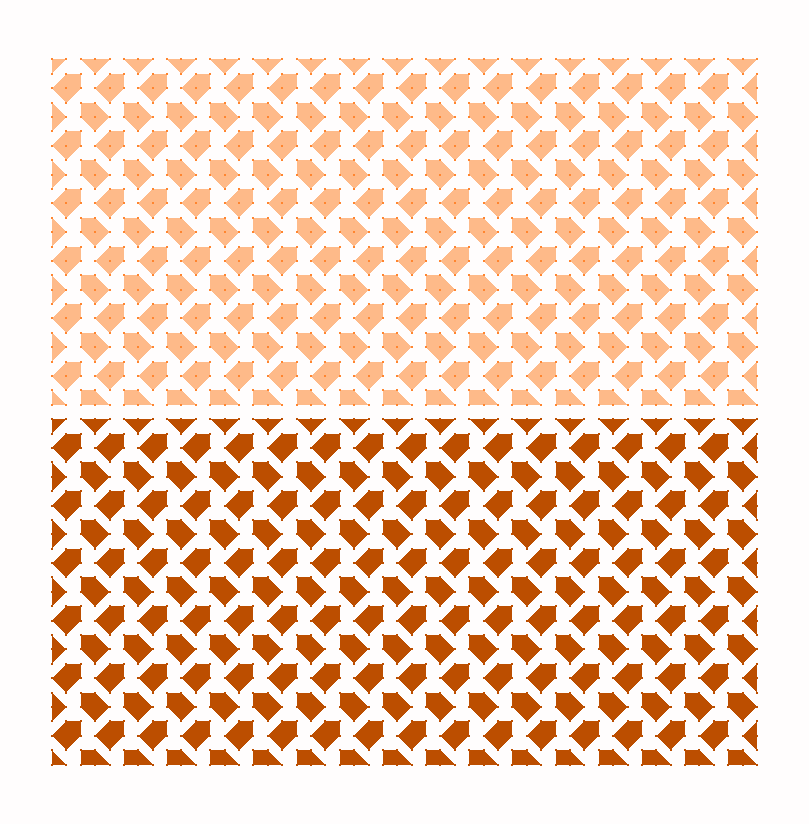
\includegraphics[width=0.3\textwidth]{pics/s4bl1.png}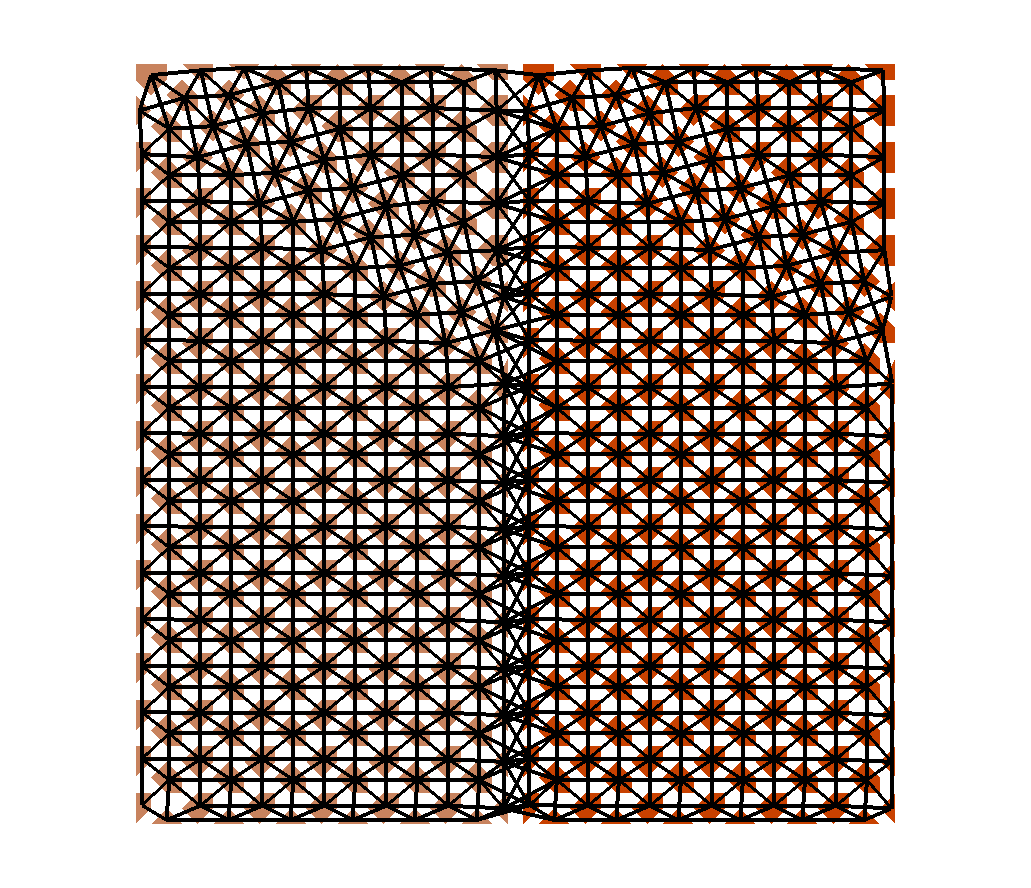
\includegraphics[width=0.3\textwidth]{pics/s4bl2.png}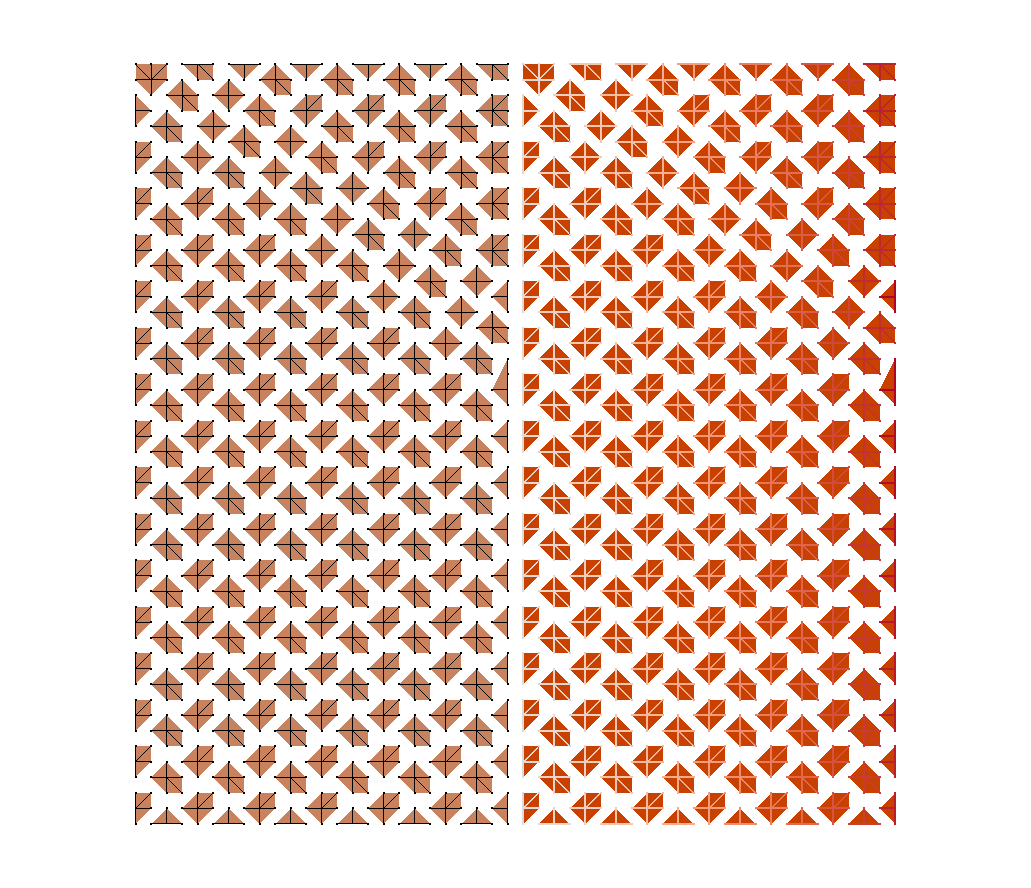
\includegraphics[width=0.3\textwidth]{pics/s4bl3.png}}
\caption{Different aggregation parameters and the corresponding aggregates}
\label{fig:diffaggregates}
\end{figure}

\chapter{Useful commands and debugging}

\section{Export level information}
Of course, it is possible to export the multigrid hierarchy in matrix market format similar to \S\ref{sec:exportdatasimple} when using the advanced XML file format instead of the simple XML format.

To export the multigrid hierarchy one can use, e.g., the following parameters

\lstinputlisting{../src/xml/s6_export.xml}

\section{Dependency trees}
\label{sec:dependencytrees}
For debugging it can be extremely helpful to automatically generate the dependency tree of the factories for a given XML file. However, it shall be noticed that even with a graphical dependency tree it might be hard to find the missing links and dependencies without a sufficient understanding of the overall framework.

To write out the dependencies you just have to put in the \verb|dependencyOutputLevel| parameter. The value gives you the fine level index that you are interested in (e.g., 1 means: print dependencies between level 1 and level 2).

\lstinputlisting{../src/xml/s6_dep.xml}

After running the example you should find a file named \verb|dep_graph.dot| in the current folder which you can transform into a graph using the \verb|dot| utility from the graphviz package.
Run, e.g. the following commands in your terminal to obtain the following graph:
\begin{verbatim}
sed -i 's/label=Graph\]/label=\"Graph\"\]/' dep_graph.dot
sed -i 's/\\"/"/g' dep_graph.dot
sed -i 's/"</</' dep_graph.dot
sed -i 's/>"/>/' dep_graph.dot
dot -Tpng dep_graph.dot -o dep_graph.dot.png
\end{verbatim}
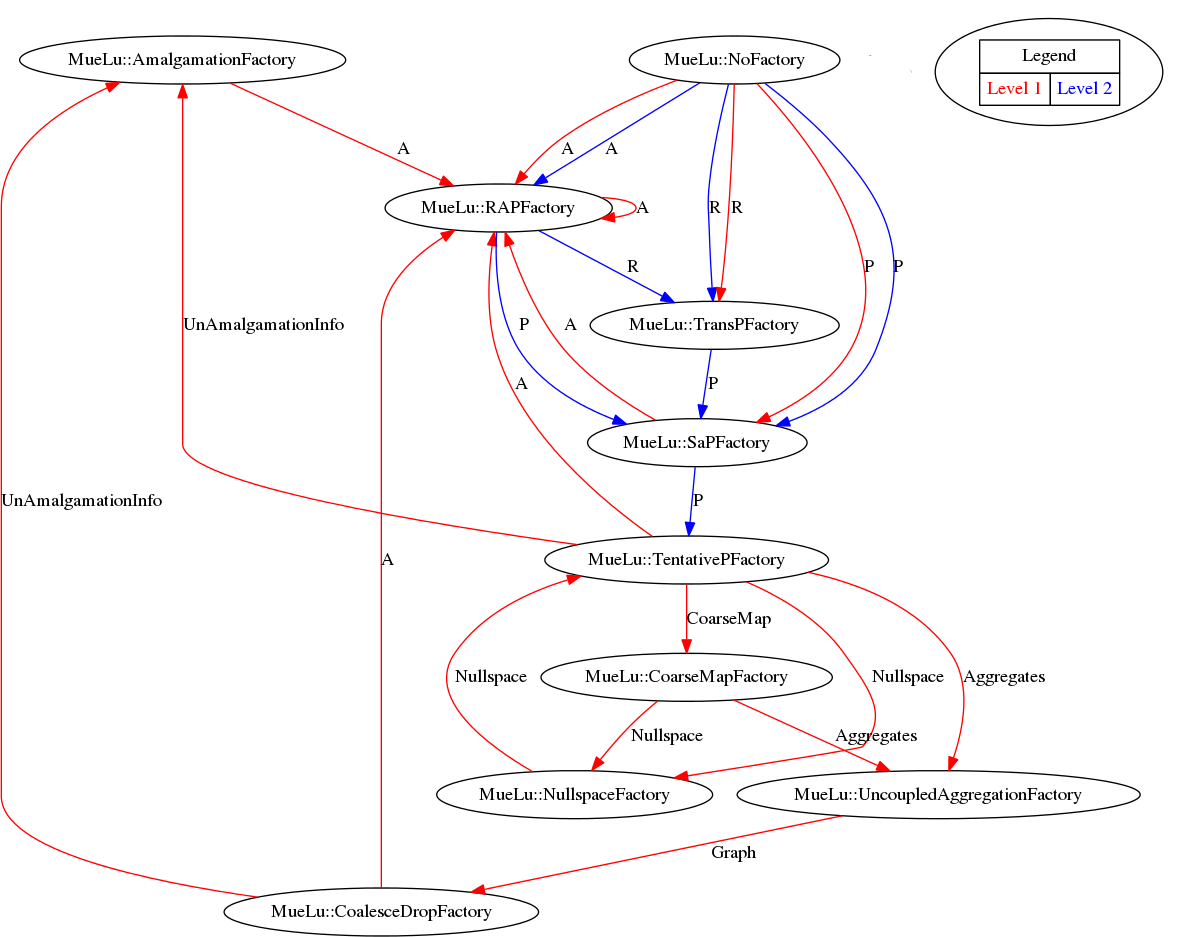
\includegraphics[width=1.0\textwidth]{pics/dep_graph} 

Note that the red arrows correspond to the fine level (level 1) and the blue arrows correspond to data on the coarse level (level 2).
Compare the factory layout in Figure \ref{fig:simpledesignaggregates} with above dependency graph. Try to read it from bottom to top.

\begin{mycomment}
In case that the file \verb|dep_graph.dot| is not generated you have to check the prerequisites. To be able to auto-generate the dependency graphs you have to compile \muelu with Boost enabled. Furthermore you have to set the \verb|MueLu_ENABLE_Boost_for_real:BOOL = ON| defines flag in your configuration script. If these requirements are not fulfilled you should find the error message \textit{Dependency graph output requires boost and MueLu\_ENABLE\_Boost\_for\_real} in the screen output of \muelu.
\end{mycomment}

As one can see from the dependency output there are also some internal factories which have not been visualized in the Figures \ref{fig:simpledesign}. A good example is the \verb|NullspaceFactory| which seems to build a dependency cycle with the \verb|TentativePFactory|. In fact, the \verb|NullspaceFactory| is a helper factory which allows to use the user-provided near null space vectors as input on the finest level. On the coarser levels it just loops through the generated coarse set of near null space vectors from the \verb|TentativePFactory|. This is a technical detail which sometimes can cause some problems when the corresponding dependency is not defined properly in the XML file.


\section{Graphical assistant for XML file generation}

The \verb|hands-on.py| driver script contains a graphical assistant to generate new XML parameter files in the advanced \muelu file format.

Just run the \verb|hands-on.py| script and choose a problem type from the list. Then choose option 2 to set the xml file. If you enter a filename that does not exist then the assistant is started to generate that new XML file.

\begin{center}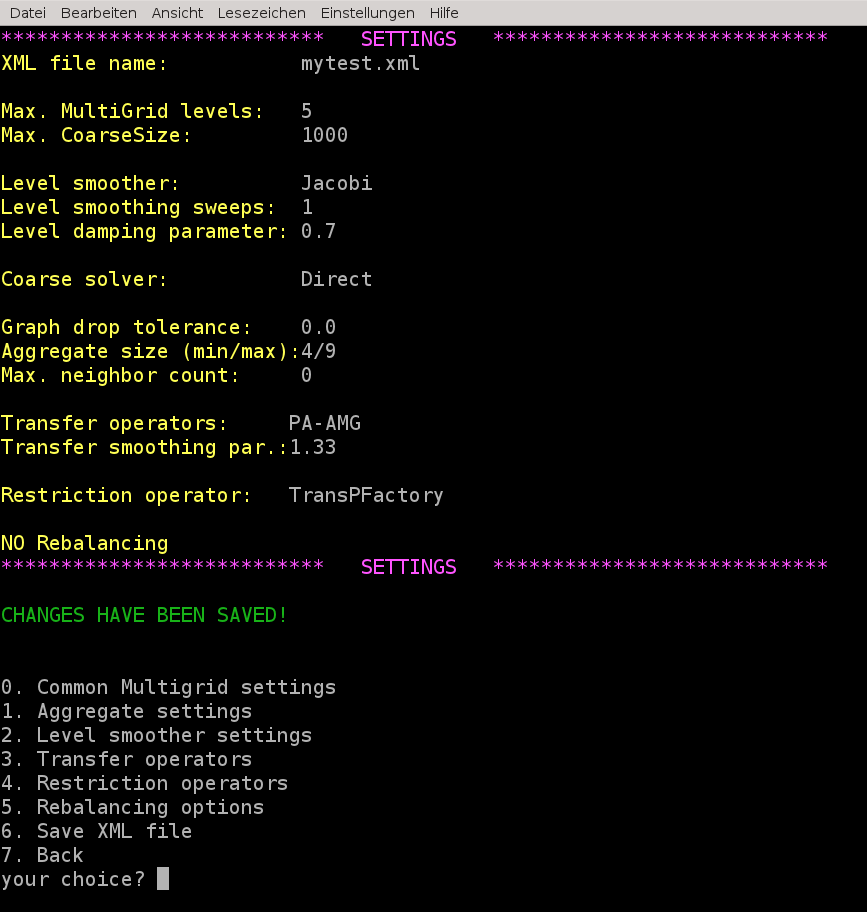
\includegraphics[width=10cm]{pics/tut1_15.png} \end{center}

Just go through the menu and make your choices for level smoothers, transfer operators and so on. Do not forget to call option 6 to save the XML file under the given name, that you have entered before. Then you can use option 7 to go back to the main menu for the example problem and try your new preconditioner with your parameter choices.

\begin{mycomment}
Of course, we could have introduced this feature with the earlier tutorials, but the idea was to familiarize the user with the XML files.
\end{mycomment}

\chapter{Challenge: elasticity example}
\section{Practical example}

For the second challenge, we consider an 2D elasticity example with $7020$ degrees of freedom. No further information is provided (geometry, discretization technique, \ldots).

\section{User-interface}
Run the \verb|hands-on.sh| script and choose the option 5 for the elasticity. The script automatically generates a XML file with reference multigrid parameters which are far from being optimal. The resulting problem matrix is symmetric. Therefore, we can use a CG method as outer linear solver.

\begin{exercise}
Open the \verb|stru2d_parameters.xml| file by pressing option 3. Try to find optimized multigrid settings using your knowledge from the previous tutorials. We have 2 (displacement) degrees of freedom per node and 3 vectors describing the near null space components (rigid body modes). All this information is automatically set correctly by the \verb|hands-on.py| script.
Run the example. Check the screen output (using option 1) and verify \verb|blockdim=2| on level 1 and \verb|blockdim=3| on level 2.
\end{exercise}

In the screen output of the \verb|CoalesceDropFactory| the \verb|blockdim| denotes the number of degrees of freedom per node (or super node on the coarser levels). Since the number of near null space vectors differs from the number of PDE equations, the number of degrees of freedom per node changes on the different multigrid levels.

\begin{exercise}
Open the XML parameter file (choose option 3) and try to find optimized settings. Use the advanced XML file format. Save the file, rerun the example (option 0) and compare the output with the reference results.
\end{exercise}

\begin{mycomment}
Use \S\ref{sec:generalhings} for a general step-by-step procedure to optimize the multigrid parameters.
\end{mycomment}

\begin{exercise}
How do the reference settings and your XML parameter settings perform when increasing the number of processors?
\end{exercise}

\begin{exercise}
Compare the results of the reference method and your preconditioner parameters when changing to a GMRES solver (instead of CG). What is changing? What about the solver timings?
\end{exercise}


\part{Expert tutorials}

\chapter{Using \muelu in user applications}

This tutorial demonstrates how to use \muelu from within user applications in C++. In \cite[Section 2.6]{Mue} it is explained how to use \muelu through the \texttt{MueLu::CreateE/TpetraPreconditioner} interface. This interface is designed for beginners which want to try \muelu through standard \trilinos interfaces. Note that there is also support for \stratimikos. Please refer to the \texttt{examples} in the \muelu folder for more details.

This tutorial aims at more advanced methods to use \muelu, creating an explicit instance of some \muelu classes like \texttt{MueLu::Hierarchy} and \texttt{MueLu::HierarchyManager}. In the next sections we give some code snippets. Most of them are borrowed form the \texttt{laplace2d.cpp} file in the tutorial.

\section{Preparations}
First of all, we have to define a communicator object. 
\printCppListing{laplace2d.cpp_2.fragment}

For the multigrid method we need a linear operator $A$. For demonstration purposes, here we just generate a 2D Laplacian operator using the \textsc{Galeri} package (see \ref{lab:examplesym}). In this example we use \epetra for the underlying linear algebra framework, but it shall be mentioned that it works for \tpetra in a similar way (refer to the code examples in the \muelu examples folder).
\printCppListing{laplace2d.cpp_4.fragment}

\muelu is based on \xpetra which provides a common interface both for \epetra and \tpetra. Therefore we have to encapsulate our \epetra objects into \xpetra wrapper objects. This is done using the following code.
\printCppListing{laplace2d.cpp_6.fragment}
Note that the \muelu setup routines require a \texttt{Xpetra::Matrix} object. The wrapper class \texttt{Xpetra::CrsMatrixWrap} is just a wrapper derived from \texttt{Xpetra::Matrix} which manages a \texttt{Xpetra::CrsMatrix} object which is the common base class for both \epetra and \tpetra CRS matrix classes. The details are not really important as long as one understands that one needs a \texttt{Xpetra::Matrix} object for \muelu in the end.
With the \texttt{SetFixedBlockSize} routine we state that there is only one degree of freedom per node (pure Laplace problem).
For aggregation-based algebraic multigrid methods one has to provide a valid set of near null space vectors to produce transfer operators. In case of a Laplace problem we just use a constant vector.
\printCppListing{laplace2d.cpp_8.fragment}

\section{Setup phase}

With a fine level operator $A$ available as \texttt{Xpetra::Matrix} object and a set of near null space vectors (available as \texttt{Xpetra::MultiVector}) all minimum requirements are fulfilled for generating an algebraic multigrid hierarchy. There are two different ways to setup a multigrid hierarchy in \muelu. One can either use a parameter list driven setup process which accepts either \texttt{Teuchos::ParameterList} objects or XML files in two different XML file formats. Alternatively, one can use the \muelu C++ API to define the multigrid setup at compile time. In the next sections we show both variants.

\subsection{XML Interface}

The most comfortable way to declare the multigrid parameters for \muelu is using the XML interface. In fact, \muelu provides two different XML interfaces. There is a simplified XML interface for multigrid users and a more advanced XML interface for expert which allows to make use of all features of \muelu as a multigrid framework. Both XML file formats are introduced in the previous sections of this hands on tutorial. 
However, for the C++ code it makes no difference which type of XML interface is used.

Assuming that we have a \texttt{Teuchos::ParameterList} object with valid \muelu parameters we can create a \texttt{MueLu::HierarchyManager} object
%First of all, one has to create a \texttt{MueLu::ParameterListInterpreter} object which either accepts a \texttt{Teuchos::ParameterList} or a file with XML parameters.
\printCppListing{ScalingTestParamList.cpp_2.fragment}
For an example how to fill the parameter list the reader may refer to \cite[Section 2.3]{Mue}. Note that there are routines to fill the parameter lists with the information from XML files. You can also directly provide a file name of a XML file to the \texttt{Muelu::ParameterListInterpreter}. For details you may refer to the doxygen documentation or the example in \texttt{laplace2d.cpp}.

Next a new \texttt{MueLu::Hierarchy} object is generated
\printCppListing{ScalingTestParamList.cpp_4.fragment}
The \texttt{CreateHierarchy} creates a new empty multigrid hierarchy with a finest level only. The user has to feed in the linear operator $A$ and the near null space vector. If further information is available, such as the node coordinates, they can be also stored in the finest level. The coordinates are needed, e.g., for rebalancing the coarse levels.
Finally, the \texttt{SetupHierarchy} call initiates the coarsening process and the multigrid hierarchy is built according to the parameters from the \texttt{mueluList} parameters. 
\printCppListing{ScalingTestParamList.cpp_6.fragment}

As XML parameter file any of the files shown in the previous tutorials can be used.

\begin{mycomment}
As one can see from the last code snippet, the \texttt{Hierarchy} allows access to all important parts of the multigrid method before setup. So, if you have to feed in some non-standard information, this is the way how it works. Using the \texttt{CreateE/TpetraPreconditioner} interface may be easier but does not allow to access the finest level before setup. 
\end{mycomment}

Once the \texttt{SetupHierarchy} call is completed, the multigrid hierarchy is ready to use. The reader can skip the next section about the C++ interface and proceed with \S\ref{sec:muelu_belospreconditioner} for an example how to use the multigrid method as preconditioner within a Krylov subspace method from the \belos package.

\subsection{C++ Interface}

As an alternative to the XML interfaces, the user can also define the multigrid hierarchy using the C++ API directly. In contrary to the XML interface which allows to build the layout of the multigrid preconditioner at runtime, the preconditioner is fully defined at compile time when using the C++ interface.

First, a \texttt{MueLu::Hierarchy} object has to be defined, which manages the multigrid hierarchy including all multigrid levels. It provides routines for the multigrid setup and the multigrid cycle algorithms (such as V-cycle and W-cycle).
\printCppListing{ScalingTest.cpp_6.fragment}

There are some member functions which can be used to describe the basic multigrid hierarchy. The \texttt{SetMaxCoarseSize} member function is used to set the maximum size of the coarse level problem before the coarsening process can be stopped.
\printCppListing{ScalingTest.cpp_8.fragment}

Next, one defines an empty \texttt{MueLu::Level} object for the finest level. The \texttt{MueLu::Level} objects represent a data container storing the internal variables on each multigrid level. The user has to provide and fill the level container for the finest level only. The \texttt{MueLu::Hierarchy} object then automatically generates the coarse levels using the multigrid parameters. The absolute minimum requirements for the finest level that the user has to provide is the fine level operator $A$ which represents the fine level matrix. \muelu is based on \xpetra. So, the matrix $A$ has to be of type \texttt{Xpetra::Matrix}. In addition, the user should also provide a valid set of near null space vectors. For a Laplace problem we can just use the constant \texttt{nullspace} vector that has previously been defined. Some routines need additional information. For example, the user has to provide the node coordinates for repartitioning.
\printCppListing{ScalingTest.cpp_10.fragment}
\begin{mycomment}
When including the \texttt{MueLu\_UseShortNames.hpp} header file the template parameters usually can be dropped for compiling. The most important template parameters are \texttt{SC} for the scalar type, \texttt{LO} for the local ordinal type (usually \texttt{int}) and \texttt{GO} for the global ordinal type. For a detailed description of the template parameters the reader may refer to the \tpetra documentation.
\end{mycomment}

A \texttt{MueLu::FactoryManager} object is used for the internal management of data dependencies and generating algorithms of the multigrid setup. Even though not absolutely necessary, we show the usage of the \texttt{MueLu::FactoryManager} object as it allows for  user-specific enhancements of the multigrid code.
\printCppListing{ScalingTest.cpp_12.fragment}

The user can define its own factories for performing different tasks in the setup process. The following code shows how to define a smoothed aggregation transfer operator and a restriction operator. The \texttt{MueLu::RAPFactory} is used for the (standard) Galerkin product to generate the coarse level matrix $A$.
\printCppListing{ScalingTest.cpp_14.fragment}

The user-defined factories have to be registered in the \texttt{FactoryManager} using the lines
\printCppListing{ScalingTest.cpp_16.fragment}
\begin{mycomment}
If you forget to register the new factories, the \texttt{FactoryManager} will use some internal default factories for being responsible to create the corresponding variables. Then your user-specified factories are just ignored during the multigrid setup!
\end{mycomment}
Note, that the \texttt{FactoryManager} is also responsible for resolving all dependencies between different factories. That is, after the user-defined factories have been registered, all factories that request variable $P$ are provided with the prolongation operator $P$ that has been generated by the registered factory \texttt{PFact}. If there is some data requested for which no factory has been registered by the user, the \texttt{FactoryManager} manages an internal list for reasonable default choices and default factories.

Next, the user has to declare a level smoother. The following code can be used to define a symmetric Gauss-Seidel smoother. Other methods can be set up in a similar way.
\printCppListing{ScalingTest.cpp_18.fragment}
Before the level smoother can be used, a \texttt{MueLu::SmootherFactory} has to be defined for the smoother factory. The \texttt{SmootherFactory} is used in the multigrid setup to generate level smoothers for the corresponding levels using the prototyping design pattern. Note, that the \texttt{SmootherFactory} has also to be registered in the \texttt{FactoryManager} object. If the user forgets this, the multigrid setup will use some kind of default smoother, i.e., the user-chosen smoother options are just ignored.
\printCppListing{ScalingTest.cpp_20.fragment}
Once the \texttt{FactoryManager} is set up, it can be used with the \texttt{Hierarchy::Setup} routine to initiate the coarsening process and set up the multigrid hierarchy.
\printCppListing{ScalingTest.cpp_22.fragment}

\section{Iteration phase}
\label{sec:iterationphase}
Once the setup phase is completed, the \muelu multigrid hierarchy is ready for being used.

There are several ways how to use the multigrid method. One can apply the multigrid method as standalone solver for linear systems. Multigrid methods are also known to be efficient preconditioners within iterative (Krylov) solvers such as CG or GMRES methods.

In the next subsections it is demonstrated how to use \muelu as standalone solver and as preconditioner for iterative solvers from the \belos and \aztecoo package in \trilinos.

For solving a linear system $Ax=b$ we need a right hand side vector $b$. When using iterative solvers we also need an initial guess for the solution vector. 
\printCppListing{laplace2d.cpp_7.fragment}
In this example we just create \epetra vectors and wrap them into \xpetra objects. The right hand side vector is initialized with one and the solution vector is filled with random values.

\subsection{\muelu as multigrid solver}
To use \muelu as standalone solver one can use the following code
\printCppListing{laplace2d.cpp_18.fragment}
In this code snippet a solution vector is created using the \texttt{Xpetra::VectorFactory} and initialized with the content from the solution vector \verb|xX| containing the initial guess. Then, the \texttt{MueLu::Hierarchy} object is set to the non-preconditioner mode and the \texttt{Iterate} routine is called
to perform \texttt{mgridSweeps} sweeps with the chosen multigrid cycle. If successful, the \texttt{mgridLsgVec} vector contains the solution.

\subsection{\muelu as preconditioner for \aztecoo}
Commonly, multigrid methods are used as preconditioners for iterative linear solvers. Here, we show how to use the \texttt{MueLu::Hierarchy} as preconditioner within an \aztecoo solver (using \epetra).
After an \epetra solution vector has been created by 
\lstinputlisting[firstline=2]{laplace2d.cpp_14.fragment}
the following code can be used to apply the \muelu hierarchy as preconditioner within the \aztecoo CG solver
\lstinputlisting[firstline=2]{laplace2d.cpp_16.fragment}
Basically, the \muelu hierarchy is put into an \texttt{MueLu::EpetraOperator} object, which implements the \epetra interface for preconditioners.
With the \texttt{SetPrecOperator} routine from the \aztecoo solver the \texttt{MueLu::EpetraOperator} object then is defined as preconditioner.

\subsection{\muelu as preconditioner for \belos}
\label{sec:muelu_belospreconditioner}
%% common part

\belos is the successor package of \aztecoo for linear solvers in \trilinos and works both for \epetra and \tpetra. Here we demonstrate how to use \muelu as preconditioner for \belos solvers using \xpetra.
First, we have to declare objects for the solution vector and the right hand side vector in \xpetra. The following code just uses a random vector for the initial guess and solution variable.
\printCppListing{ScalingTest.cpp_24.fragment}

In the following we demonstrate how to use the \muelu hierarchy as preconditioner within a \belos solver. There are special wrapper objects for wrapping the \xpetra matrix and the \muelu hierarchy to \belos compatible objects. These can be used to define a linear problem for use with \belos.
\printCppListing{ScalingTest.cpp_26.fragment}

Then, one can set up the \belos solver. For a \belos GMRES solver one uses
\printCppListing{ScalingTest.cpp_28.fragment}
Finally, we can solve the linear system using \belos with the \muelu multigrid preconditioner (left-preconditioning) by calling
\printCppListing{ScalingTest.cpp_30.fragment}
and perform some convergence checks
\printCppListing{ScalingTest.cpp_32.fragment}

\section{Full example}

The reader may refer to \texttt{laplace2d.cpp} for a working example to study the source code. This demonstration program has some more features that are not discussed in this tutorial.

\begin{exercise}
Compile the example in \texttt{laplace2d.cpp} and then run the program in parallel using two processors
        \begin{verbatim}
        mpirun -np 2 ./MueLu_tutorial_laplace2d.exe --help
        \end{verbatim}
        Study the screen output and try to run the example with an XML file as input for the multigrid setup.
\end{exercise}
\begin{exercise}
Create large scale examples using the \verb|nx| and \verb|ny| parameters for a finer mesh. Choose reasonable numbers for \verb|nx| and \verb|ny| for your machine and make use of your knowledge about \muelu for generating efficient preconditioners.
\end{exercise}

\chapter{ML ParameterList interpreter}

\section{Backwards compatibility}
\ml \cite{mlguide} is the predecessor multigrid package of \muelu in \trilinos and widely used in the community for smoothed aggregation multigrid methods. \ml is implemented in C and known for its good performance properties. However, the disadvantage is that \ml is harder to adapt to new applications and non-standard problems. Furthermore, \ml uses its own internal data structure and is somewhat limited to the use with \epetra objects only. In contrast, \muelu provides a fully flexible multigrid framework which is designed to be adapted to any kind of new application with non-standard requirements. Furthermore, it is based on \xpetra and therefore can be used both with \epetra or \tpetra. Nevertheless, it is an important point to provide some kind of backwards compatibility to allow \ml users to easily migrate to \muelu (or make experiments with \muelu without having to write to much new code).

In this tutorial we present the \texttt{MueLu::MLParameterListInterpreter} which provides support for the most important \ml parameters to be used with \muelu.

\section{C++ part}

\subsection{Preparations}
In order to use \muelu (instead or aside of \ml) you first have to add it to your application. Please refer to the \muelu user guide for information about compilation and linking (see \cite{Mue}). Basically, if your application is already working with \ml you should only need to compile and install \muelu and make sure that the \muelu libraries are found by the linker.

\subsection{C++ interface}


In the following we assume that the linear operator $A$ is available as \verb|RCP<Xpetra::Matrix> A|.

Then we create a parameter list and fill it with \ml parameters. Please refer to the \ml guide \cite{mlguide} for a complete list of available parameters.
\printCppListingSkipLine{MLParameterList.cpp_6.fragment}

\begin{mycomment}
Be aware that the \verb|MLParameterListInterpreter| does not support all \ml parameters but only the most important ones (e.g., smoothers, transfer operators, rebalancing, ...). There is, e.g., no support for the Maxwell specific enhancements in \ml.
\end{mycomment}

Instead of defining the \ml parameters by hand in the ParameterList you can also read in XML files with \ml parameters using
\printCppListingSkipLine{MLParameterList.cpp_4.fragment}

Next, you create a \verb|MLParameterListInterpreter| object using the parameters and create a new \verb|MueLu::Hierarchy| from it.
\printCppListingSkipLine{MLParameterList.cpp_8.fragment}

Of course, we have to provide all necessary information for the multigrid setup routine. This does not only include the fine level operator but also the set of near null space vectors. Assuming that \verb|numPDEs| stores the number of equations (and near null space vectors) the following code allows to produce piecewise constant standard near null space vectors (which should be valid for many PDE discretizations).
\printCppListingSkipLine{MLParameterList.cpp_10.fragment}

Then we just feed in the information to the finest level
\printCppListingSkipLine{MLParameterList.cpp_11.fragment}

Finally we call the \verb|Setup| routine which actually builds the multigrid hierarchy.
\printCppListingSkipLine{MLParameterList.cpp_13.fragment}

Once we have the multigrid hierarchy set up we can use it the same way as described in \S\ref{sec:iterationphase}.

\begin{exercise}
Study the source code of \texttt{../src/MLParameterList.cpp} and compile it. Run the executable \verb|MueLu_tutorial_MLParameterList.exe| with the \verb|--help| command line parameter to get an overview of all available command line parameters. Run the example using
\begin{verbatim}
./MueLu_tutorial_MLParameterList.exe --ml=1 --muelu=0 
   --xml=xml/ml_ParameterList.xml --linAlgebra=Epetra
\end{verbatim}
and study the \ml output. Compare the output and results when switching to \muelu using the same input file
\begin{verbatim}
./MueLu_tutorial_MLParameterList.exe --ml=0 --muelu=1 
   --xml=xml/ml_ParameterList.xml --linAlgebra=Epetra
\end{verbatim}
\end{exercise}

\begin{exercise}
Play around with the parameters from \verb|MueLu_tutorial_MLParameterList.exe|. Change, e.g., the problem type to a 2D Laplace problem (\verb|--matrixType=Laplace2D|) and adapt the \verb|--nx| and \verb|--ny| parameters accordingly.
Try to run both \ml and \muelu and compare the results. Do you find significant differences?
\end{exercise}

\appendix
\part{Appendix}

\chapter{Virtual box image}

This chapter discusses the basics of the virtual box image that comes with this tutorial to allow the user to follow above explanations and do its own experiments with \muelu and \trilinos. A virtual machine has the advantage that it is rather easy to set up for a user. Even though compiling and installing got easier the last years by using a cmake based build system it is still a nightmare for not so experienced users. The virtual machine runs both on Linux and Windows as host and brings all the necessary tools for a quick start to \muelu.

\section{Preparations}

To use the virtual machine you basically have to perform the following steps.

\begin{enumerate}
\item Install \verb|VirtualBox| on your host machine. You can download it from \verb|www.virtualbox.org|.
\item Download the \verb|MueLu_Tutorial.ova| virtual machine. The image file has 4 GB.
\item Run \verb|VirtualBox| and import the \verb|MueLu_Tutorial.ova| machine.
\begin{center}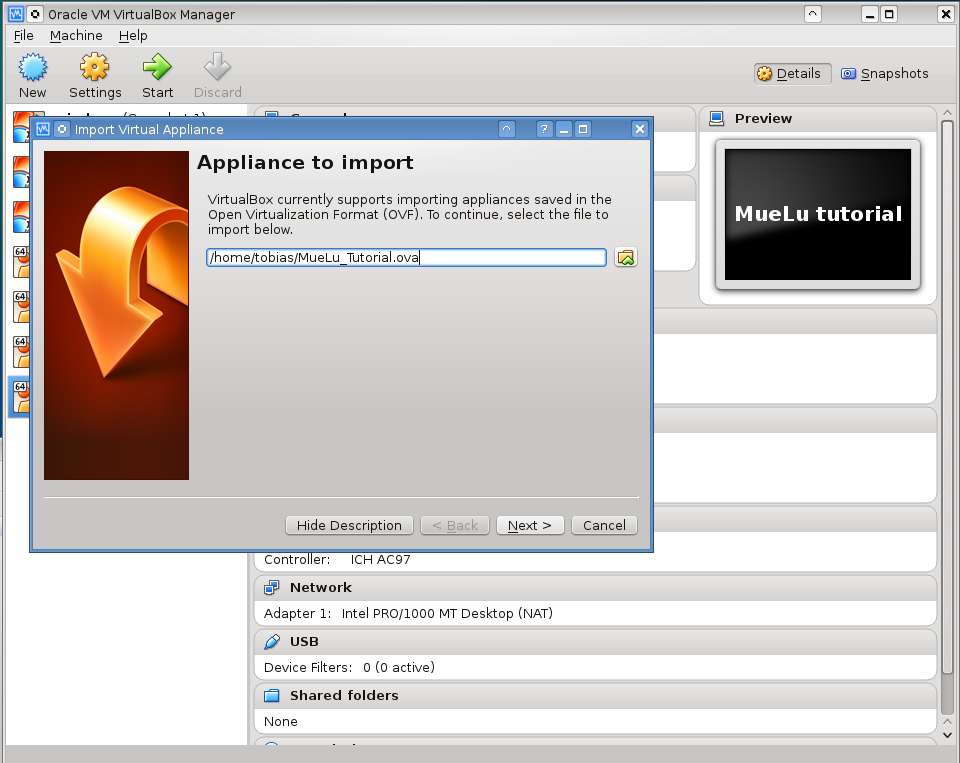
\includegraphics[width=0.8\textwidth]{pics/installation_1.png} \end{center}
Then, check and adapt the settings of the virtual machine. 
\begin{center}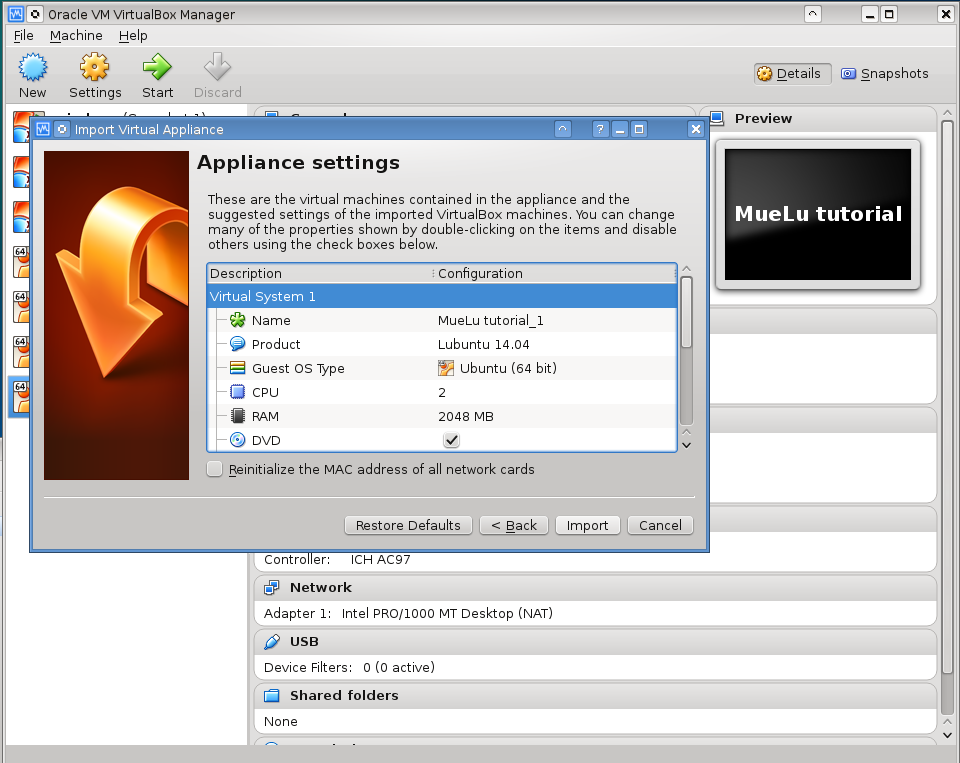
\includegraphics[width=0.8\textwidth]{pics/installation_2.png} \end{center}
In general, one processor should be enough. But if you want to make some more reasonable tests with parallel multigrid you should increase the number of processors accordingly. 
Click import, to import the virtual machine.
\item With a click on the start button the virtual machine is booting.
\end{enumerate}

\section{First steps}

\subsection{Login and setup}

Once the virtual machine is started you first have to login. 

\begin{center}\includegraphics[width=0.8\textwidth]{pics/lubuntu_1.png} \end{center}

The login data is:
\begin{center}
\begin{tabular}{ll}
Username: & muelu \\
Password: & sandia
\end{tabular}
\end{center}

\begin{mycomment}
You only need to enter the password in above screen.
\end{mycomment}

After the login you should see the following desktop.
\begin{center}\includegraphics[width=0.8\textwidth]{pics/lubuntu_2.png} \end{center}

First, you should adapt the language settings and the keyboard layout. You can switch the keyboard layout by clicking on the logo in the lower right corner. A right click on the logo allows you to change more details
\begin{center}\includegraphics[width=0.8\textwidth]{pics/lubuntu_3.png} \end{center}

Then you are ready to go with the tutorial.

\subsection{\muelu tutorial}

Open the tutorial with \verb|evince| as pdf viewer. To open \verb|evince| you can either use the shortcut in the lower left corner of your desktop or press \Alt+\keystroke{F2} to open the \verb|Run| dialog and enter \verb|evince|. Load the \verb|muelu_tutorial.pdf| file in the \verb|tutorial| folder of your home directory.

To open a terminal you have several option. Either use the shortcut button in the lower left corner. Alternatively you can open the \verb|Run| dialog (\Alt+\keystroke{F2}) and enter \verb|lxterminal|. As a third alternative you can just press \Ctrl+\Alt+\keystroke{T}. In the terminal, change to the \verb|tutorial| folder by entering \verb|cd tutorial|. Therein you can find the \verb|hands-on.py| script which is used throughout the whole \muelu tutorial.

\begin{center}\includegraphics[width=0.8\textwidth]{pics/lubuntu_4.png} \end{center}

\begin{mycomment}
Use the \keystroke{Win}+\LArrow and \keystroke{Win}+\RArrow keys to arrange the windows in a split view as shown above.
There are other useful keyboard shortcuts such as \keystroke{Win}+\keystroke{R} to open the \verb|Run| dialog or \keystroke{Win}+\keystroke{E} to open the file manager.
\end{mycomment}

When plotting the results with gnuplot from within the \verb|hands-on.py| script it might be useful to make the plot windows to stay on top.

\begin{center}\includegraphics[width=0.8\textwidth]{pics/lubuntu_5.png} \end{center}

The virtual machine has all software installed that you need to follow the tutorial (including \verb|paraview|)

\begin{center}\includegraphics[width=0.8\textwidth]{pics/lubuntu_6.png} \end{center}

\section{Software}

The virtual machine is based on a minimal installation of \textbf{Lubuntu 14.04}. The image file has 4 GB with about 250 MB free for the user. 

The following software is pre-installed:

\begin{tabular}{ll}
Web-browser: & midori \\
PDF-viewer:  & evince \\
Terminal:    & LXTerminal\\
Visualization: & paraview, gnuplot \\
File manager: & PCManFM \\
\end{tabular}

The following system libraries are installed:

\begin{tabular}{ll}
Trilinos:     & Trilinos (developer branch: Oct 1, 2014) \\
Direct solver: & SuperLU 4.3 \\
VTK: & VTK 5.8 \\
MPI: & OpenMPI 1.6.5 \\
Python: & Python 2.7.6 \\
Compiler: & gcc 4.8.2
\end{tabular}

\lstset{%
    float=hbp,%
    basicstyle=\ttfamily\small, %
    identifierstyle=\color{colIdentifier}, %
    keywordstyle=\color{colKeys}, %
    stringstyle=\color{colString}, %
    commentstyle=\color{colComments}, %
    columns=flexible, %
    tabsize=2, %
    frame=none, %
    extendedchars=true, %
    showspaces=false, %
    showstringspaces=false, %
    numbers=none, %
    breaklines=true, %
    backgroundcolor=, %
    breakautoindent=true, %
    captionpos=b%
}

\chapter{Error messages}

\section{Syntax errors}

\subsection{Parser errors}
\begin{cBox}
\begin{lstlisting}
XML parse error at line 27: file ended before closing element 'ParameterList' from line 1
\end{lstlisting}
\end{cBox}
Forgot to close the \verb|</ParameterList>| section that is opened in line 1 of the xml file.

\begin{cBox}
\begin{lstlisting}
XML parse error at line 15: start element not well-formed: invalid character
\end{lstlisting}
\end{cBox}
Check line 15 for an invalid xml format. The reason can be, e.g., a missing closing character \verb|/>| for a parameter.

\subsection{Parameter list errors}
\begin{cBox}
\begin{lstlisting}
All child nodes of a ParameterList must have a name attribute!
\end{lstlisting}
\end{cBox}
You probably forgot to add a name attribute in one or more elements of your xml file, that is you used, e.g., 
\begin{lstlisting}
<Parameter  type="string" value="RELAXATION"/>
\end{lstlisting}
instead of
\begin{lstlisting}
<Parameter name="smoother: type" type="string" value="RELAXATION"/>
\end{lstlisting}



\begin{cBox}
\begin{lstlisting}
Error, the parameter {name="smoother: type",type="int",value="0"}
in the parameter (sub)list "ANONYMOUS"
exists in the list of valid parameters but has the wrong type.

The correct type is "string".
\end{lstlisting}
\end{cBox}
Use the correct (proposed) value type for the given parameter name, i.e., 
\begin{lstlisting}
<Parameter name="smoother: type" type="string" value="RELAXATION"/>
\end{lstlisting} 
instead of
\begin{lstlisting}
<Parameter name="smoother: type" type="int" value="RELAXATION"/>
\end{lstlisting}

\section{\muelu errors}

\subsection{General errors}

\begin{cBox}
\begin{lstlisting}
Throw test that evaluated to true: s_.is_null()

Smoother for Epetra was not constructed
    during request for data "    PreSmoother" on level 0 by factory NoFactory
\end{lstlisting}
\end{cBox}
Failed to create a level smoother. Check the smoother blocks in your xml file.
The error occurs, e.g., if there is a typing error in the \verb|smoother: type| parameter.
For example
\begin{lstlisting}
<Parameter name="smoother: type" type="string" value="REXATION"/>
\end{lstlisting}
would trigger above error since the smoother type should be \verb|RELAXATION|.

\begin{cBox}
\begin{lstlisting}
IFPACK ERROR -2, ifpack/src/Ifpack_PointRelaxation.cpp, line 117
\end{lstlisting}
\end{cBox}
Errors like this indicate that it is a problem within the \verb|smoother: params| section. Most likely a (relaxation) smoother is requested which is not existing (e.g., \verb|Jadobi| instead of \verb|Jacobi|).

\begin{cBox}
\begin{lstlisting}
The parameter name "smother: type" is not valid. Did you mean "smoother: type"?
\end{lstlisting}
\end{cBox}
There is a typo in your parameter list. Locate the parameter and fix it (using the suggestions, that come with the error message).

\begin{cBox}
\begin{lstlisting}
Throw test that evaluated to true: maxNodesPerAggregate < minNodesPerAggregate
\end{lstlisting}
\end{cBox}
Choose the \verb|aggregation: min agg size| parameter to be smallter than the \verb|aggregation: max agg size| parameter for the aggregation routine.

\subsection{Advanced XML file format}

\begin{cBox}
\begin{lstlisting}
Throw test that evaluated to true: bIsZeroNSColumn == true

MueLu::TentativePFactory::MakeTentative: fine level NS part has a zero column
\end{lstlisting}
\end{cBox}
This error indicates that there is a problem with the provided near null space vectors. There are different reasons which can trigger this problem:
\begin{itemize}
\item The near null space vectors are not valid (containing zeros, wrong ordering of internal degrees of freedom). Please check your near null space vectors. Maybe there is an empty vector or the ordering of degrees of freedom for the linear operator does not match with the ordering of the near null space vectors.
\item The near null space vectors are correct but used in a wrong way (e.g., a wrong number of degrees of freedom). Check the screen output for wrong block dimensions (CoalesceDropFactory).
\item There is a problem with the aggregates. Validate the screen output and look for unusual (e.g. very small or empty) aggregates.
\end{itemize}


\begin{cBox}
\begin{lstlisting}
Throw test that evaluated to true: factoryManager_ == null

MueLu::Level(0)::GetFactory(Aggregates, 0): No FactoryManager
\end{lstlisting}
\end{cBox}
This is a typical error when the dependency tree is screwed up. If aggregates and/or transfer operators are involved usually one has forgotten some entries in the \verb|Hierarchy| sublist of the extended XML file format for the internal factory managers. These errors can be quite tricky to fix. In general it is a good idea to start with a working XML file and extend it step by step if possible.
The following general strategies may help to track down the problem:
\begin{itemize}
\item Run the problem with \verb|verbosity=high| to get as much screen output as possible. Check for unusual screen output (such as \verb|Nullspace factory|.
\item Try to generate a graphical dependency tree as described in \S\ref{sec:dependencytrees}.
\end{itemize}

For example, above error is caused by the following XML file

\lstset{%
    float=hbp,%
    basicstyle=\ttfamily\small, %
    identifierstyle=\color{colIdentifier}, %
    keywordstyle=\color{colKeys}, %
    stringstyle=\color{colString}, %
    commentstyle=\color{colComments}, %
    columns=flexible, %
    tabsize=2, %
    frame=single, %
    extendedchars=true, %
    showspaces=false, %
    showstringspaces=false, %
    numbers=left, %
    numberstyle=\tiny, %
    breaklines=true, %
    backgroundcolor=\color{ocre!20!white}, %
    breakautoindent=true, %
    captionpos=b%
}
\begin{lstlisting}
<ParameterList name="MueLu">
  <ParameterList name="Factories">   
    <ParameterList name="myTentativePFact">
      <Parameter name="factory"                             type="string" value="TentativePFactory"/>
    </ParameterList>
  </ParameterList>

  <ParameterList name="Hierarchy">
    <ParameterList name="Levels">
      <Parameter name="P"          type="string" value="myTentativePFact"/>
      <!--<Parameter name="Nullspace"          type="string" value="myTentativePFact"/>-->
    </ParameterList>
  </ParameterList>
</ParameterList>
\end{lstlisting}

\lstset{%
    float=hbp,%
    basicstyle=\ttfamily\small, %
    identifierstyle=\color{colIdentifier}, %
    keywordstyle=\color{colKeys}, %
    stringstyle=\color{colString}, %
    commentstyle=\color{colComments}, %
    columns=flexible, %
    tabsize=2, %
    frame=none, %
    extendedchars=true, %
    showspaces=false, %
    showstringspaces=false, %
    numbers=none, %
    breaklines=true, %
    backgroundcolor=, %
    breakautoindent=true, %
    captionpos=b%
}

Looking at the error output it seems to be a problem with aggregates. However, in the XML file no special aggregation factory has been declared. The only factory which has been introduced was a tentative prolongation factory for generating unsmoothed transfer operators. Therefore, one should start digging into the details of the \verb|TentativePFactory| to find out that the unsmoothed transfer operator factory is responsible both for creating the unsmoothed prolongator and the coarse level null space information. When looking at the screen output one should find that the last called/generated factory is a \verb|NullspaceFactory| which can also be a hint that the problem is the null space.

When looking at the XML file one can see that the \verb|myTentativePFact| factory has been registered to be responsible for generating  the prolongator $P$, but the generating factory for the variable \verb|Nullspace| is not declared. \muelu tries to generate the default null space, but since it does not know about \verb|myTentativePFact| to be a \verb|TentativePFactory| which would already produce the needed information the calling ordering of the dependent factories (e.g., aggregation) gets mixed up.

Note that the \verb|TentativePFactory| is special. If you declare an explicit instance of the \verb|TentativePFactory| you always have to register it for generating the \verb|Nullspace| variable, too. Only in very special cases this would not be necessary.

\begin{mycomment}
This is a general rule: if a factory generates more than one output variables, always make sure that all these output variables are properly defined in the \verb|FactoryManager| list (or \verb|Hierarchy| sublist in the xml files, respectively).
\end{mycomment}

To solve above problem there are two possibilities:
\begin{itemize}
\item Following above comment, just register \verb|myTentativePFact| for generating \verb|Nullspace|. That is, just comment in the corresponding line in above xml file.
\item Alternatively you can register \verb|myTentativePFact| for generating \verb|Ptent| (and \verb|P|). This way you mark the \verb|myTentativePFact| object to be used for generating the unsmoothed transfer operators (and state that they shall be used for the final prolongation operators). \muelu is smart enough to understand that the factory responsible for generating \verb|Ptent| is also supposed to generate the null space vectors.
\end{itemize}


\begin{thebibliography}{99}
\bibitem{briggs} W.L. Briggs, S.F. McCormick and others, A multigrid tutorial, SIAM, 2000.
\bibitem{Mue} A. Prokopenko, J.J. Hu, T.A. Wiesner, C.M. Siefert and R.S. Tuminaro \emph{MueLu User's Guide for Trilinos Version 11.12.}, SAND2014-18874, 2014
\bibitem{vanek1996} Vanek, P. and Mandel, J. and Brezina, M. Algebraic Multigrid by Smoothed Aggregation for Second and Fourth Order Elliptic Problems, Computing, 1996, 56, p. 179--196
\bibitem{sala2008} Sala, M. and Tuminaro, R. S., A new Petrov-Galerkin Smoothed Aggregation Preconditioner for nonsymmetric Linear Systems, SIAM J. Sci. Comput., 2008, 31, p. 143--166
\bibitem{wiesner2013} Wiesner, T. A., Tuminaro, R. S., Wall, W. A. and Gee, M. W., Multigrid transfers for nonsymmetric systems based on Schur complements and Galerkin projections., Numer. Linear Algebra Appl., 2013, doi: 10.1002/nla.1889
\bibitem{wiesner2014} Wiesner, T. A., Flexible Aggregation-based Algebraic Multigrid Methods for Contact and Flow Problems., PhD thesis, Technische Universit\"at M\"unchen, 2014
\bibitem{mlguide} M.W. Gee, C.M. Siefert, J.J. Hu, R.S. Tuminaro and M.G. Sala, ML 5.0 Smoothed Aggregation User's Guide, Sandia National Laboratories, 2006, SAND2006-2649
\end{thebibliography}

\end{document}
